\documentclass[11pt,a4paper]{article}
\usepackage[utf8]{inputenc}
\usepackage[T1]{fontenc}
\usepackage{amsmath,amsfonts,amssymb}
\usepackage{geometry}
\usepackage{hyperref}
\usepackage{listings}
\usepackage{xcolor}
\usepackage{fancyhdr}
\usepackage{enumitem}
\usepackage{graphicx}
\usepackage{subcaption}
\usepackage{natbib}
\usepackage{float}

\geometry{margin=1in}
\pagestyle{fancy}
\fancyhf{}
\rhead{Research Journal}
\lhead{CT-MPS Project}
\cfoot{\thepage}

% Code listing style
\lstset{
    basicstyle=\ttfamily\small,
    breaklines=true,
    frame=single,
    showstringspaces=false,
    commentstyle=\color{gray},
    keywordstyle=\color{blue},
    stringstyle=\color{red}
}

\title{Research Journal: CT-MPS Project}
\author{Research Notes}
\date{Pre-April 2025 - May 29, 2025}

\begin{document}

\maketitle

\section{Initial Progress Report (Pre-April 2025)}

This section provides an update on the control transition project and presents results from the initial phase of research involving codebase development and validation.

\subsection{Codebase Development and Validation}

The initial phase involved learning Haining's codebase while developing an independent implementation. Success was achieved in replicating Haining's results, as demonstrated in the tripartite mutual information calculations shown in Figure \ref{fig:tmi_comparison}.

\begin{figure}[H]
    \centering
    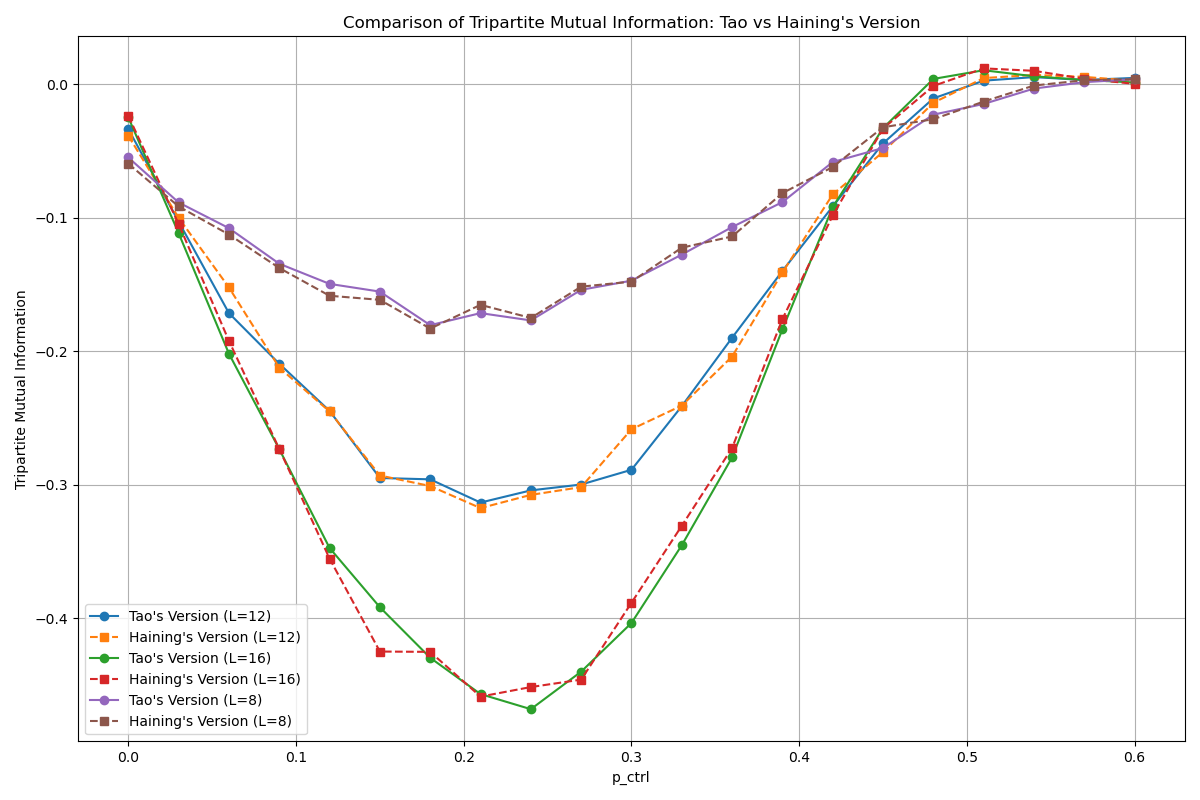
\includegraphics[width=0.8\linewidth]{tmi_comparison.png}
    \caption{Comparison of tripartite mutual information calculation between Haining's and developed codebase for the global adder with fixed point $\{1/3, 2/3\}$ at projective measurement rate of 0.3.}
    \label{fig:tmi_comparison}
\end{figure}

\subsection{Performance Analysis and Computational Requirements}

The next objective involves recreating the line of critical points in the phase diagram separating the area law phase and the compact area law phase using tripartite mutual information as the metric. This calculation requires substantial computational resources that would be impractical for local laptop execution.

Table \ref{tab:performance_comparison} presents a comprehensive performance comparison between the developed codebase and Haining's implementation, including projected total runtime estimates.

\begin{table}[h]
\centering
\begin{tabular}{|c|c|c|c|c|c|}
\hline
$L$ & Steps & $T_\text{Developed}$ (s) & $T_\text{Haining}$ (s) & $T_\text{Developed}^{\text{total}}$ (h) & $T_\text{Haining}^{\text{total}}$ (h) \\
\hline
6 & 72 & 0.005815 & 0.006403 & 0.07 & 0.07 \\
\hline
8 & 128 & 0.010986 & 0.012339 & 0.13 & 0.14 \\
\hline
10 & 200 & 0.021206 & 0.024297 & 0.25 & 0.28 \\
\hline
12 & 288 & 0.054367 & 0.061841 & 0.63 & 0.72 \\
\hline
14 & 392 & 0.306082 & 0.346021 & 3.57 & 4.04 \\
\hline
16 & 512 & 1.316186 & 1.551793 & 15.36 & 18.10 \\
\hline
\end{tabular}
\caption{Performance comparison between developed and Haining's codebase for AFM Global with projective measurement, with estimated total runtime for 2000 iterations and 21 $p_\text{ctrl}$ control rates ranging from 0 to 1. The number of time steps in the evolution is $2L^2$.}
\label{tab:performance_comparison}
\end{table}

The analysis indicates that 16-qubit calculations require nearly a full day on local hardware, making L=20,24 computations impractical without high-performance computing resources.

\subsection{Finite Size Scaling Analysis}

Finite Size Scaling (FSS) analysis was performed to extract critical points $p_c$ and critical dynamical exponents $\nu$ using Haining's codebase for system sizes $\{12, 16, 20\}$ with an ensemble size of 2000 samples. Analysis focused on two critical points: $p_\text{ctrl}=0.0$ and $p_\text{ctrl}=0.4$ with projective measurement, as shown in the phase diagram (Figure \ref{fig:phase_diagram}).

\begin{figure}[H]
    \centering
    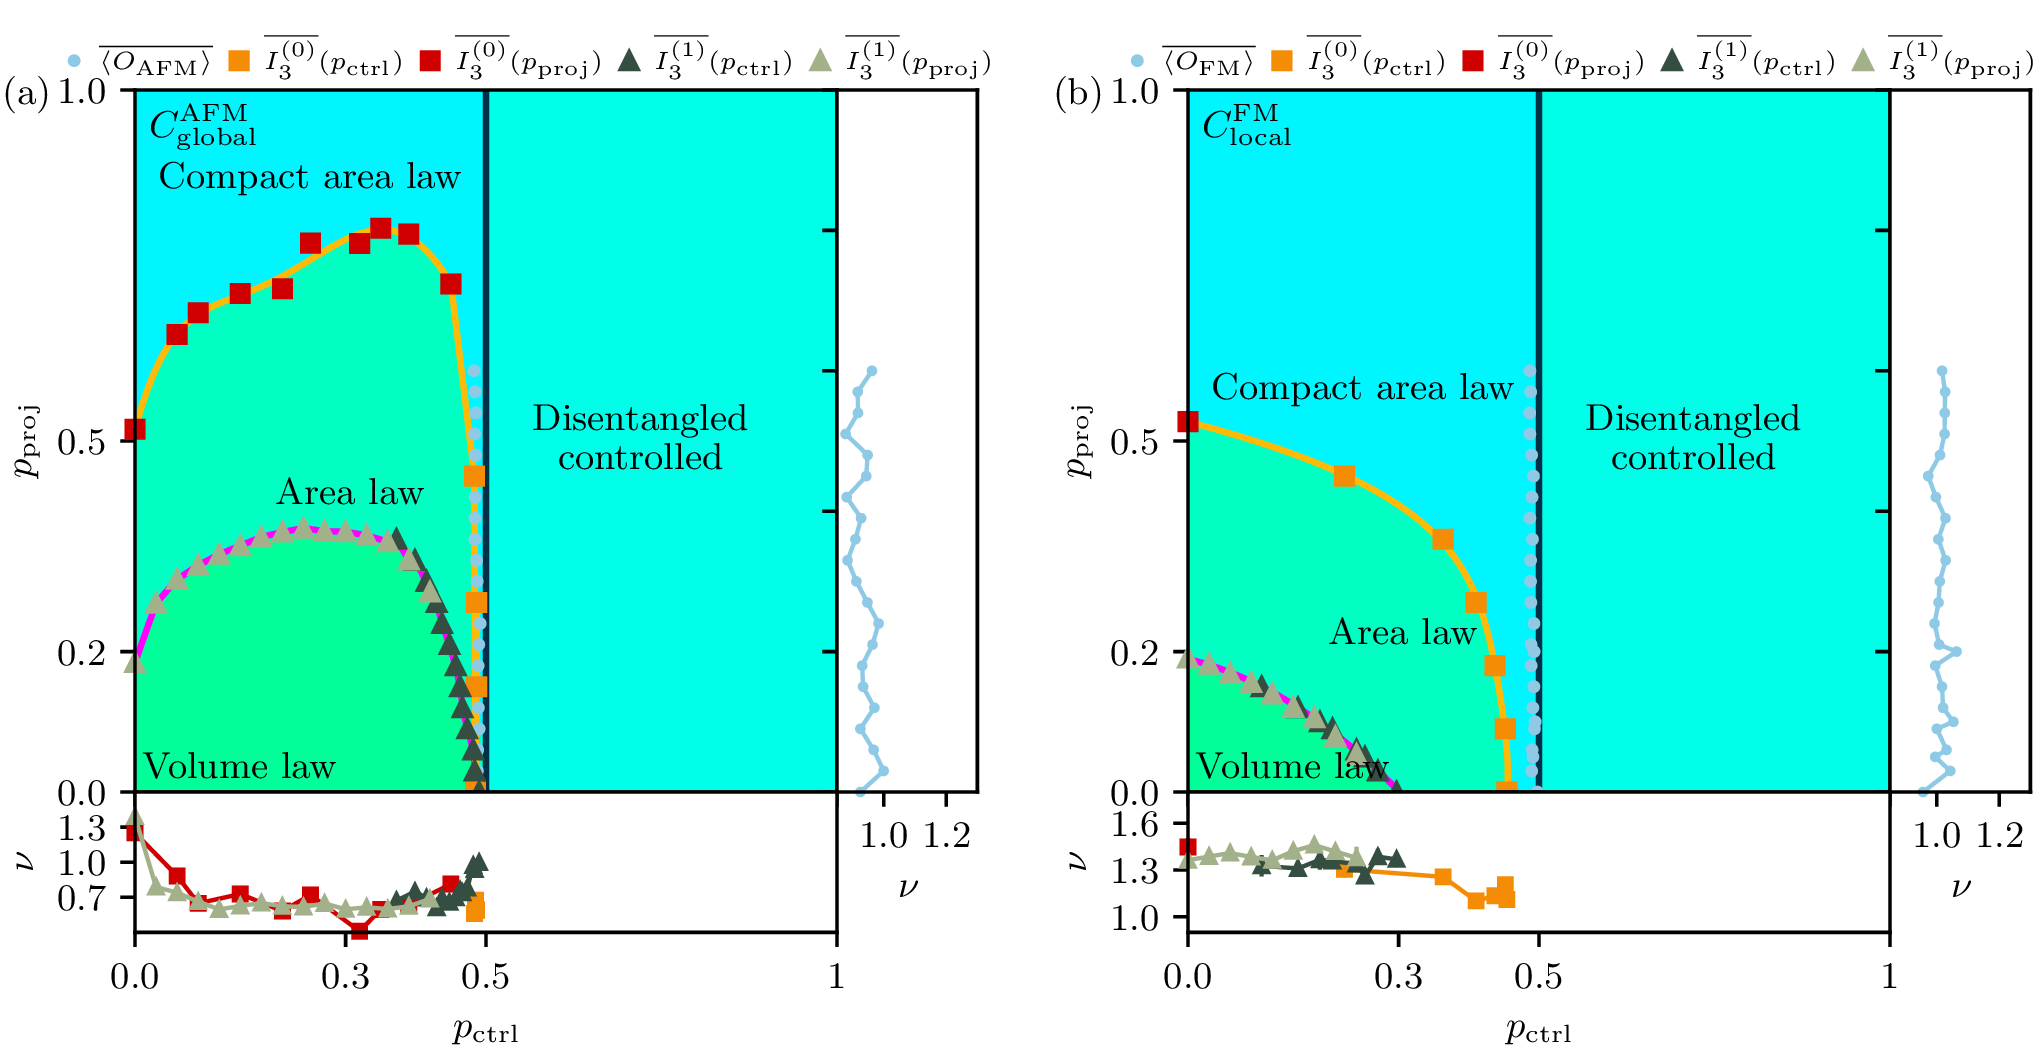
\includegraphics[width=0.8\linewidth]{pd.png}
    \caption{Phase diagram of the control transition for the global adder with projective measurement.}
    \label{fig:phase_diagram}
\end{figure}

\subsubsection{Critical Point Analysis: $p_\text{ctrl}=0.0$}

For the first critical point examined ($p_\text{ctrl}=0.0$), analytical results are available: $p_c=0.5$ and $\nu=4/3$. Numerical results from the developed codebase yielded $p_c=0.491$ and $\nu=1.369$. Figure \ref{fig:fss_analysis_comparison} presents the FSS analysis comparison between implementations.

\begin{figure}[H]
    \centering
    \begin{subfigure}[t]{0.8\linewidth}
        \centering
        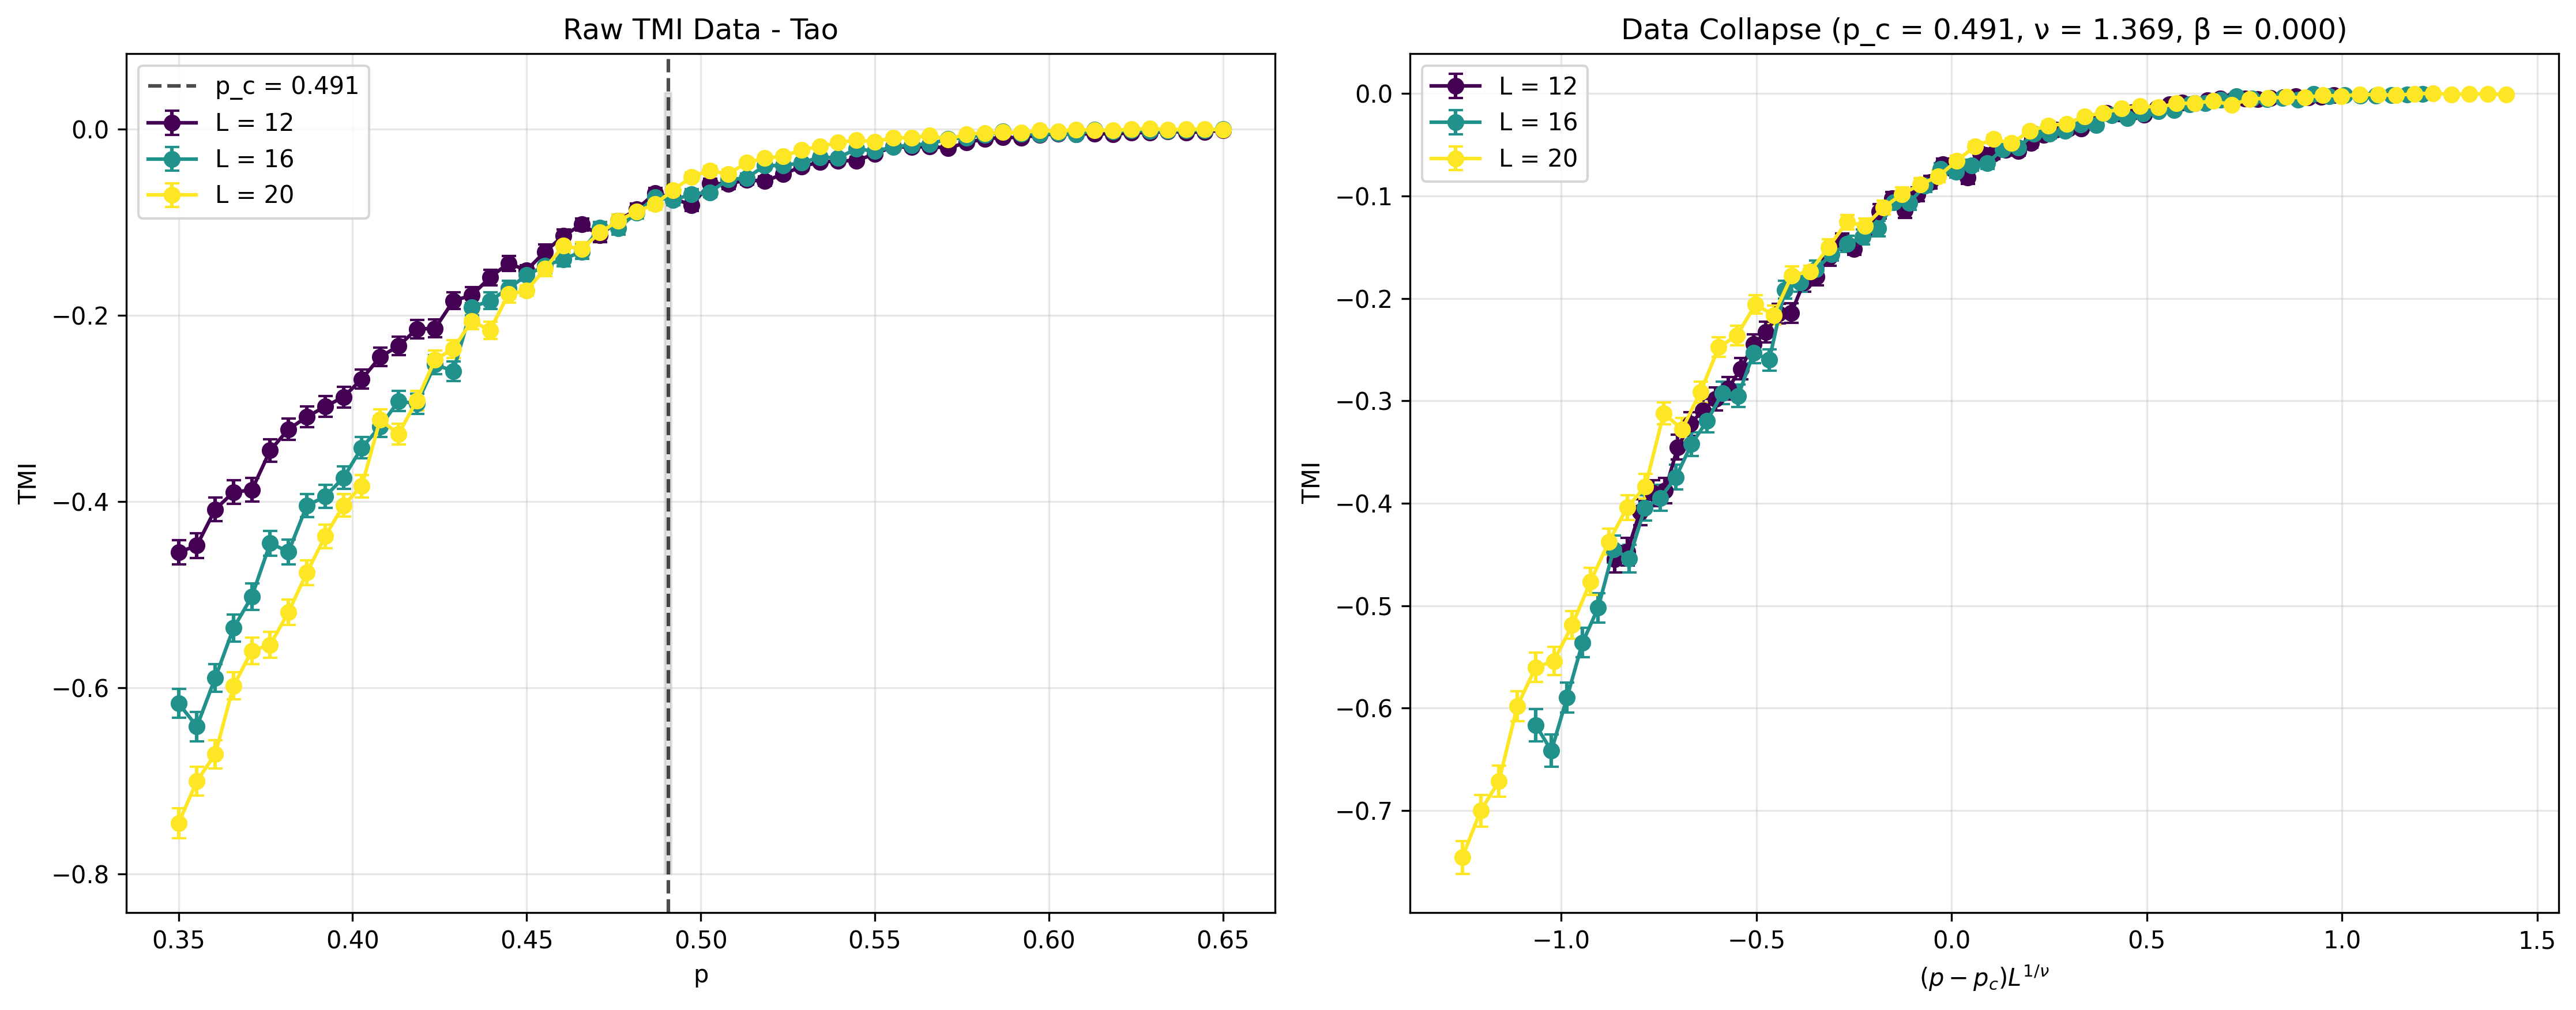
\includegraphics[width=\linewidth]{data_collapse_tao_pctrl0.000_threshold1.0e-15.png}
        \caption{Critical scaling of tripartite mutual information with developed codebase.}
        \label{fig:fss_analysis_developed}
    \end{subfigure}
    \vfill
    \begin{subfigure}[b]{0.8\linewidth}
        \centering
        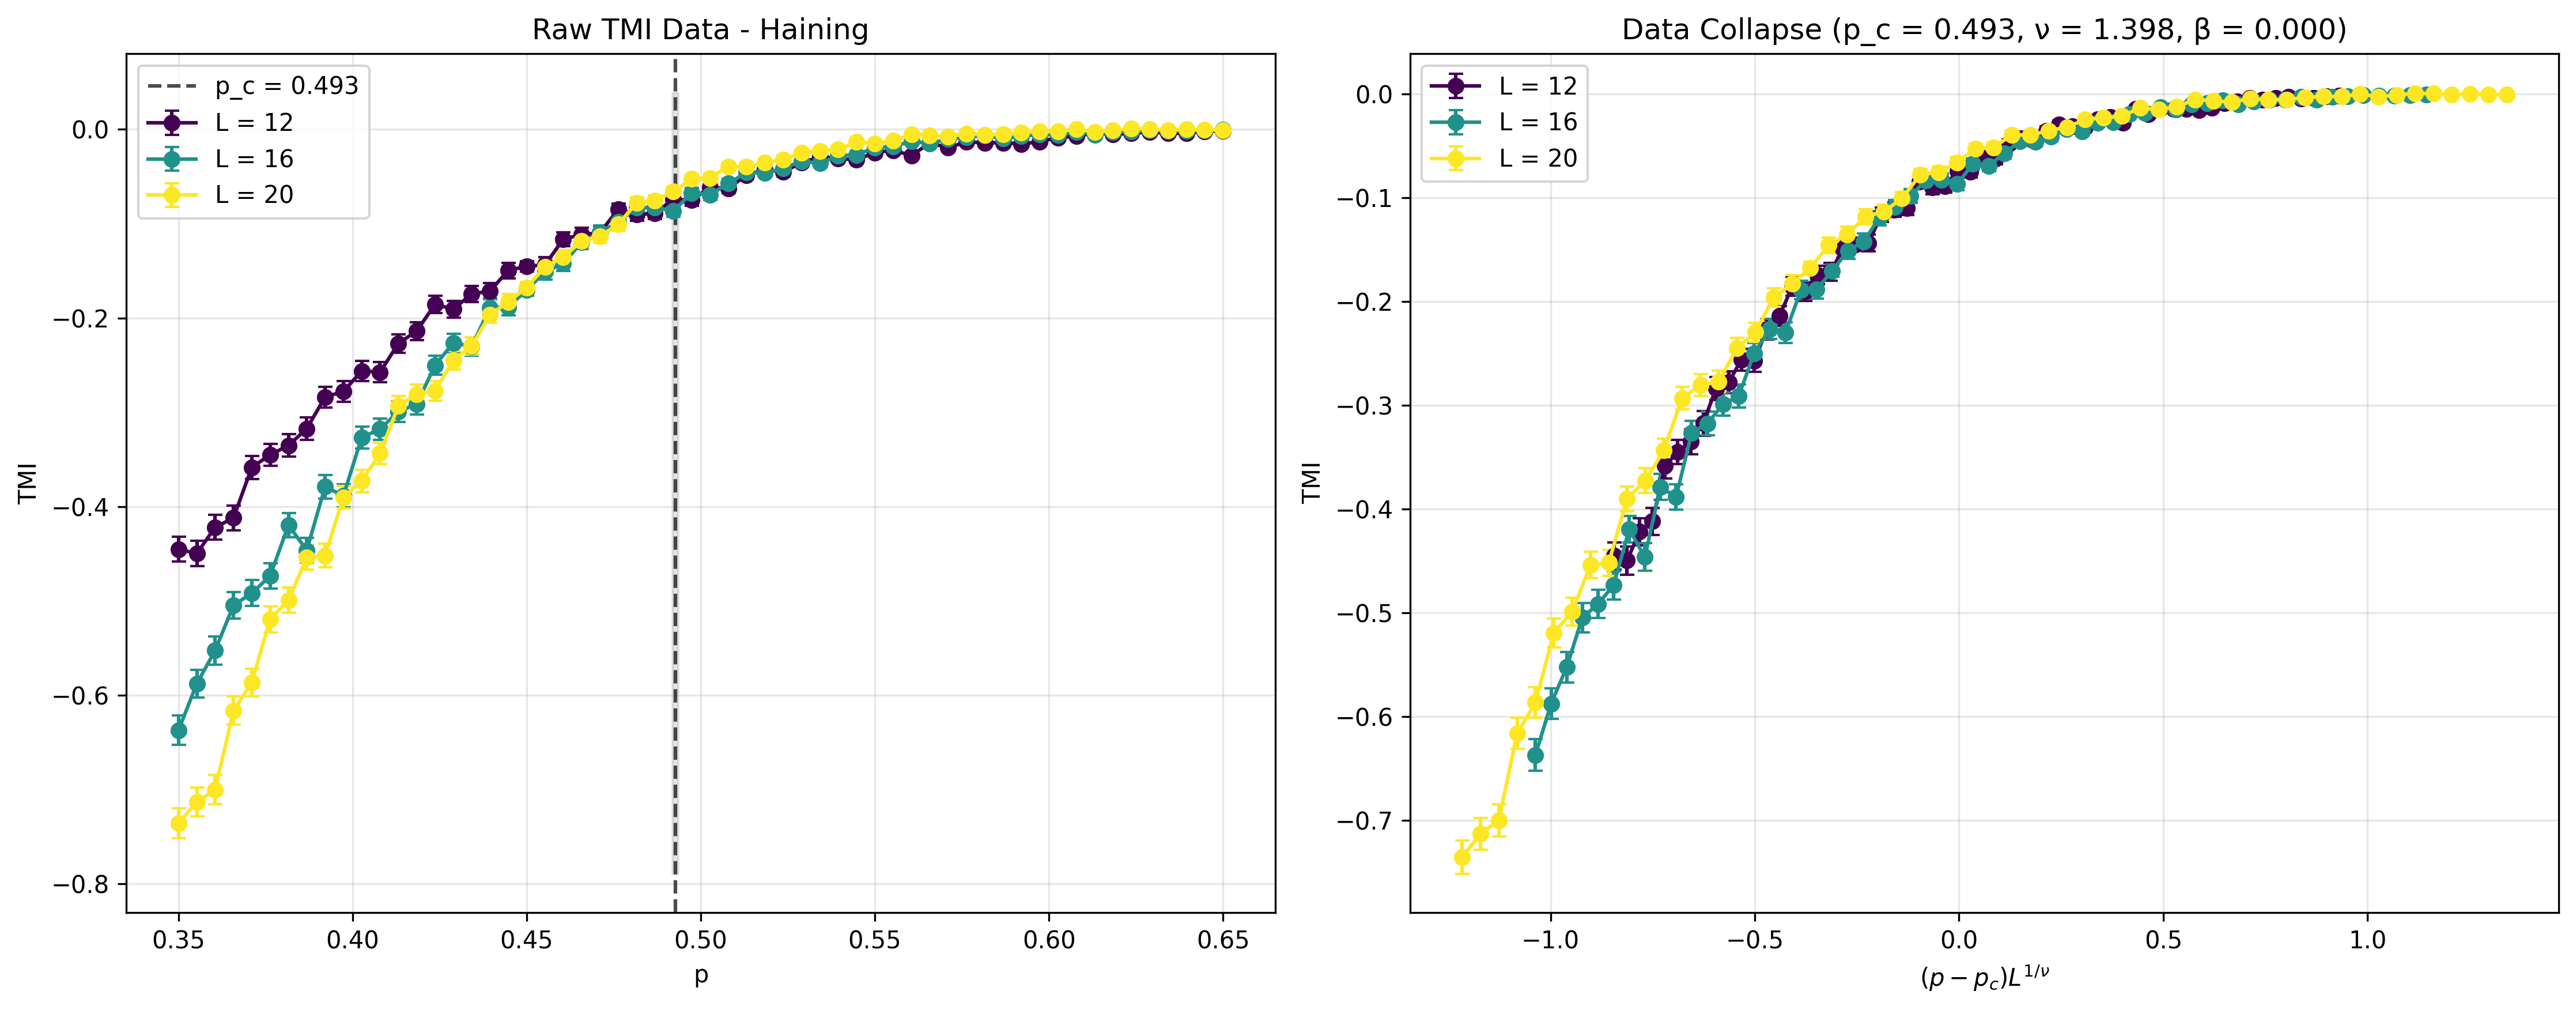
\includegraphics[width=\linewidth]{data_collapse_haining_pctrl0.000_threshold1.0e-15.png}
        \caption{Critical scaling of tripartite mutual information with Haining's codebase.}
        \label{fig:fss_analysis_haining}
    \end{subfigure}
    \caption{Critical scaling of tripartite mutual information with developed codebase (top) and Haining's codebase (bottom) with $p_\text{ctrl}=0.0$ and threshold value $1.0\times10^{-15}$.}
    \label{fig:fss_analysis_comparison}
\end{figure}

\subsubsection{Numerical Stability Investigation}

To investigate the numerical stability of the FSS analysis, contour plots of the loss function $\chi^2$ as a function of $p_c$ and $\nu$ were generated (Figure \ref{fig:chi2_contour}).

\begin{figure}[H]
    \centering
    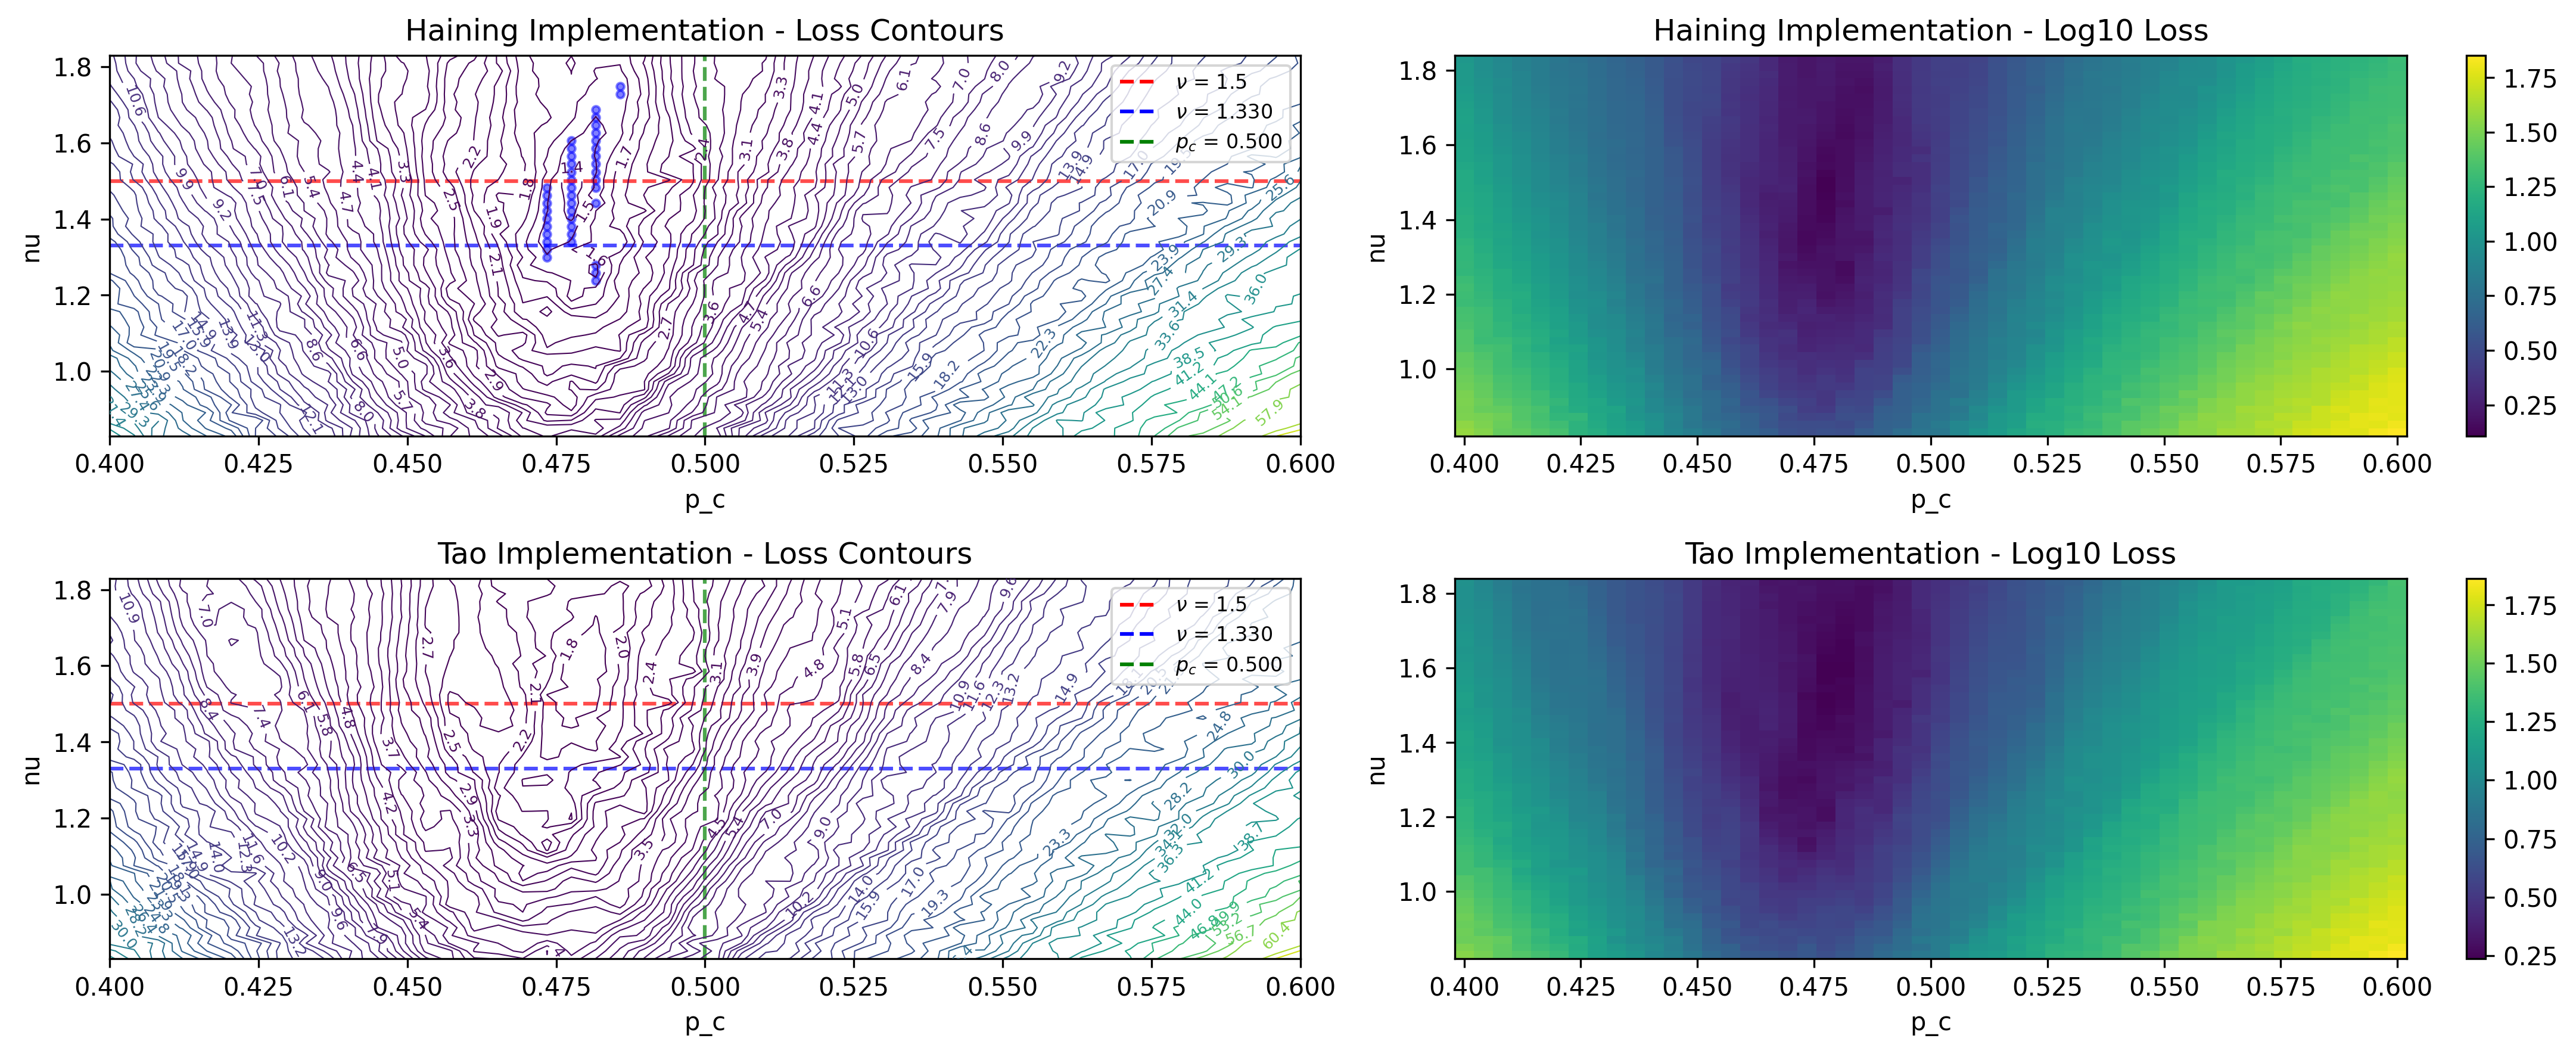
\includegraphics[width=0.8\linewidth]{loss_manifold_comparison_pctrl0.000_threshold1.0e-15.png}
    \caption{Contour of the loss function $\chi^2$ as a function of $p_c$ and $\nu$.}
    \label{fig:chi2_contour}
\end{figure}

The contour analysis reveals significantly larger error bars in the $\nu$ direction compared to the $p_c$ direction. Figure \ref{fig:p_nu_threshold_combined} shows the best fit results for $p_c$ and $\nu$ as functions of decreasing Rényi entropy threshold.

\begin{figure}[H]
    \centering
    \begin{subfigure}[b]{0.48\linewidth}
        \centering
        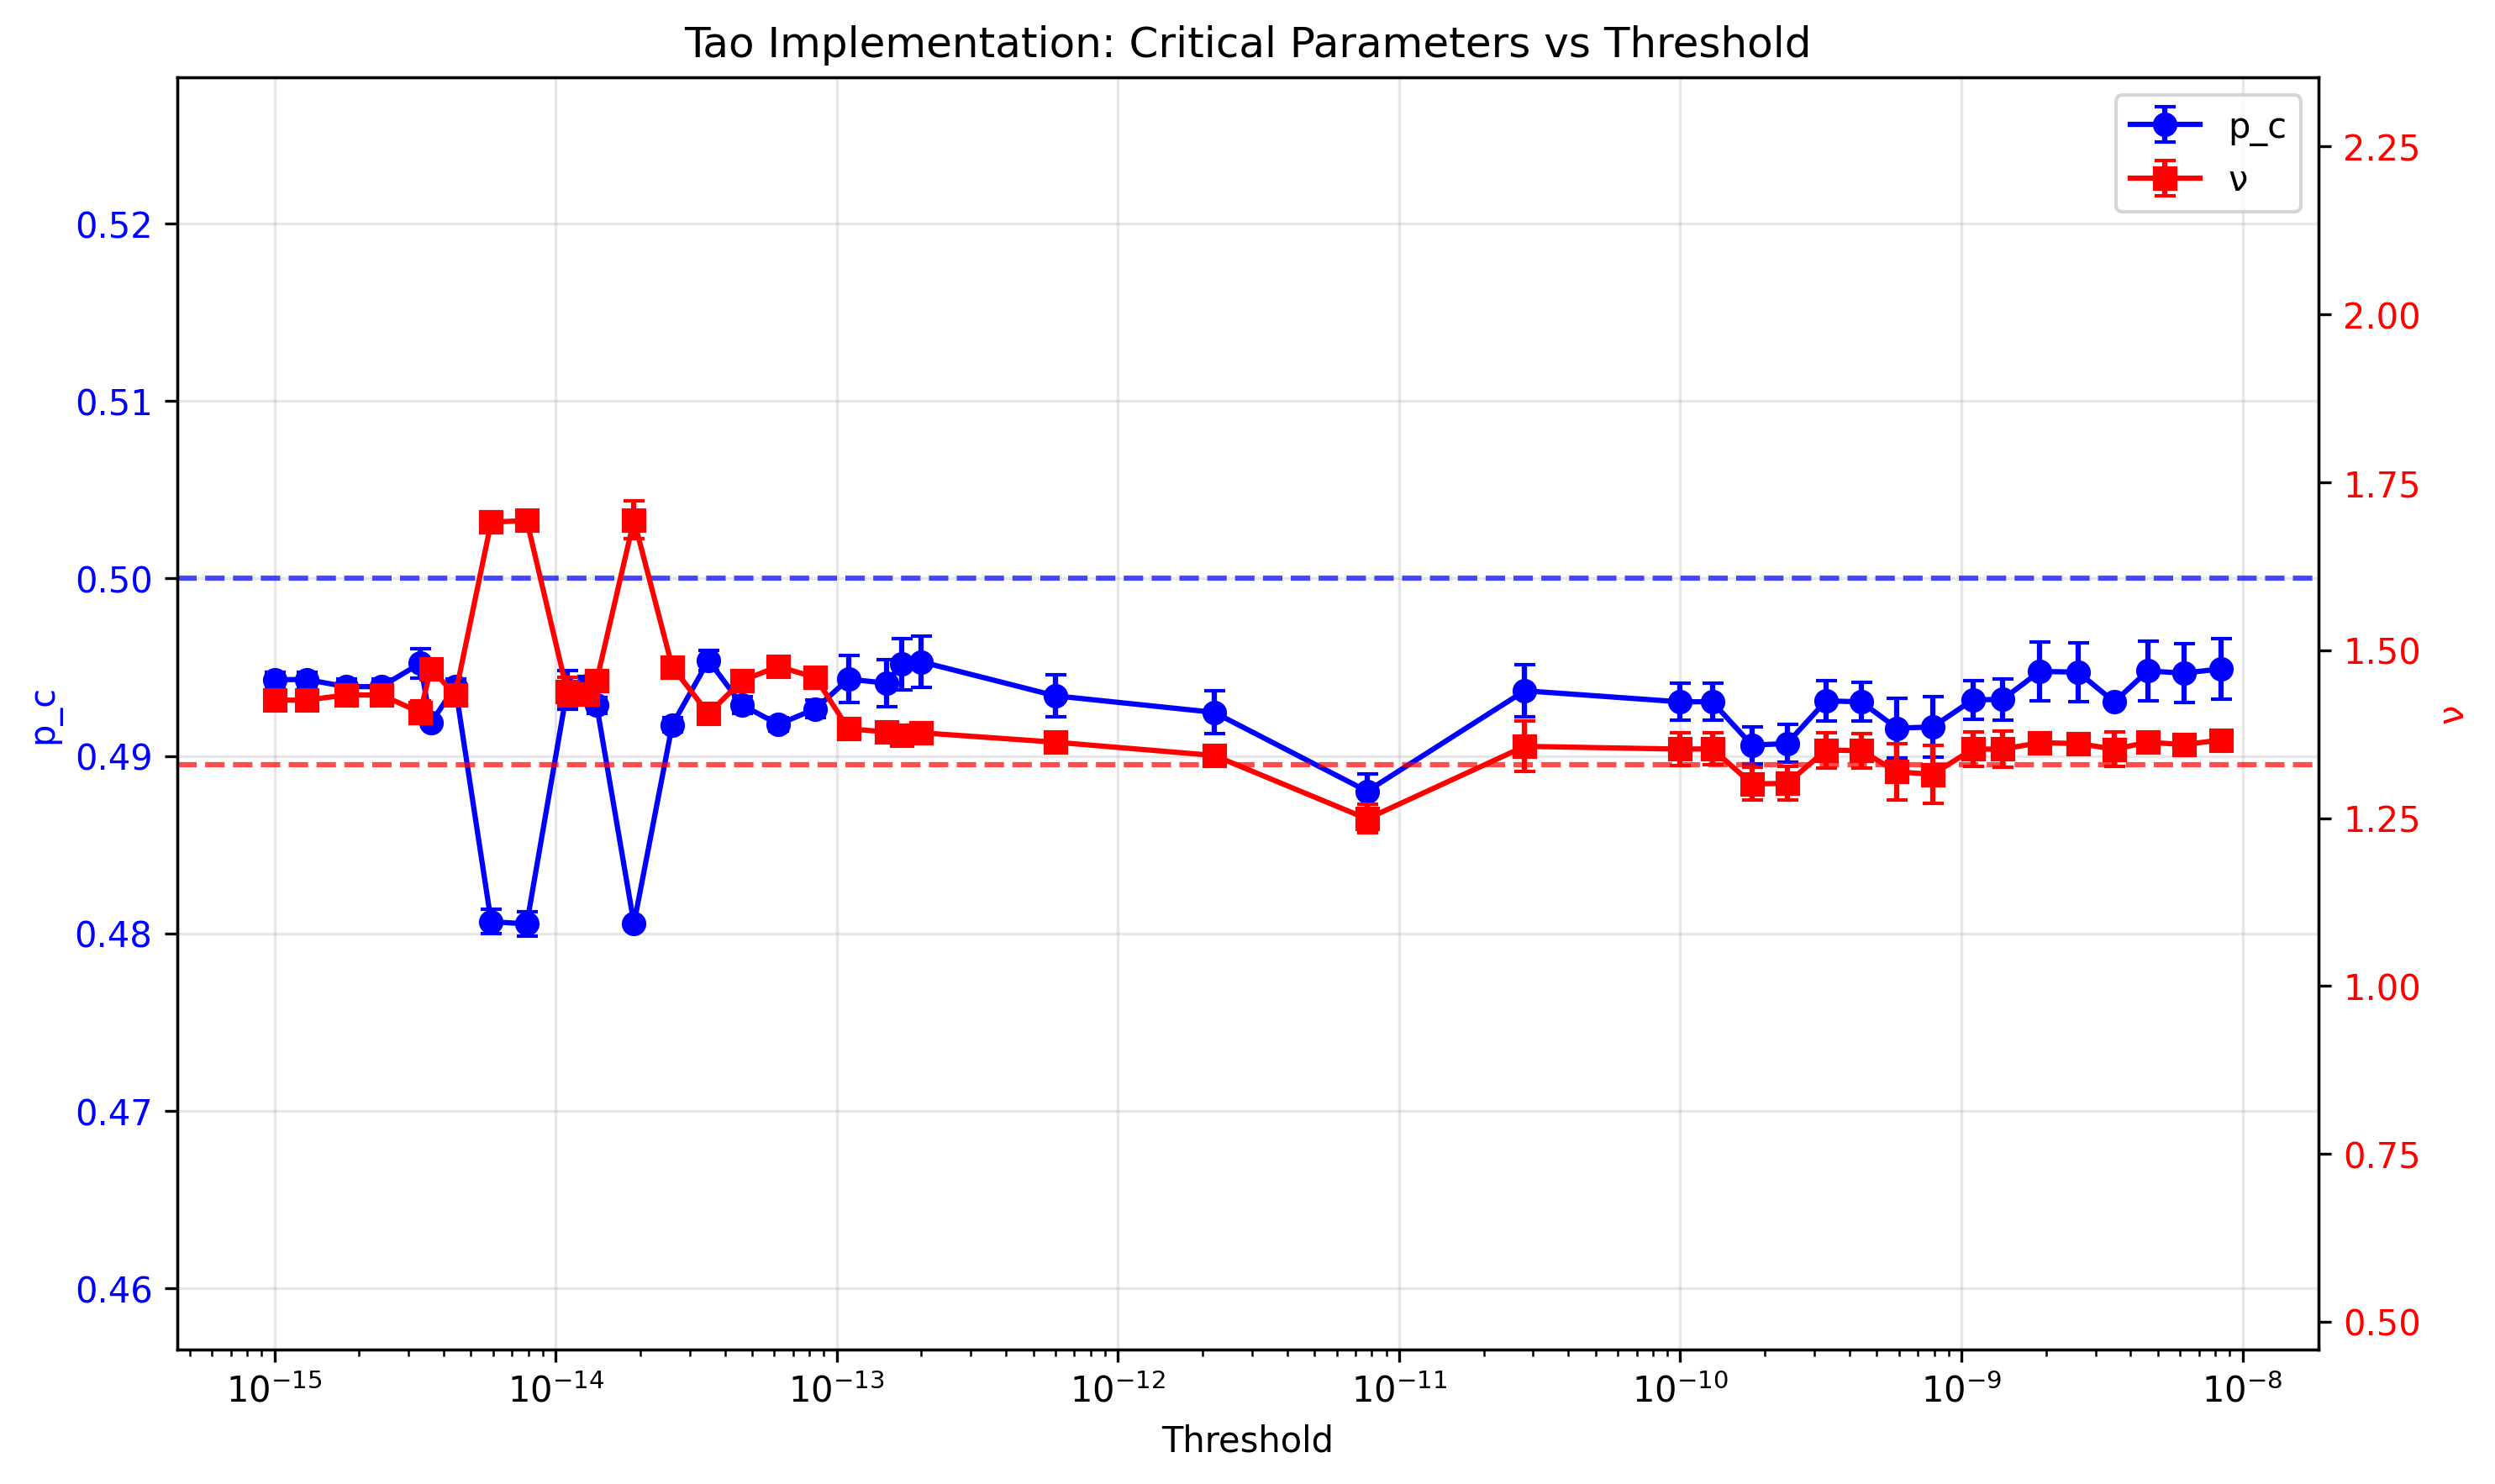
\includegraphics[width=\linewidth]{threshold_dependence_tao.png}
        \caption{Results from developed codebase}
        \label{fig:p_nu_threshold_developed}
    \end{subfigure}
    \hfill
    \begin{subfigure}[b]{0.48\linewidth}
        \centering
        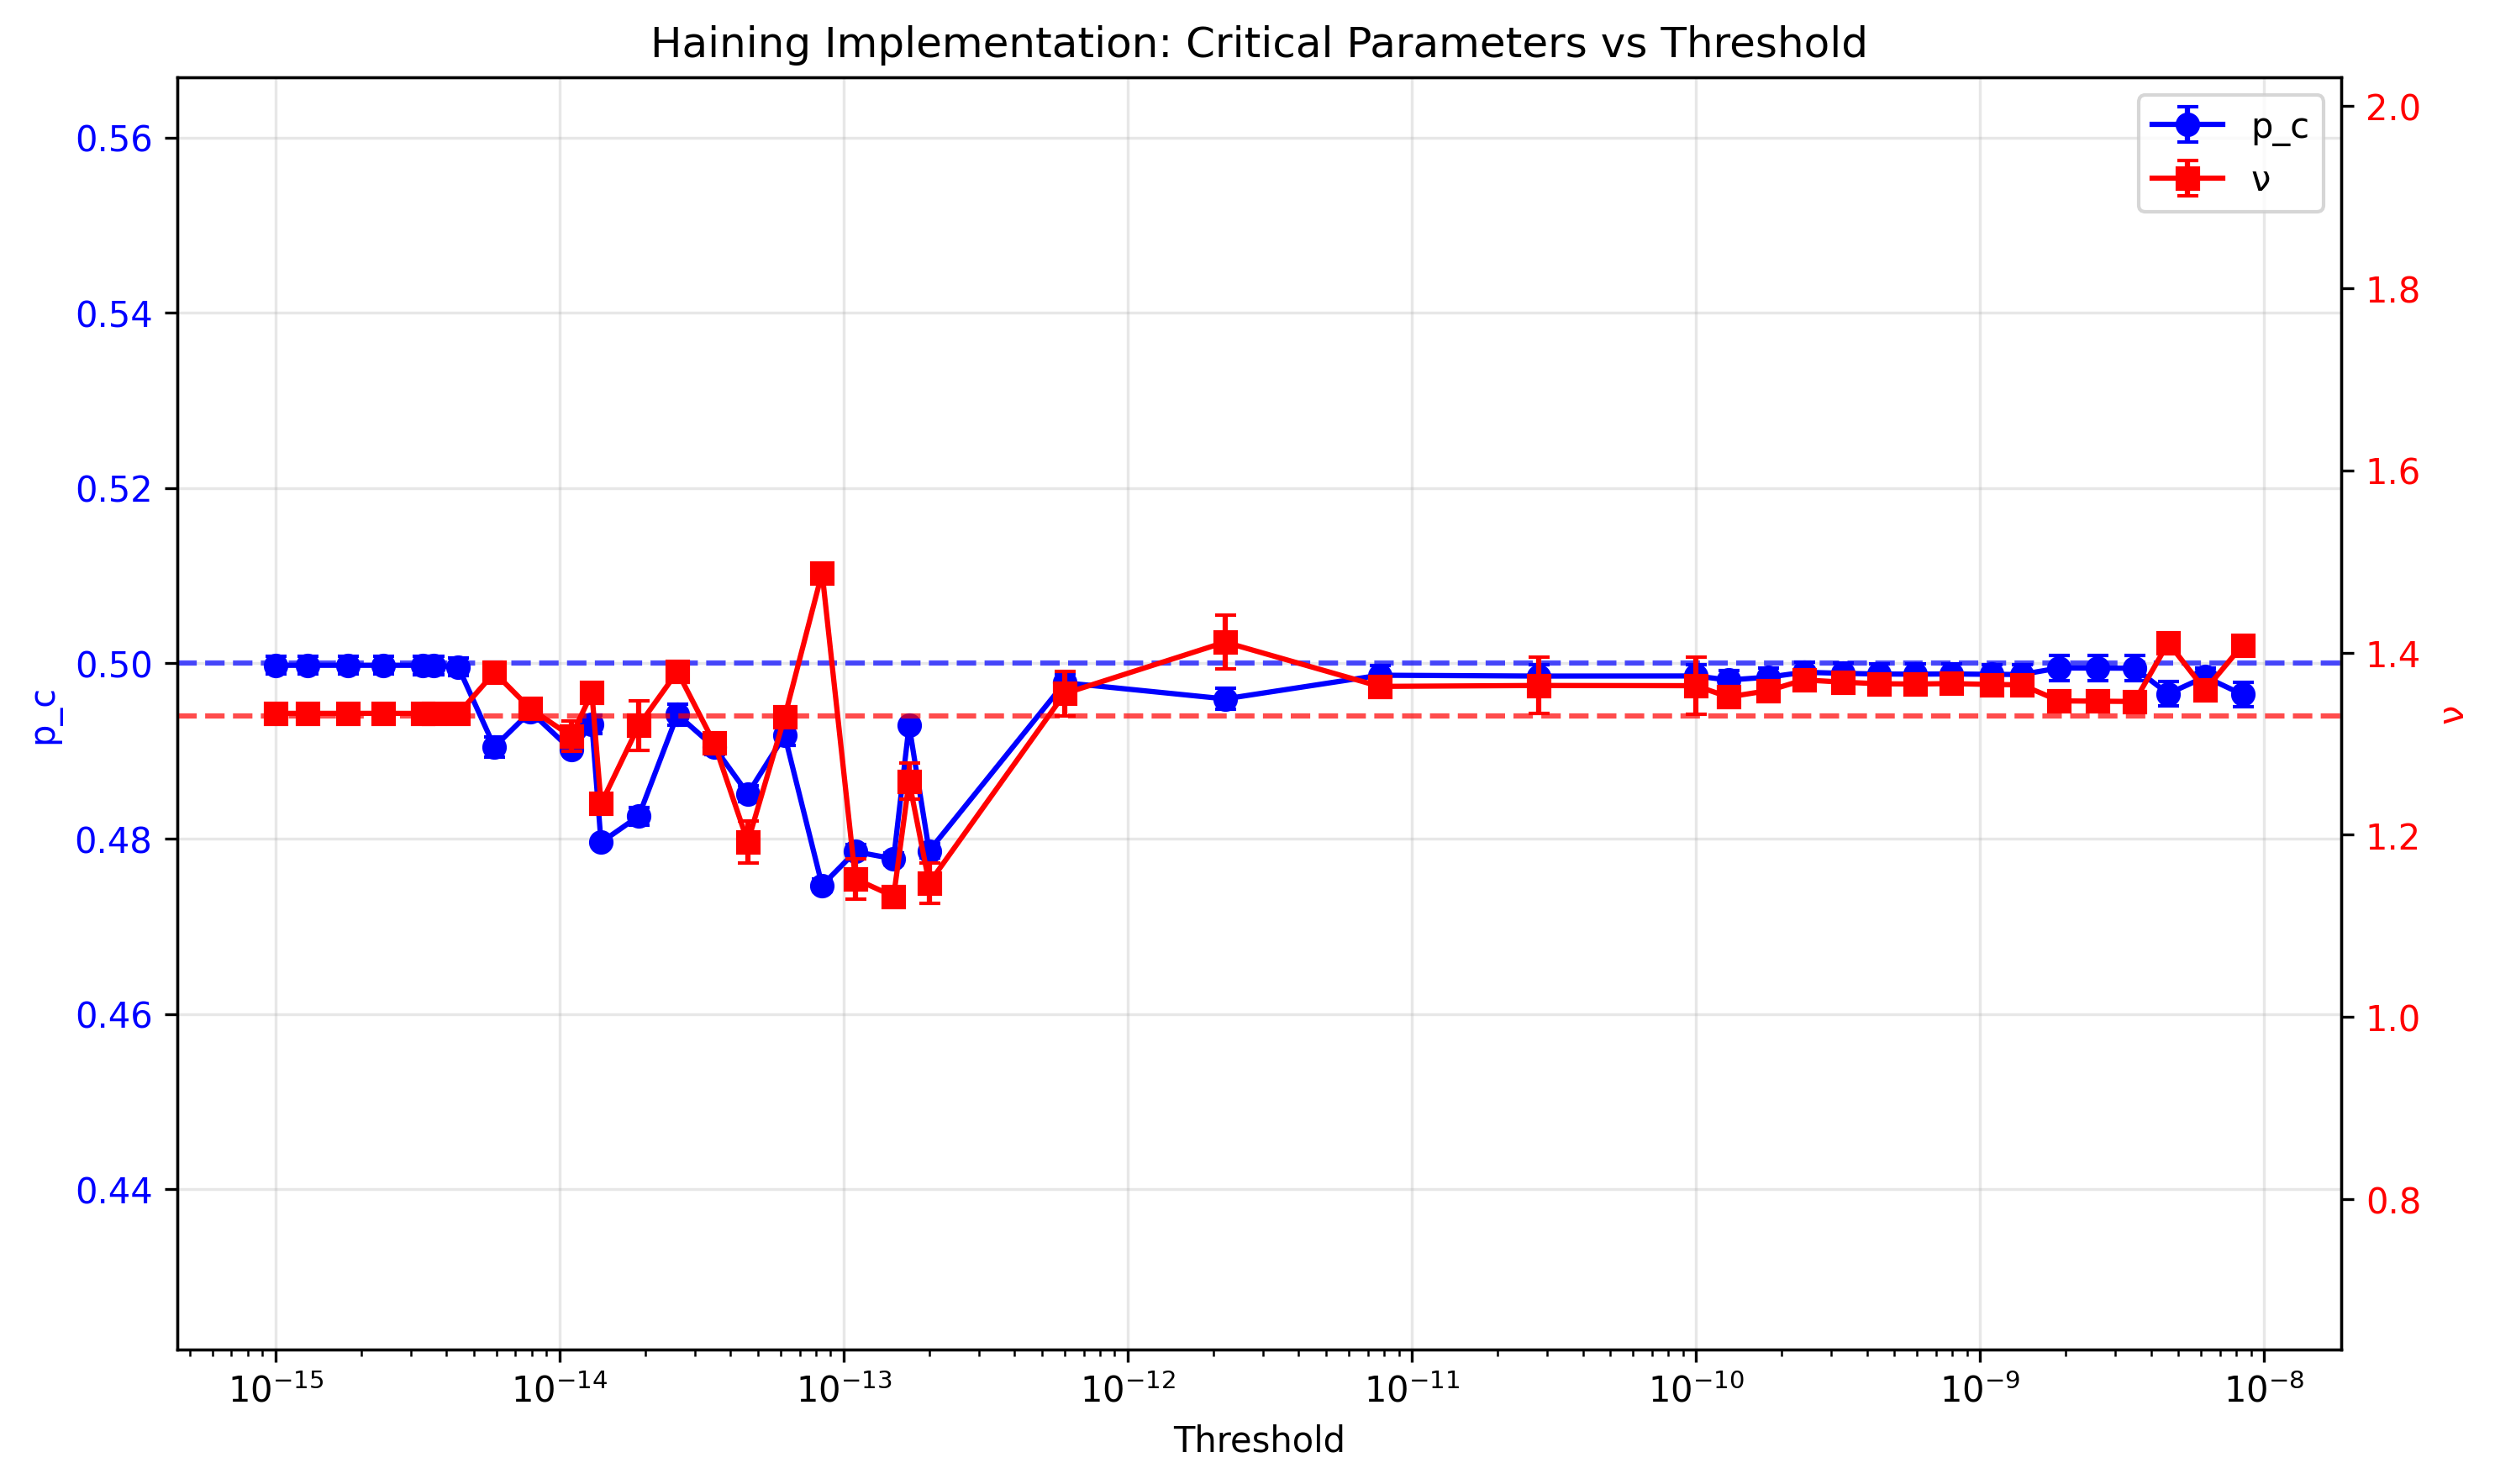
\includegraphics[width=\linewidth]{threshold_dependence_haining.png}
        \caption{Results from Haining's codebase}
        \label{fig:p_nu_threshold_haining}
    \end{subfigure}
    \caption{Best fit results for $p_c$ and $\nu$ as a function of decreasing threshold of the Rényi entropy.}
    \label{fig:p_nu_threshold_combined}
\end{figure}

The developed codebase demonstrates less numerical stability compared to Haining's implementation. Analysis of low-lying loss points on the loss manifold (Figure \ref{fig:loss_manifolds_combined}) reveals wider standard deviation in the $\nu$ direction for the developed implementation.

\begin{figure}[H]
    \centering
    \begin{subfigure}[t]{0.8\linewidth}
        \centering
        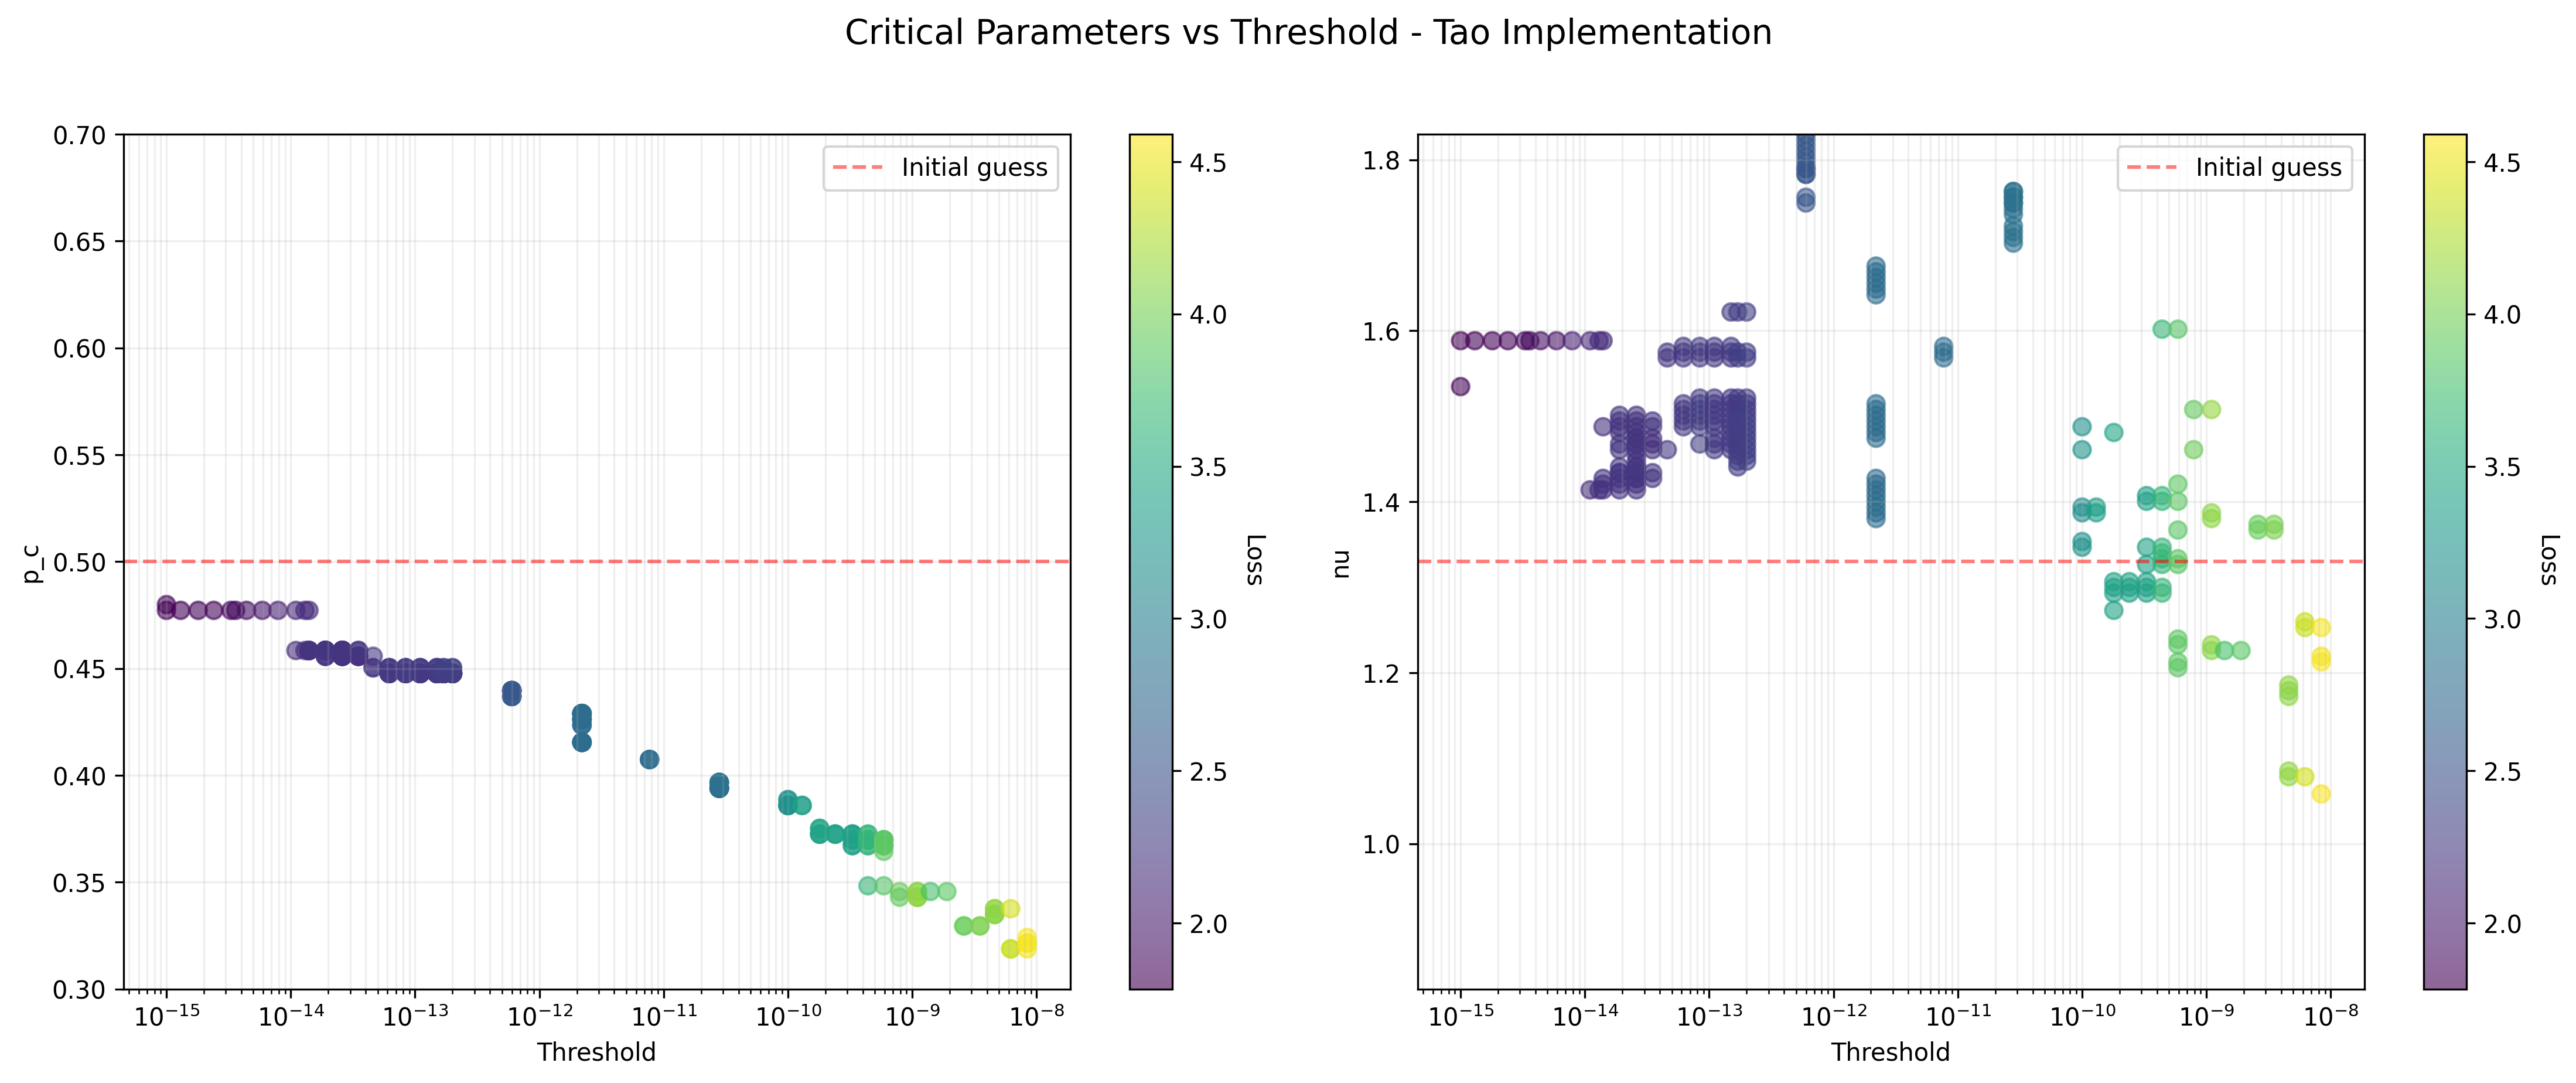
\includegraphics[width=\linewidth]{threshold_dependence_pctrl0.000_tao.png}
        \caption{Low loss points from FSS analysis with developed codebase.}
        \label{fig:loss_manifold_developed}
    \end{subfigure}
    \vfill
    \begin{subfigure}[b]{0.8\linewidth}
        \centering
        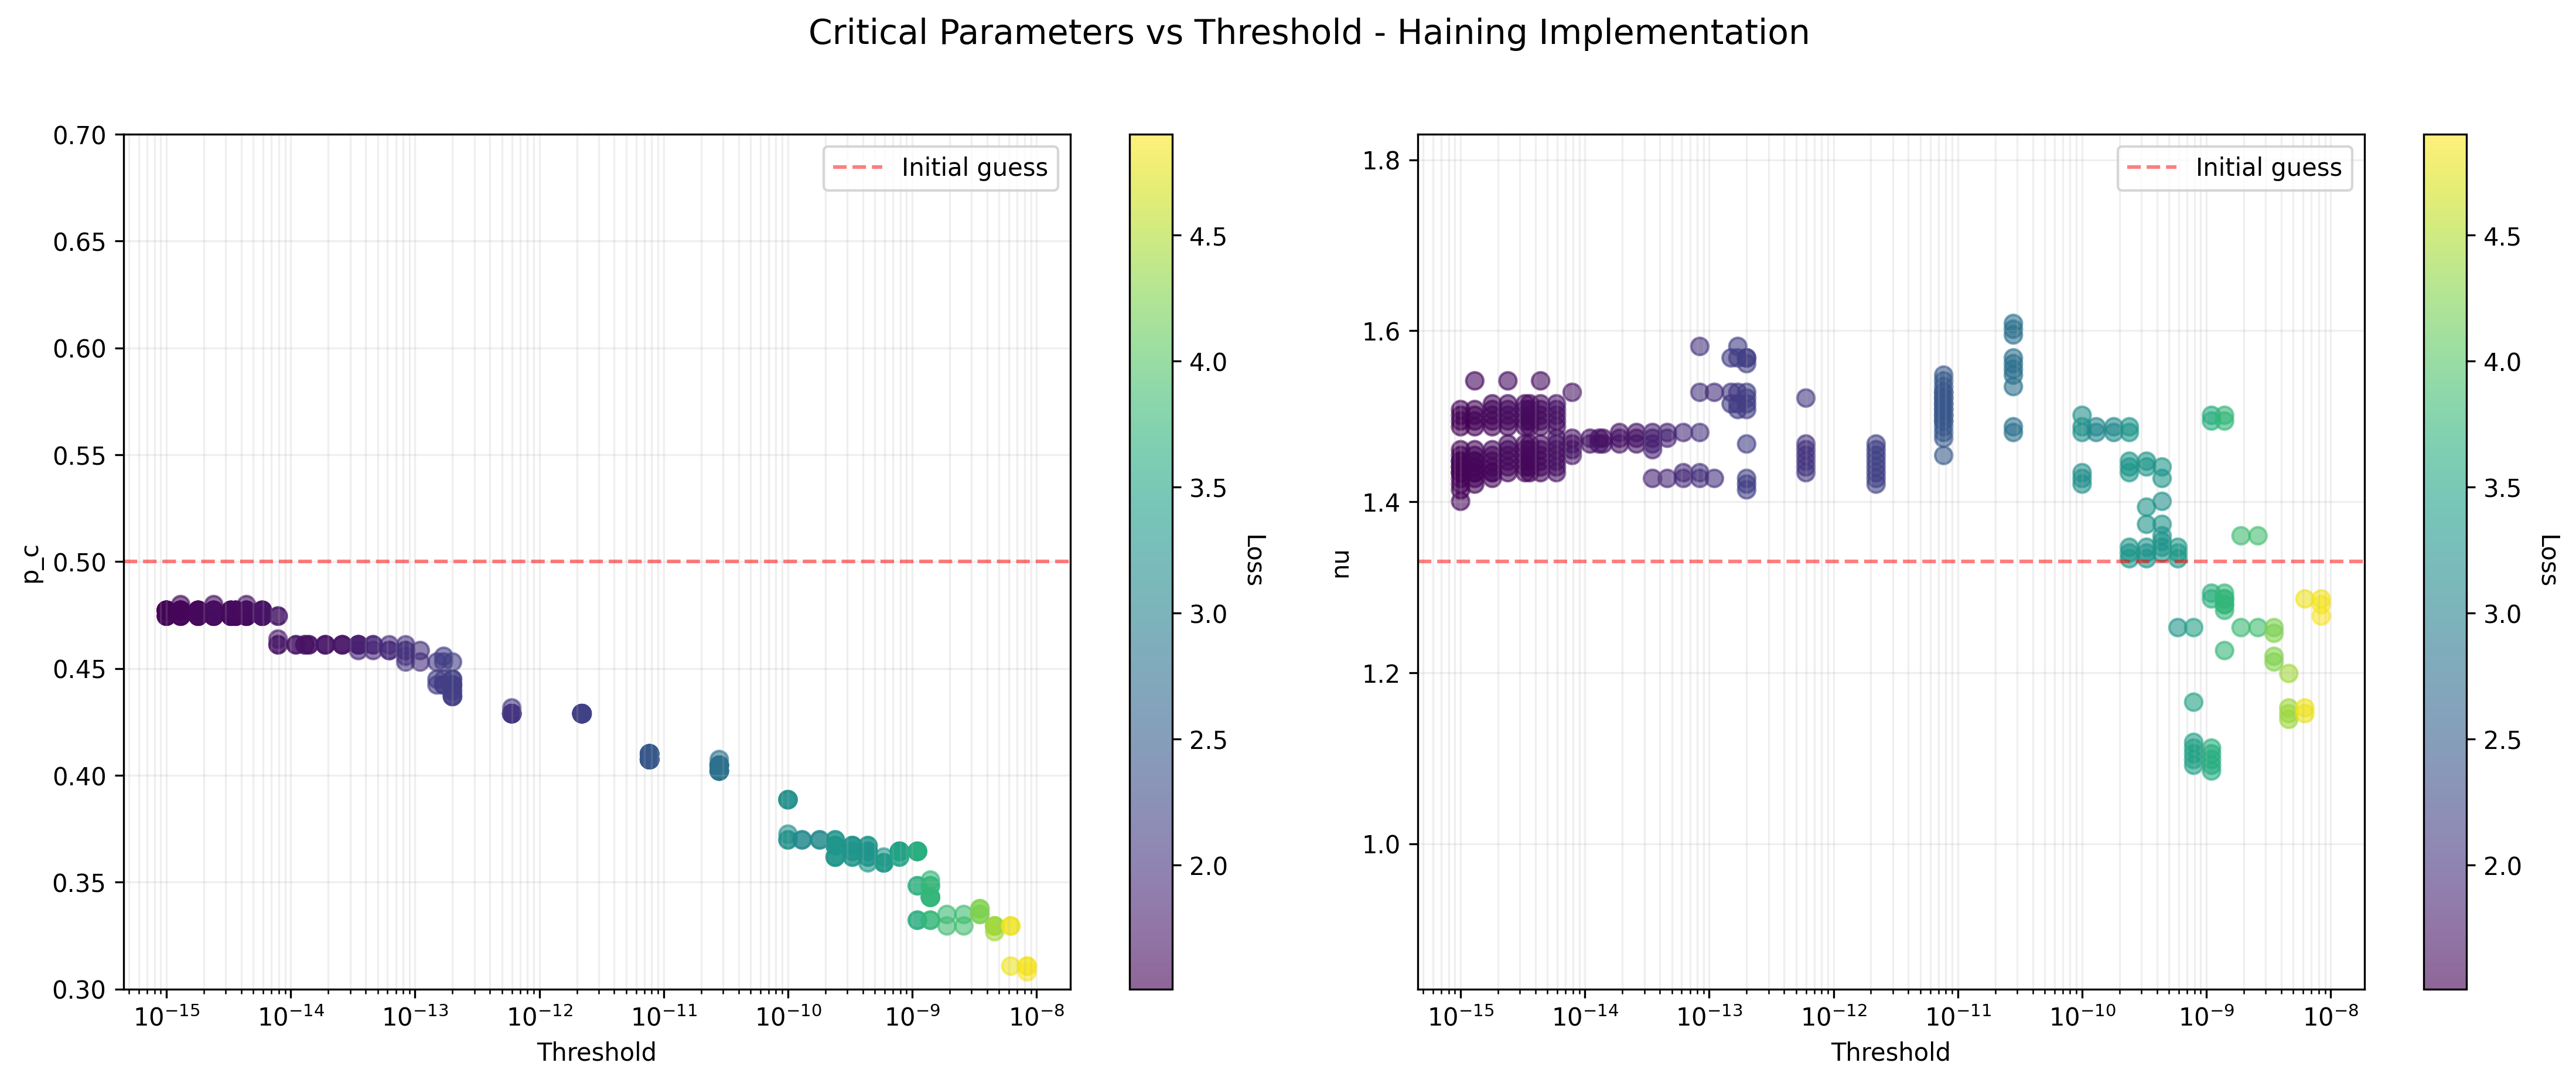
\includegraphics[width=\linewidth]{threshold_dependence_pctrl0.000_haining.png}
        \caption{Low loss points from FSS analysis with Haining's codebase.}
        \label{fig:loss_manifold_haining}
    \end{subfigure}
    \caption{Low loss points from FSS analysis with different codebases.}
    \label{fig:loss_manifolds_combined}
\end{figure}

The loss manifold from the developed codebase appears more discontinuous with a wider basin of attraction, suggesting increased likelihood of gradient descent convergence to local minima.

\subsubsection{Singular Value Computation Analysis}

Investigation into the numerical discrepancies identified differences in singular value computation methods. Haining's codebase computes singular values as follows:

\begin{lstlisting}[language=Python]
vec_tensor_T = vec_tensor.transpose(np.hstack([subregion, not_subregion]))
S = np.linalg.svd(vec_tensor_T.reshape((2**len(subregion), 2**len(not_subregion))), compute_uv=False)
\end{lstlisting}

The developed codebase implements an optimization by comparing subregion sizes and using the smaller dimension:

\begin{lstlisting}[language=Python]
vec_tensor = vec.reshape((2,) * L_T)
if len(subregion) < len(not_subregion):
    S = np.linalg.svd(vec_tensor.reshape((2**len(subregion), 2**len(not_subregion))), compute_uv=False)
else:
    S = np.linalg.svd(vec_tensor.reshape((2**len(not_subregion), 2**len(subregion))), compute_uv=False)
\end{lstlisting}

\subsubsection{Critical Point Analysis: $p_\text{ctrl}=0.4$}

Analysis of the second critical point ($p_\text{ctrl}=0.4$) where the published values are approximately $p_c=0.75$ and $\nu=0.7$ is presented in Figure \ref{fig:fss_analysis_combined_pctrl0.400}.

\begin{figure}[H]
    \centering
    \begin{subfigure}[t]{0.8\linewidth}
        \centering
        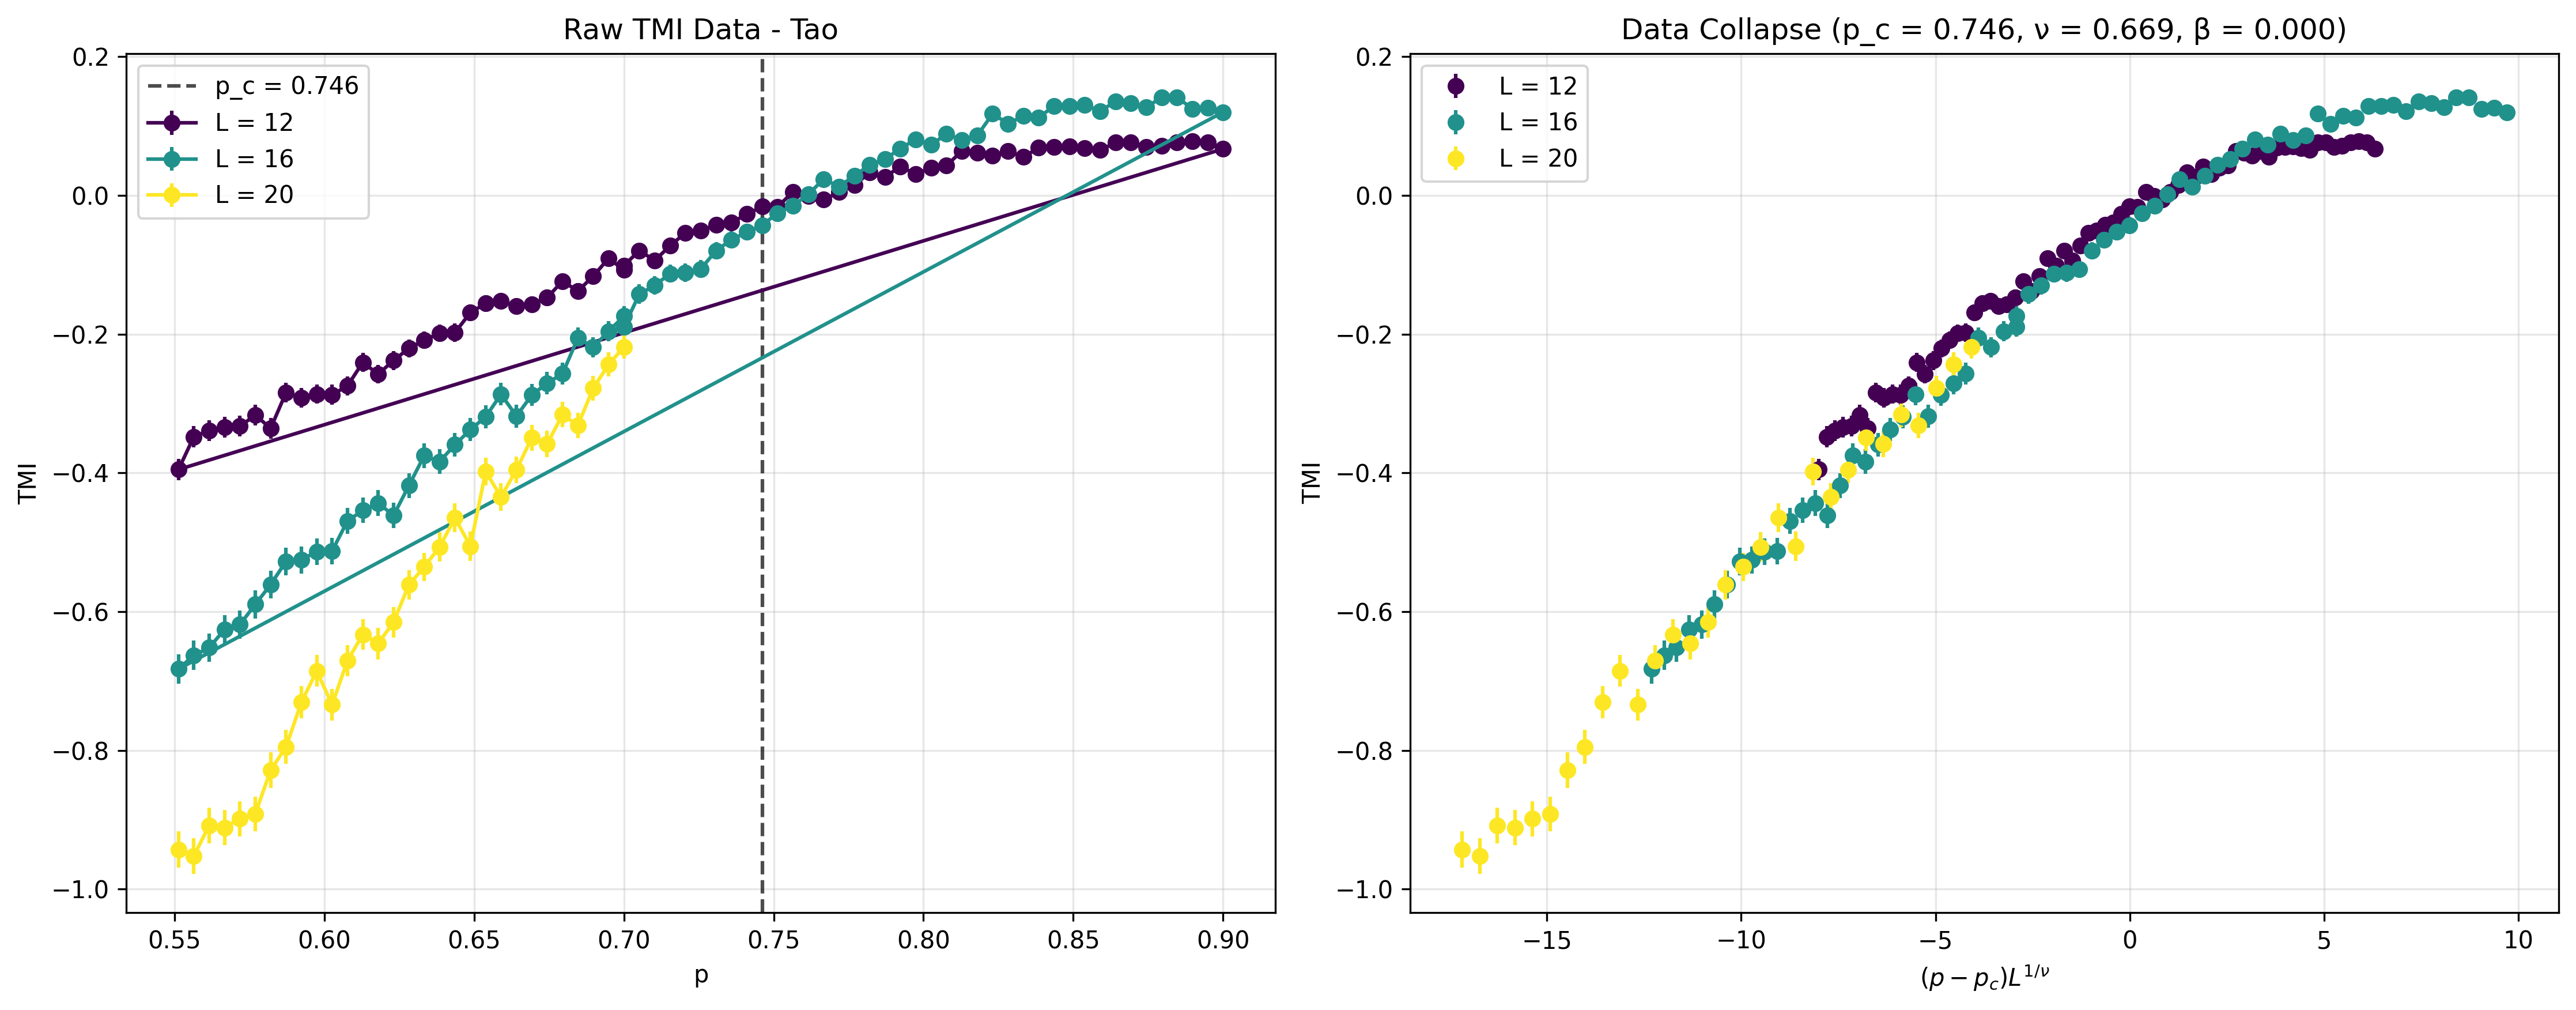
\includegraphics[width=\linewidth]{data_collapse_tao_pctrl0.400_threshold1.0e-15.png}
        \caption{FSS analysis with developed codebase.}
        \label{fig:fss_analysis_developed_pctrl0.400}
    \end{subfigure}
    \vfill
    \begin{subfigure}[b]{0.8\linewidth}
        \centering
        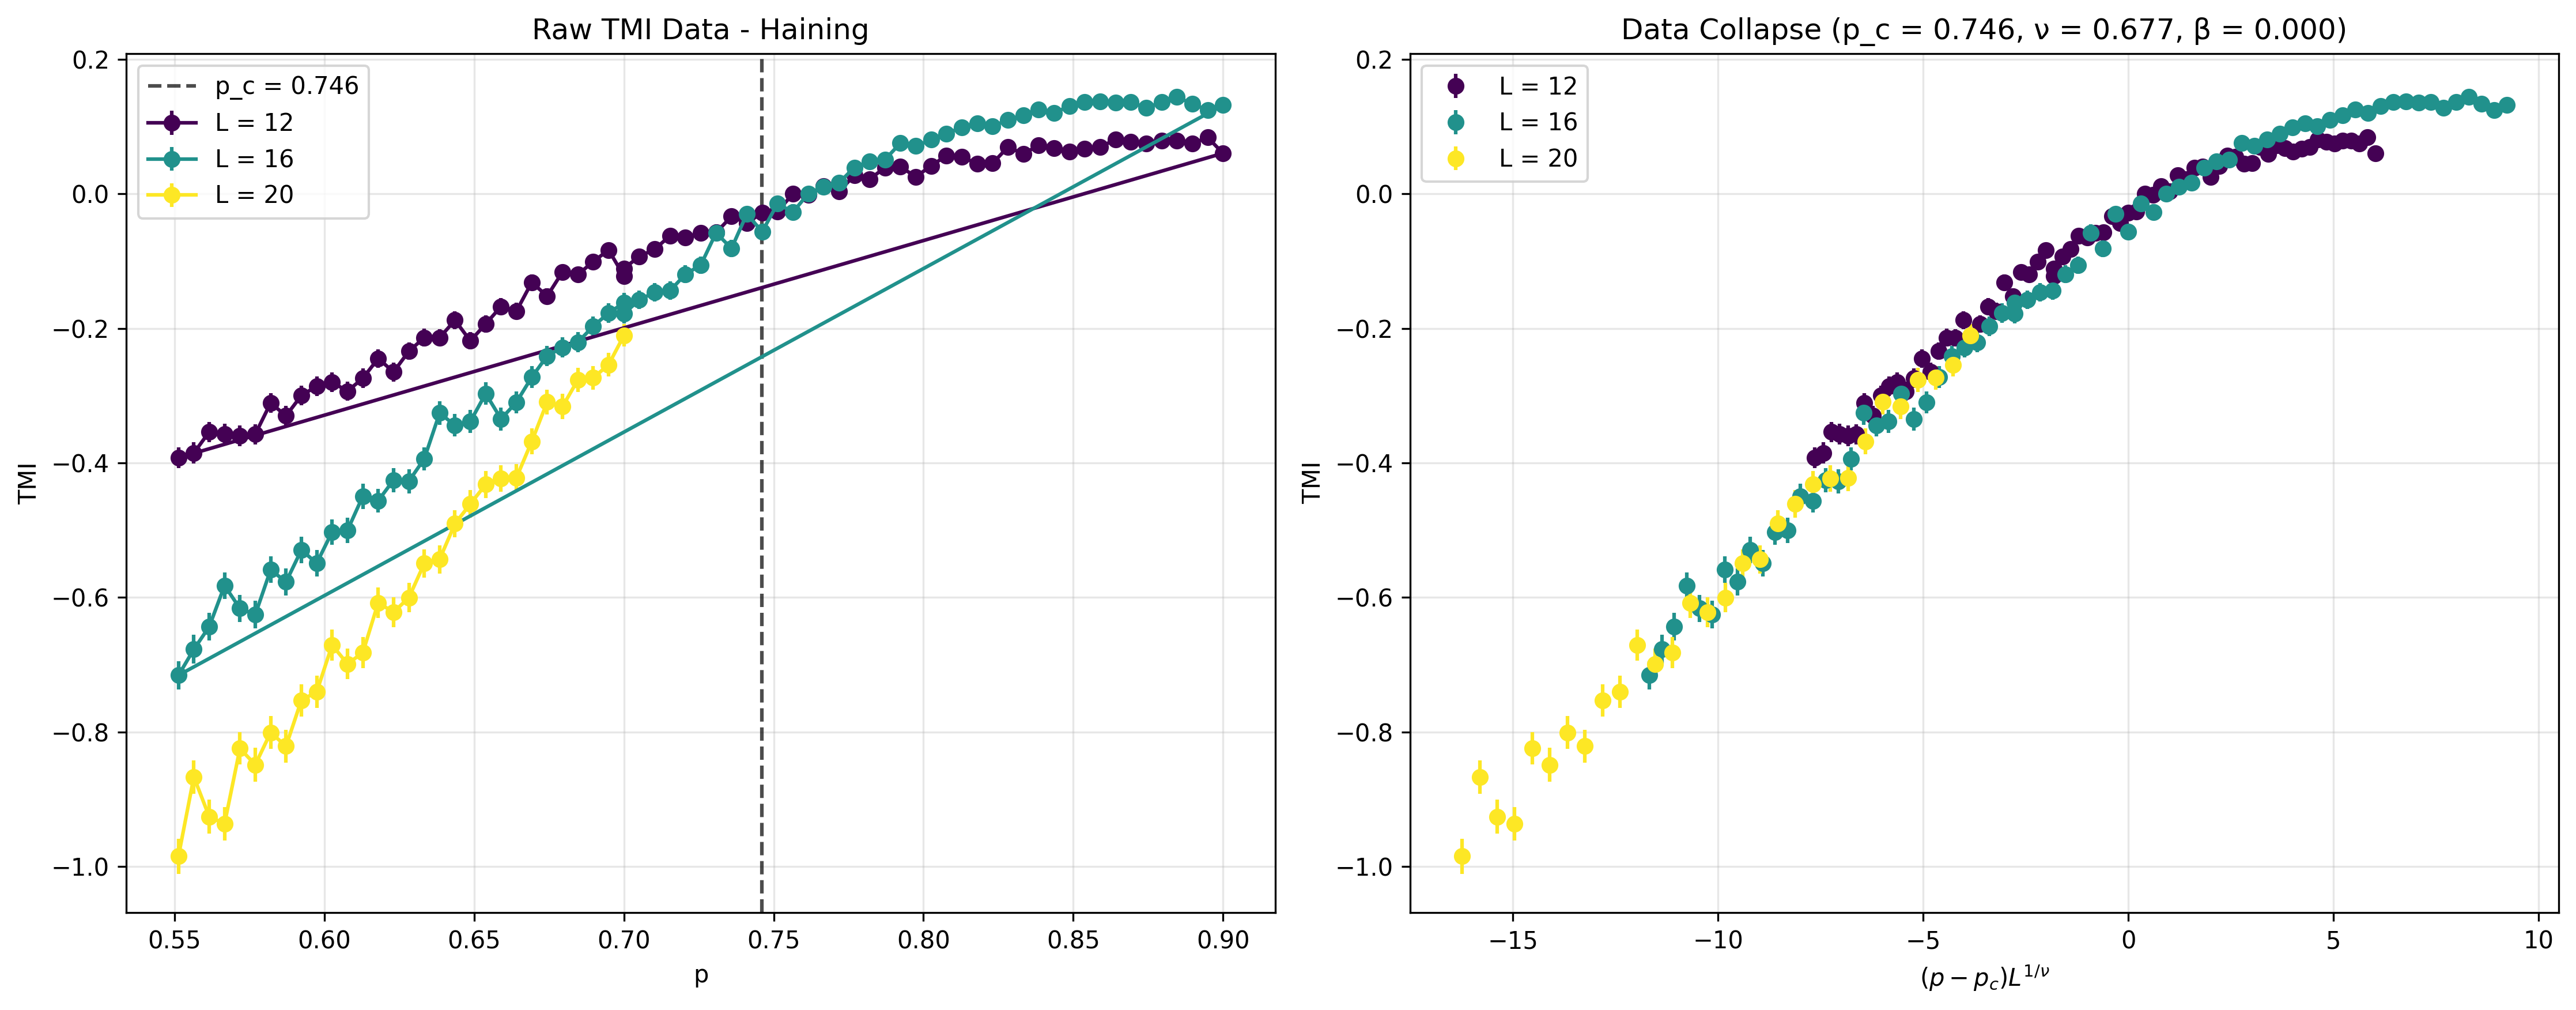
\includegraphics[width=\linewidth]{data_collapse_haining_pctrl0.400_threshold1.0e-15.png}
        \caption{FSS analysis with Haining's codebase.}
        \label{fig:fss_analysis_haining_pctrl0.400}
    \end{subfigure}
    \caption{FSS analysis of the control transition for the global adder with control rate $p_\text{ctrl}=0.4$.}
    \label{fig:fss_analysis_combined_pctrl0.400}
\end{figure}

The developed codebase successfully reproduces both the critical point $p_c=0.75$ and dynamical exponent $\nu=0.7$. Additional analysis includes contour plots (Figure \ref{fig:chi2_contour_pctrl0.400}) and threshold dependence studies (Figures \ref{fig:threshold_dependence_combined_pctrl0.400} and \ref{fig:low_loss_points_combined_pctrl0.400}).

\begin{figure}[H]
    \centering
    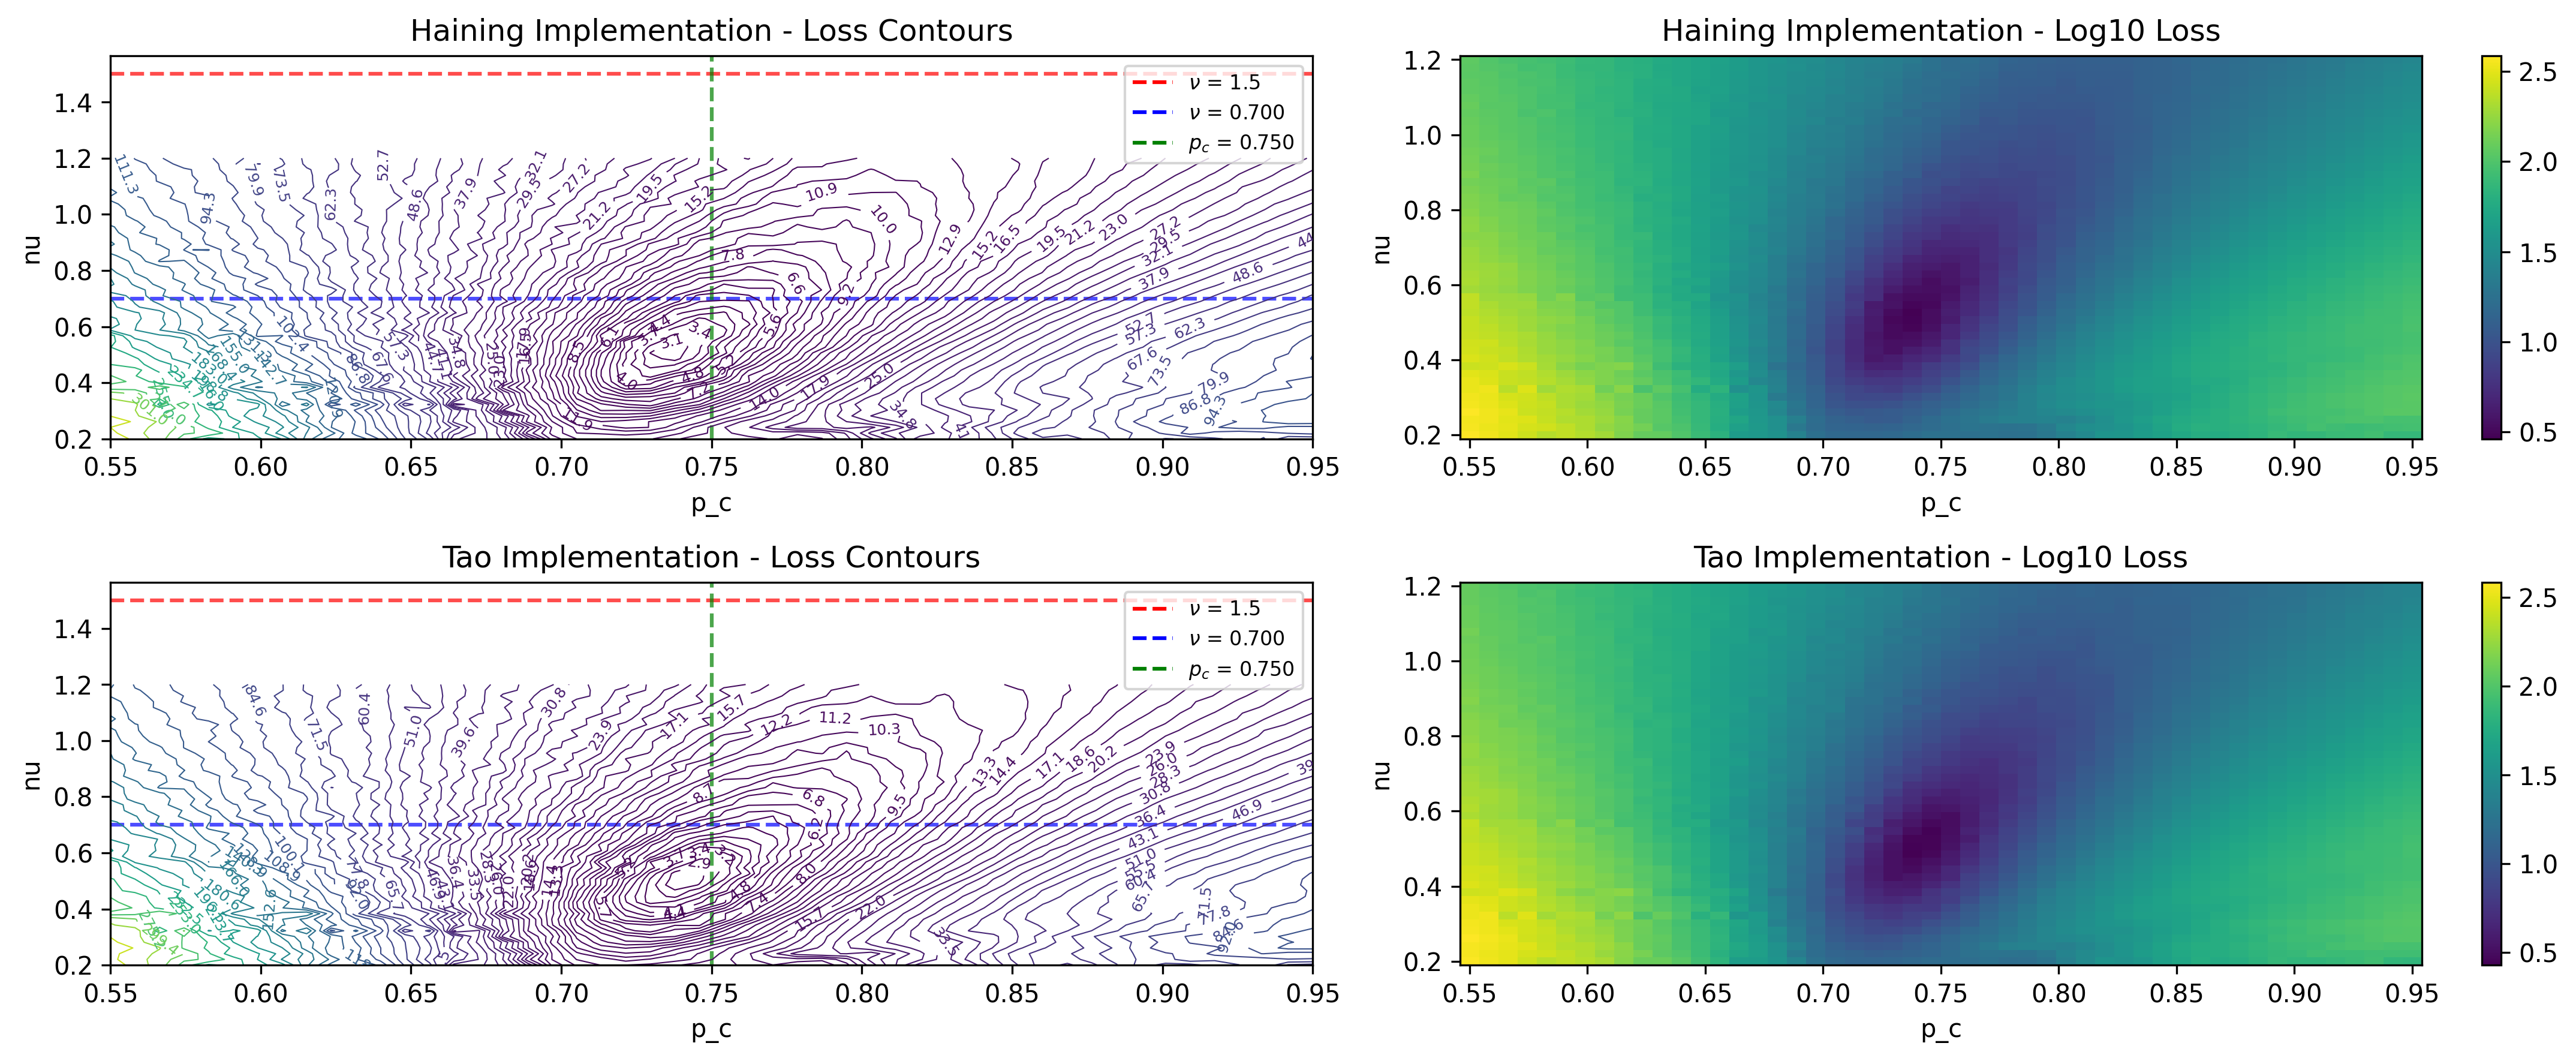
\includegraphics[width=0.8\linewidth]{loss_manifold_comparison_pctrl0.400_threshold1.0e-15.png}
    \caption{Contour of the loss function $\chi^2$ as a function of $p_c$ and $\nu$ for $p_\text{ctrl}=0.4$.}
    \label{fig:chi2_contour_pctrl0.400}
\end{figure}

\begin{figure}[H]
    \centering
    \begin{subfigure}[t]{0.48\linewidth}
        \centering
        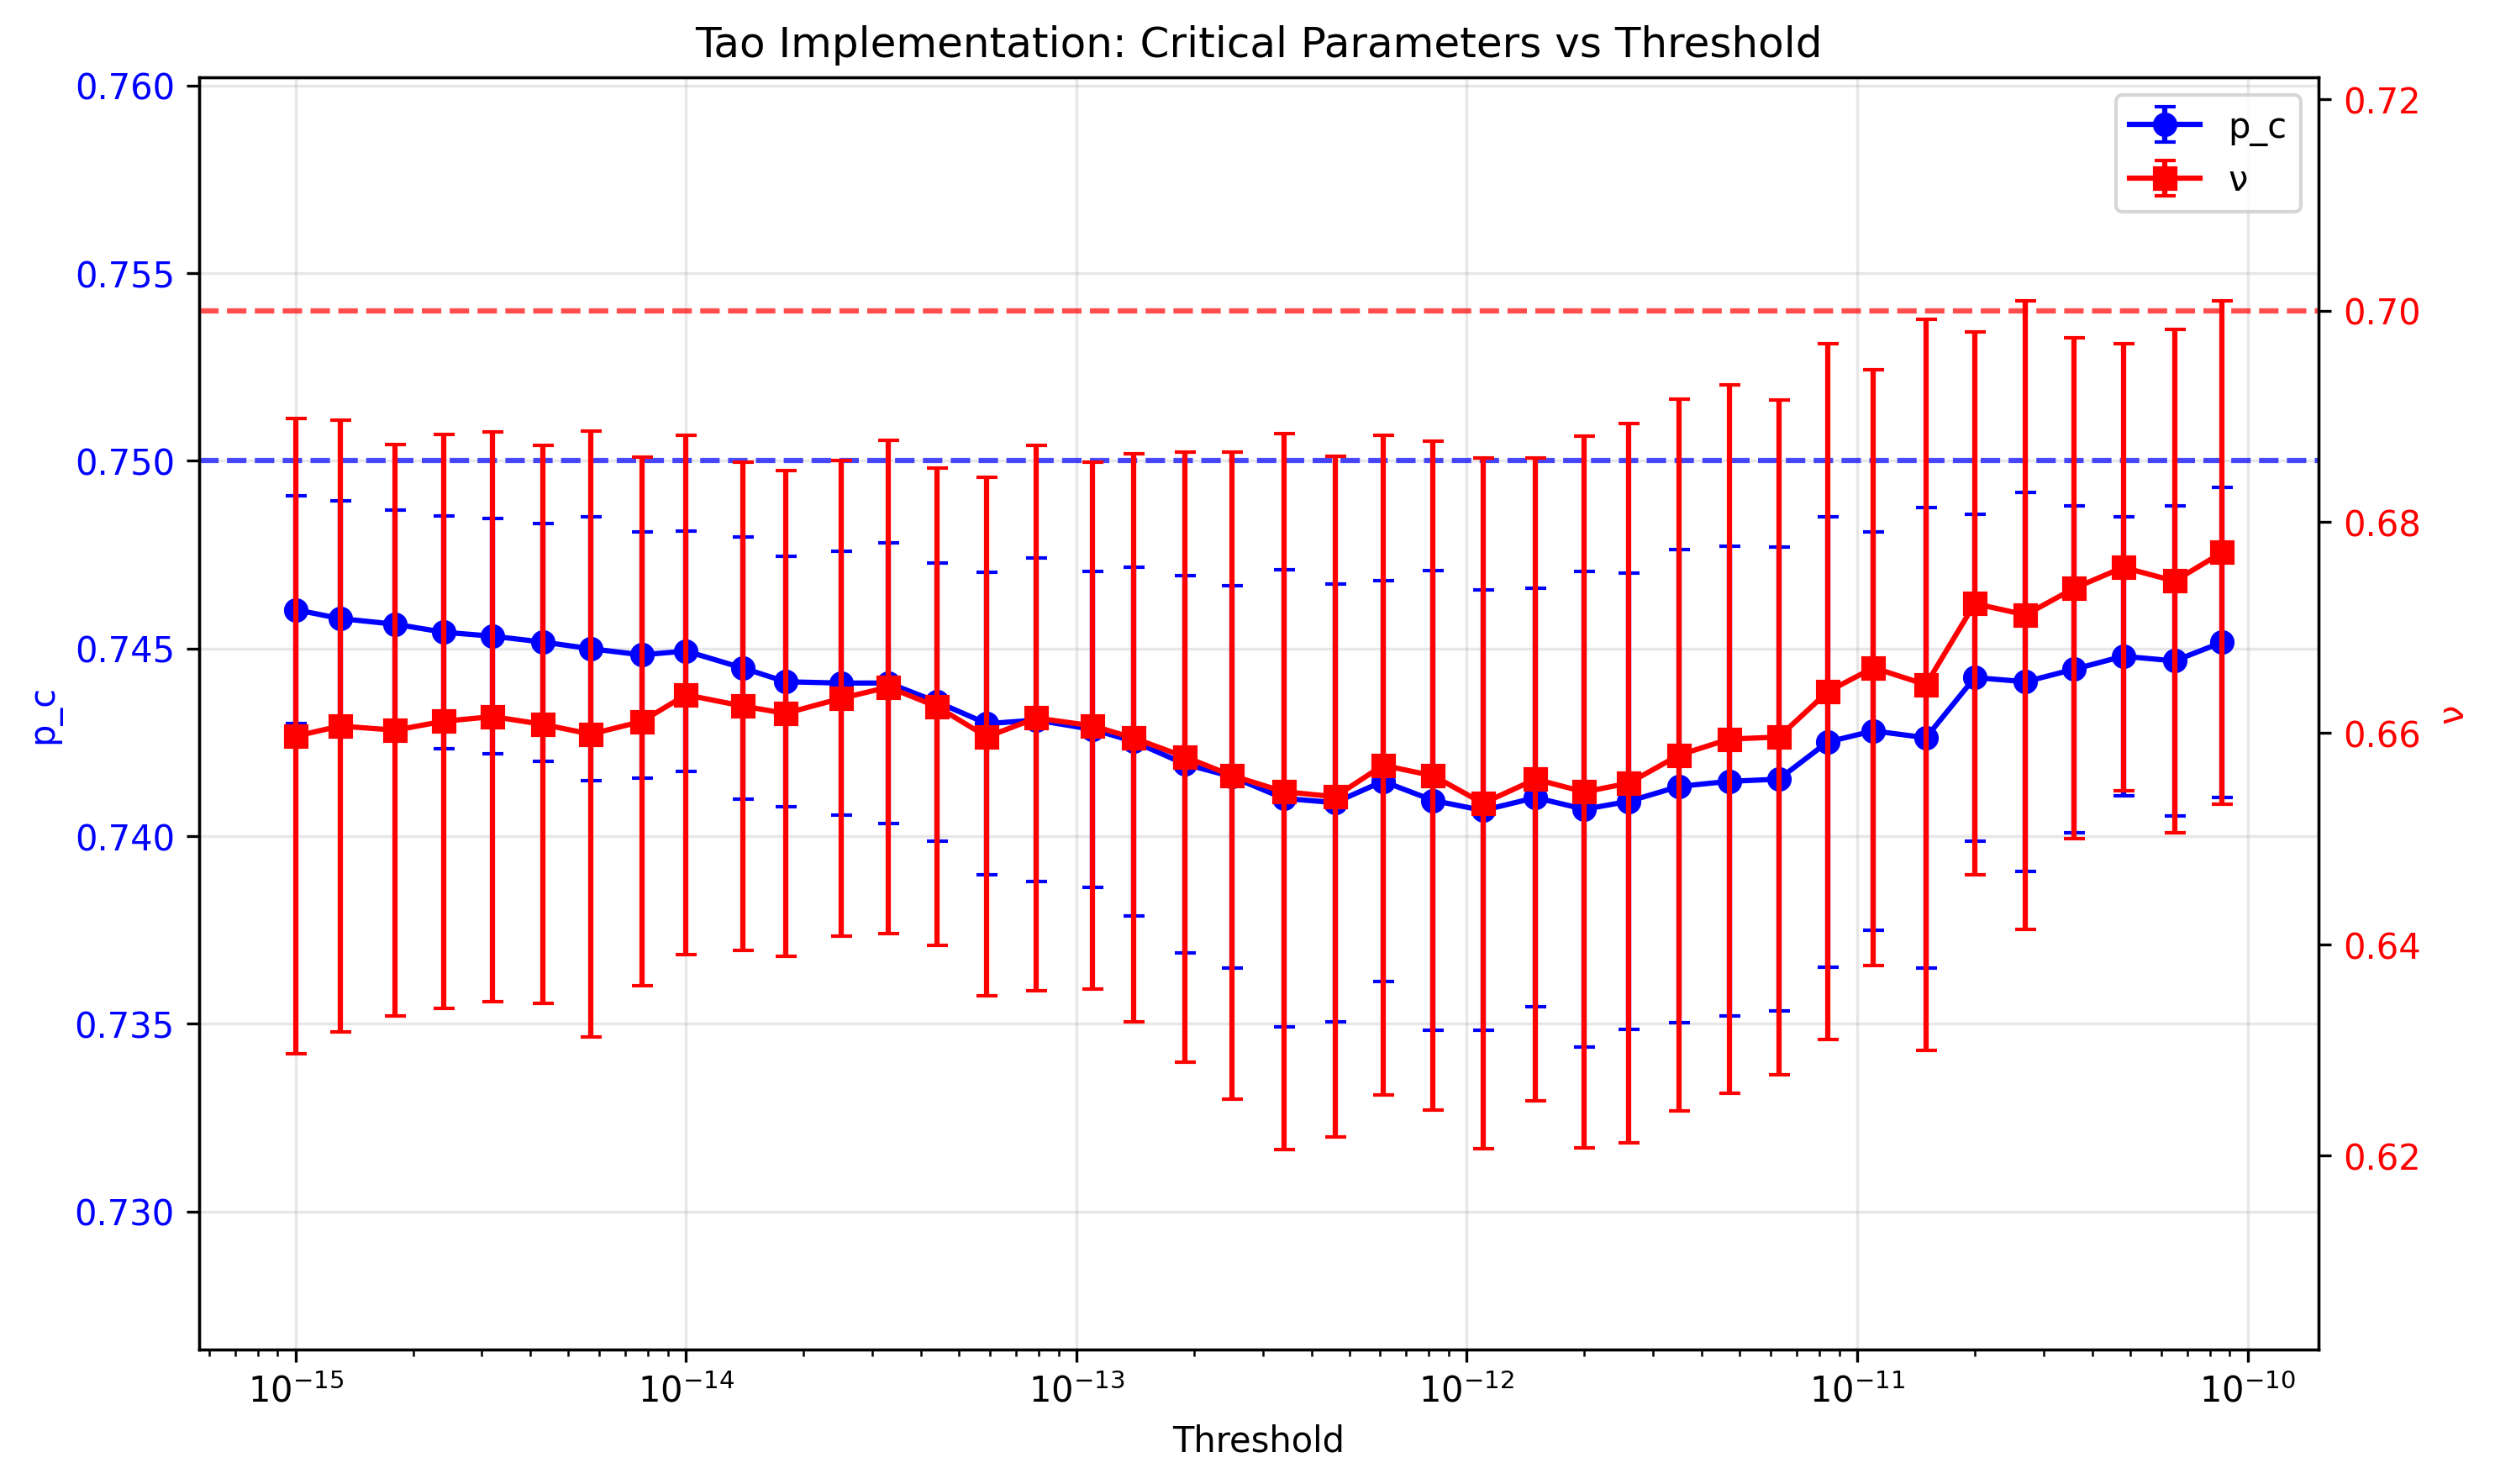
\includegraphics[width=\linewidth]{threshold_dependence_tao_pctrl0.4.png}
        \caption{Threshold dependence with developed codebase.}
        \label{fig:threshold_dependence_developed_pctrl0.400}
    \end{subfigure}
    \hfill
    \begin{subfigure}[t]{0.48\linewidth}
        \centering
        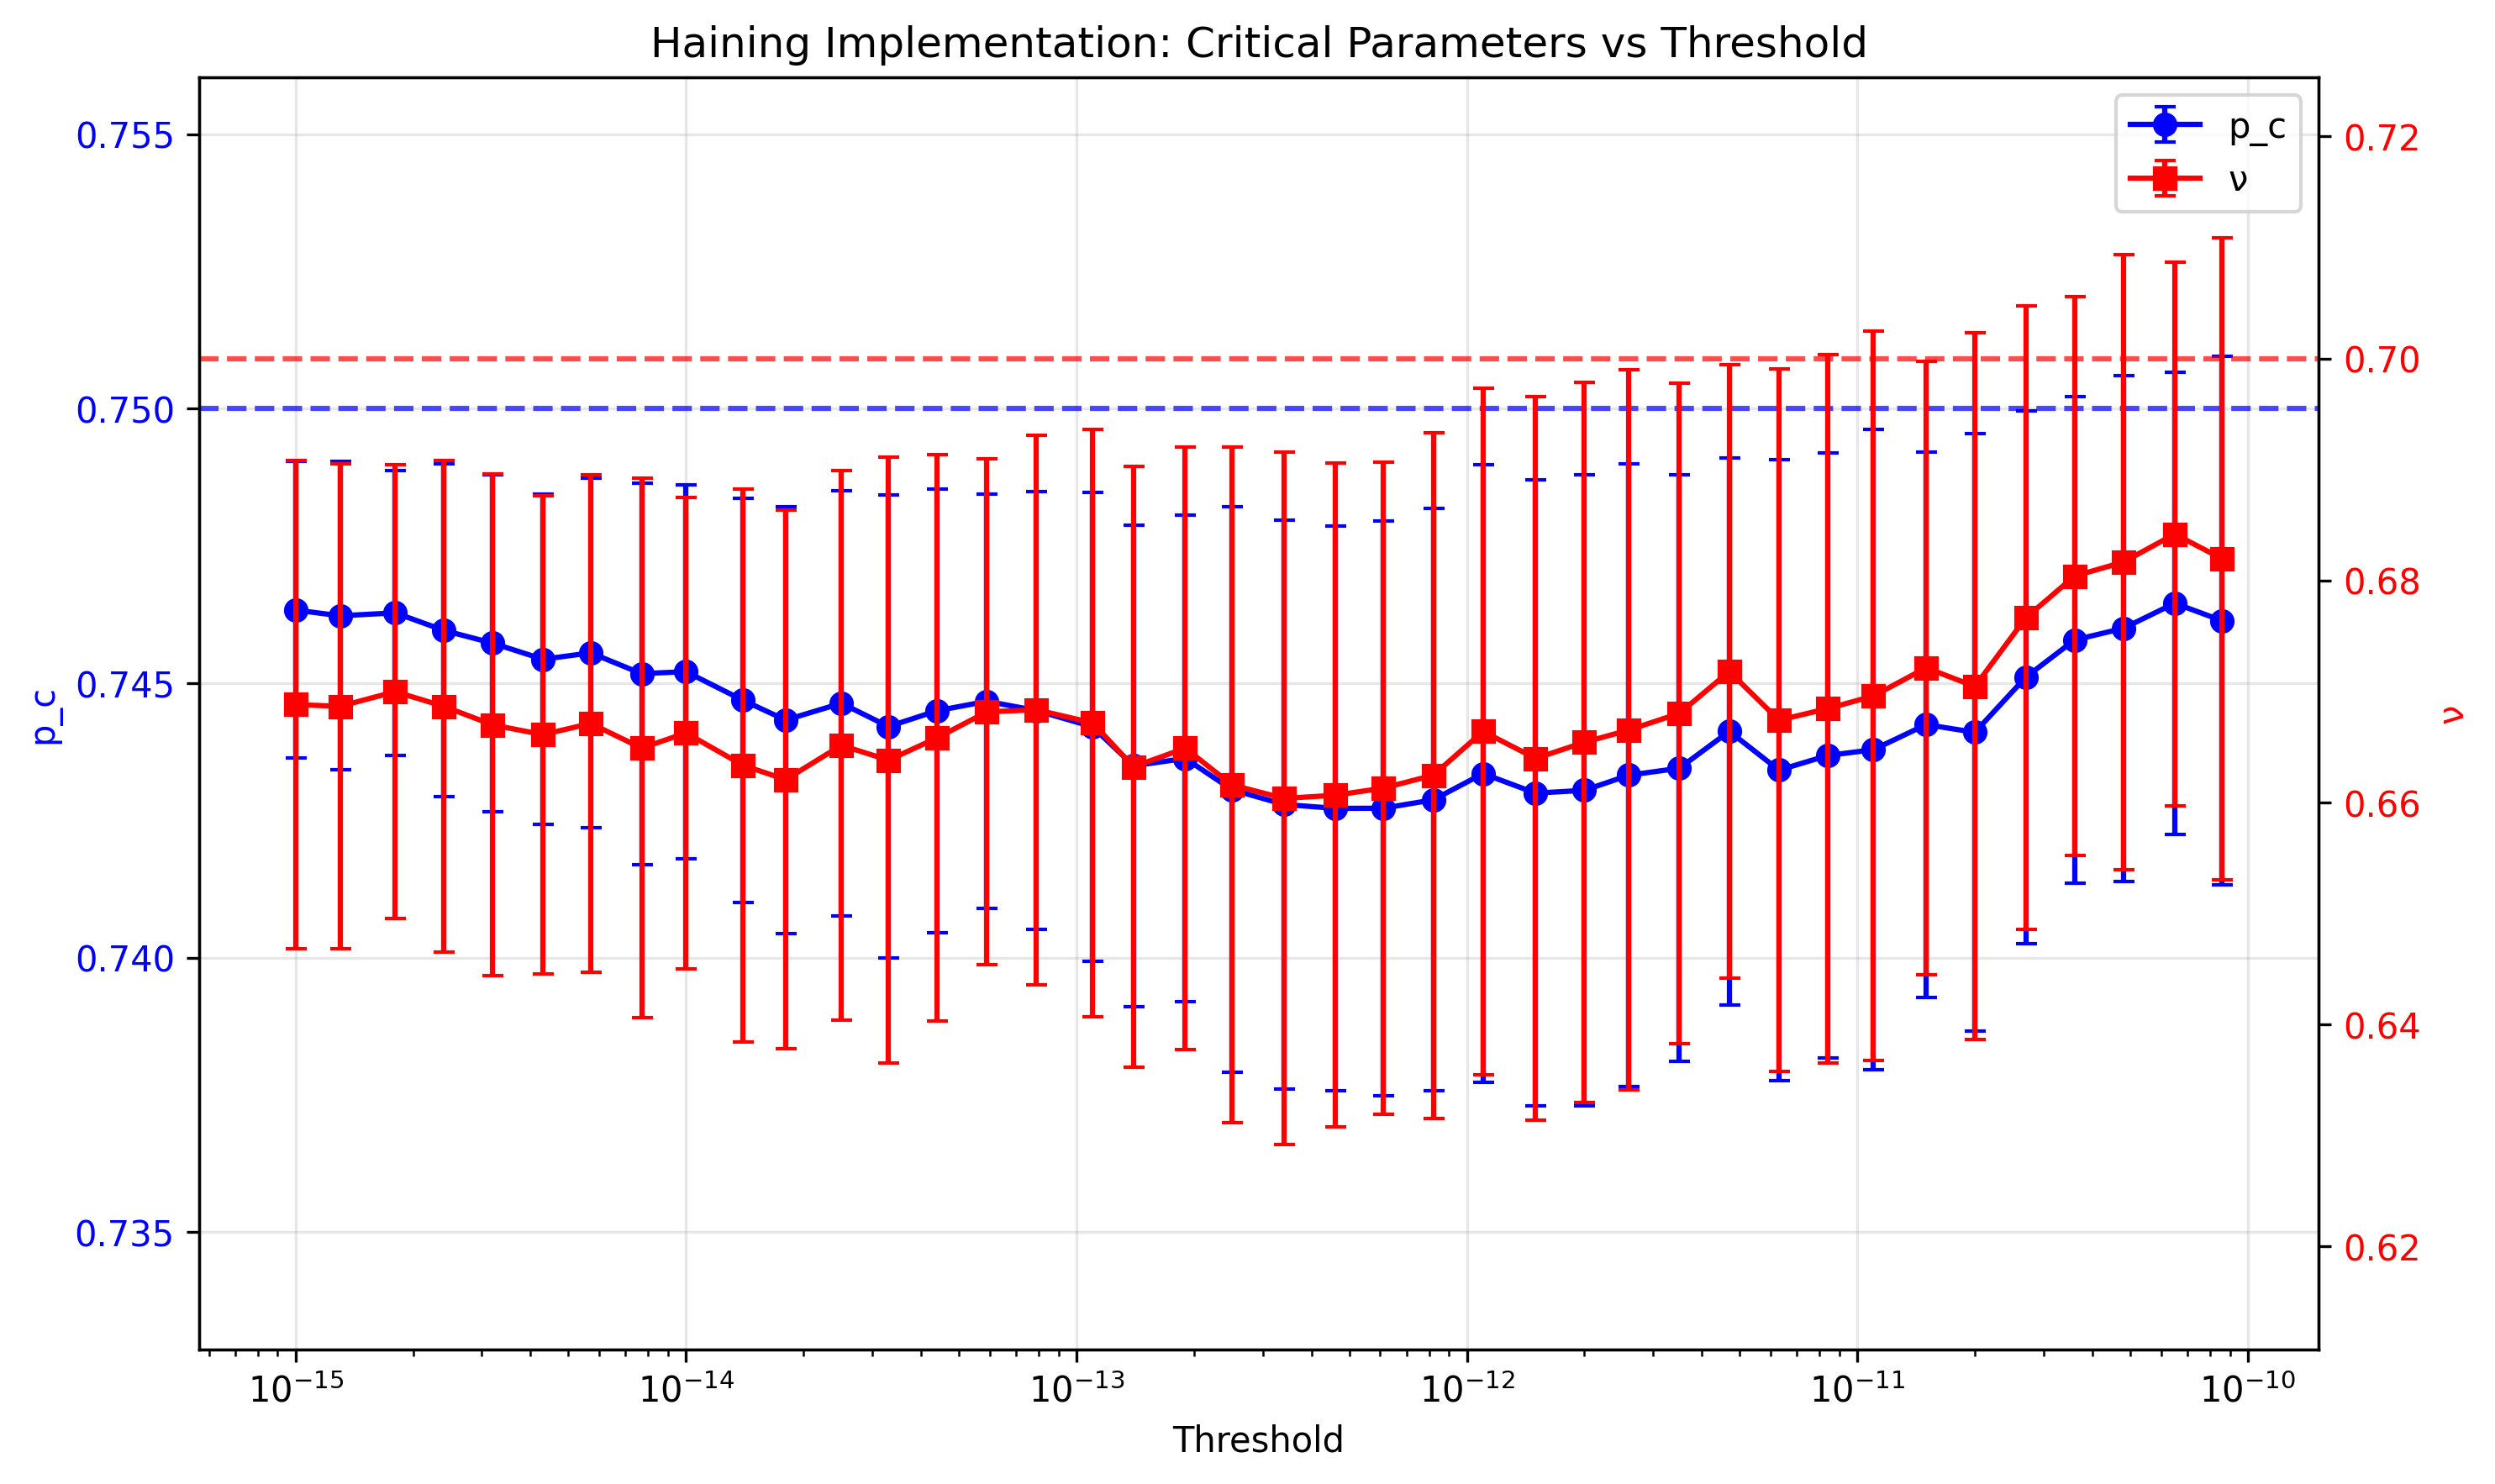
\includegraphics[width=\linewidth]{threshold_dependence_haining_pctrl0.4.png}
        \caption{Threshold dependence with Haining's codebase.}
        \label{fig:threshold_dependence_haining_pctrl0.400}
    \end{subfigure}
    \caption{Threshold dependence of FSS analysis for $p_\text{ctrl}=0.4$.}
    \label{fig:threshold_dependence_combined_pctrl0.400}
\end{figure}

\begin{figure}[H]
    \centering
    \begin{subfigure}[t]{0.8\linewidth}
        \centering
        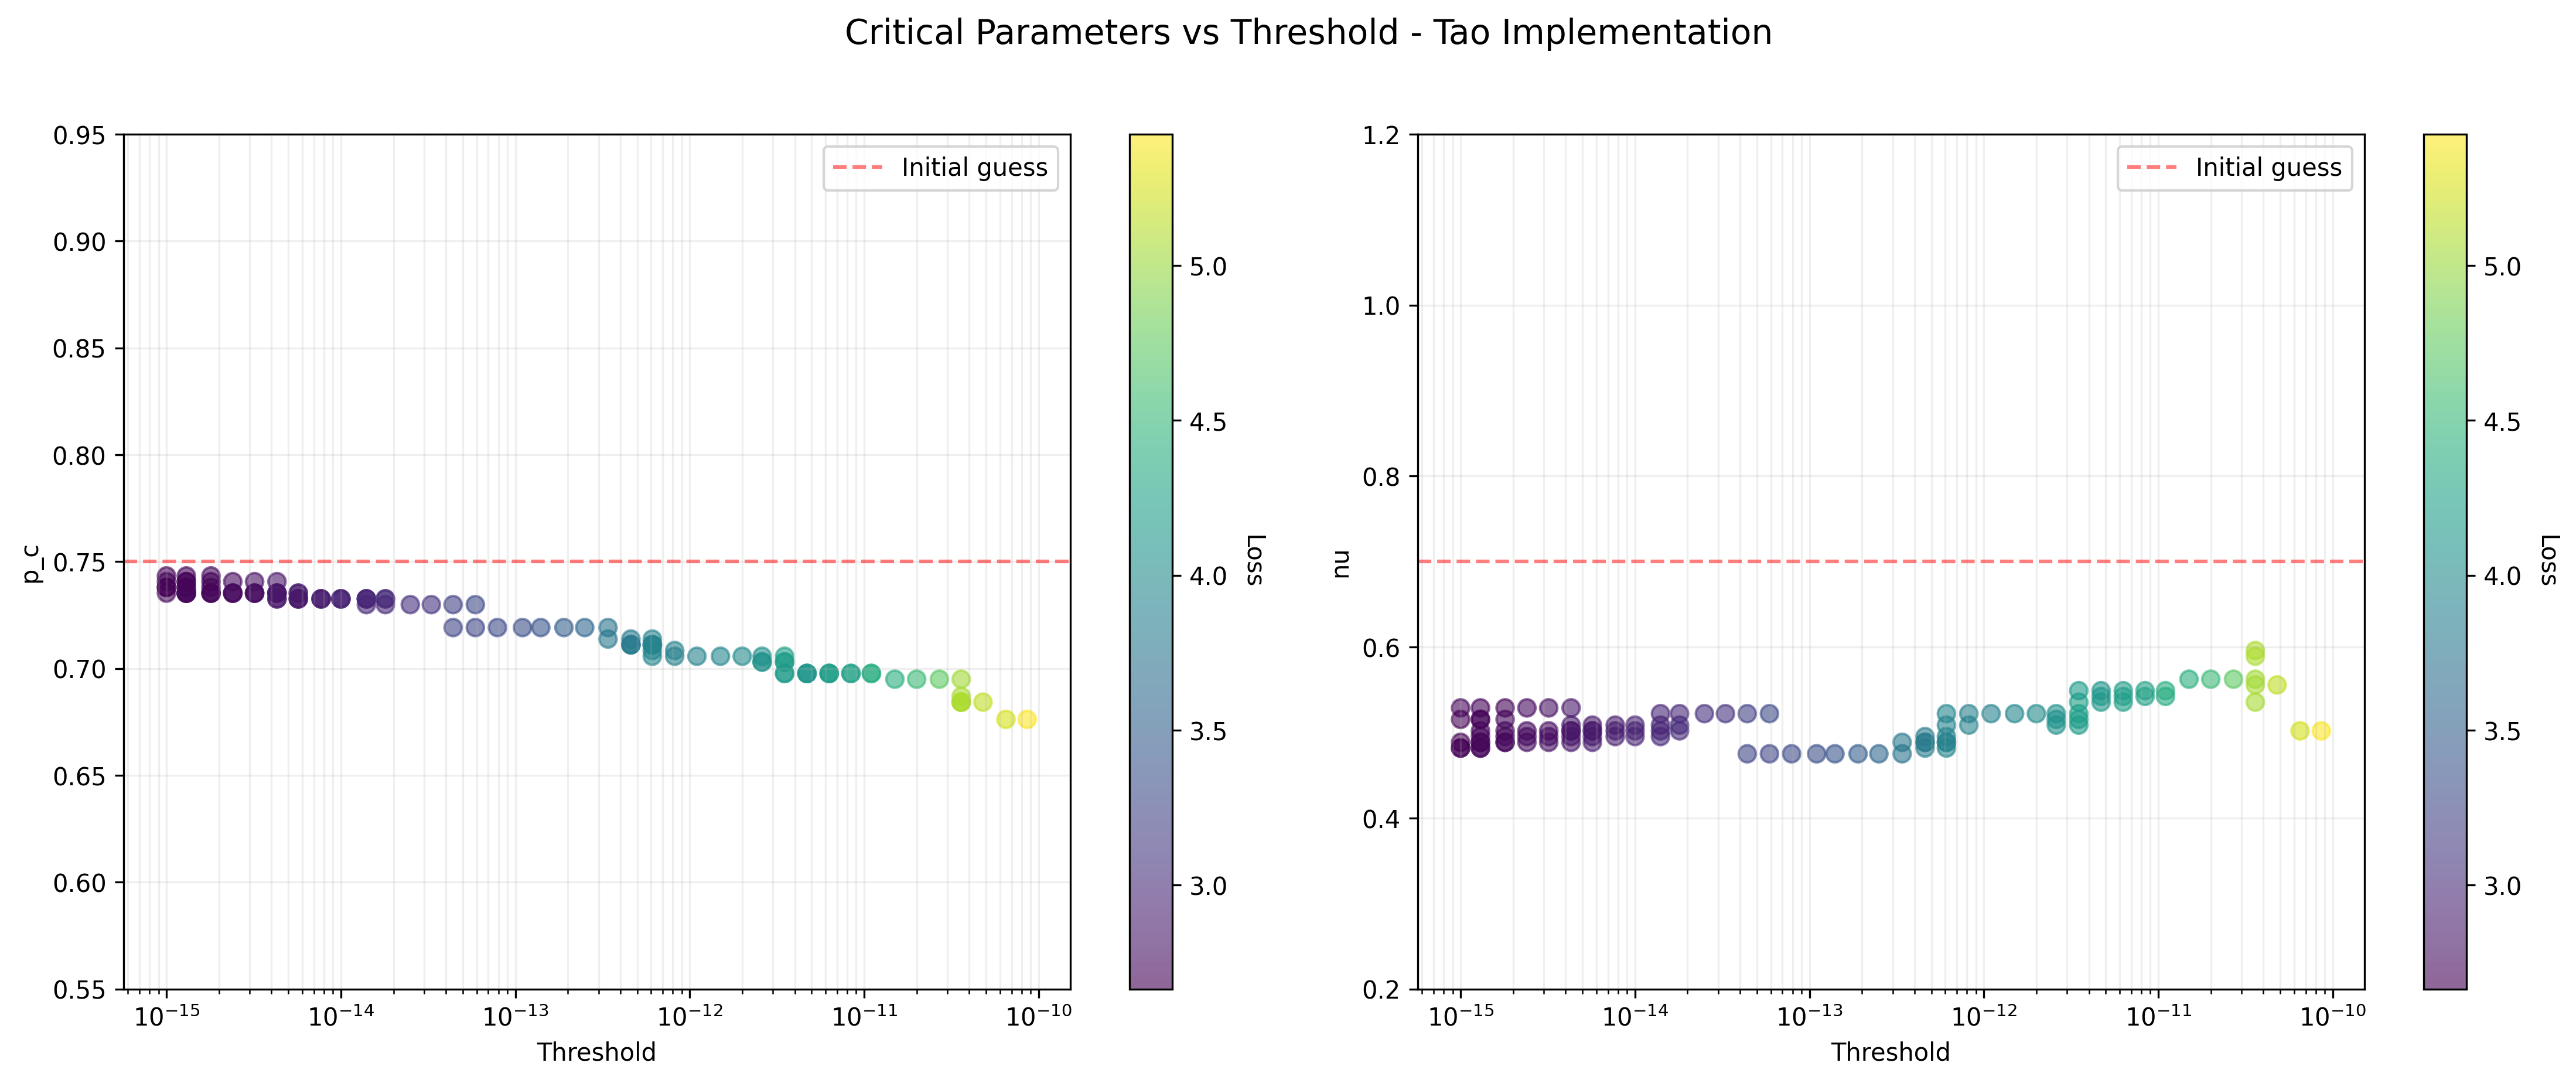
\includegraphics[width=\linewidth]{threshold_dependence_pctrl0.400_tao.png}
        \caption{Low loss points with developed codebase.}
    \end{subfigure}
    \vfill
    \begin{subfigure}[b]{0.8\linewidth}
        \centering
        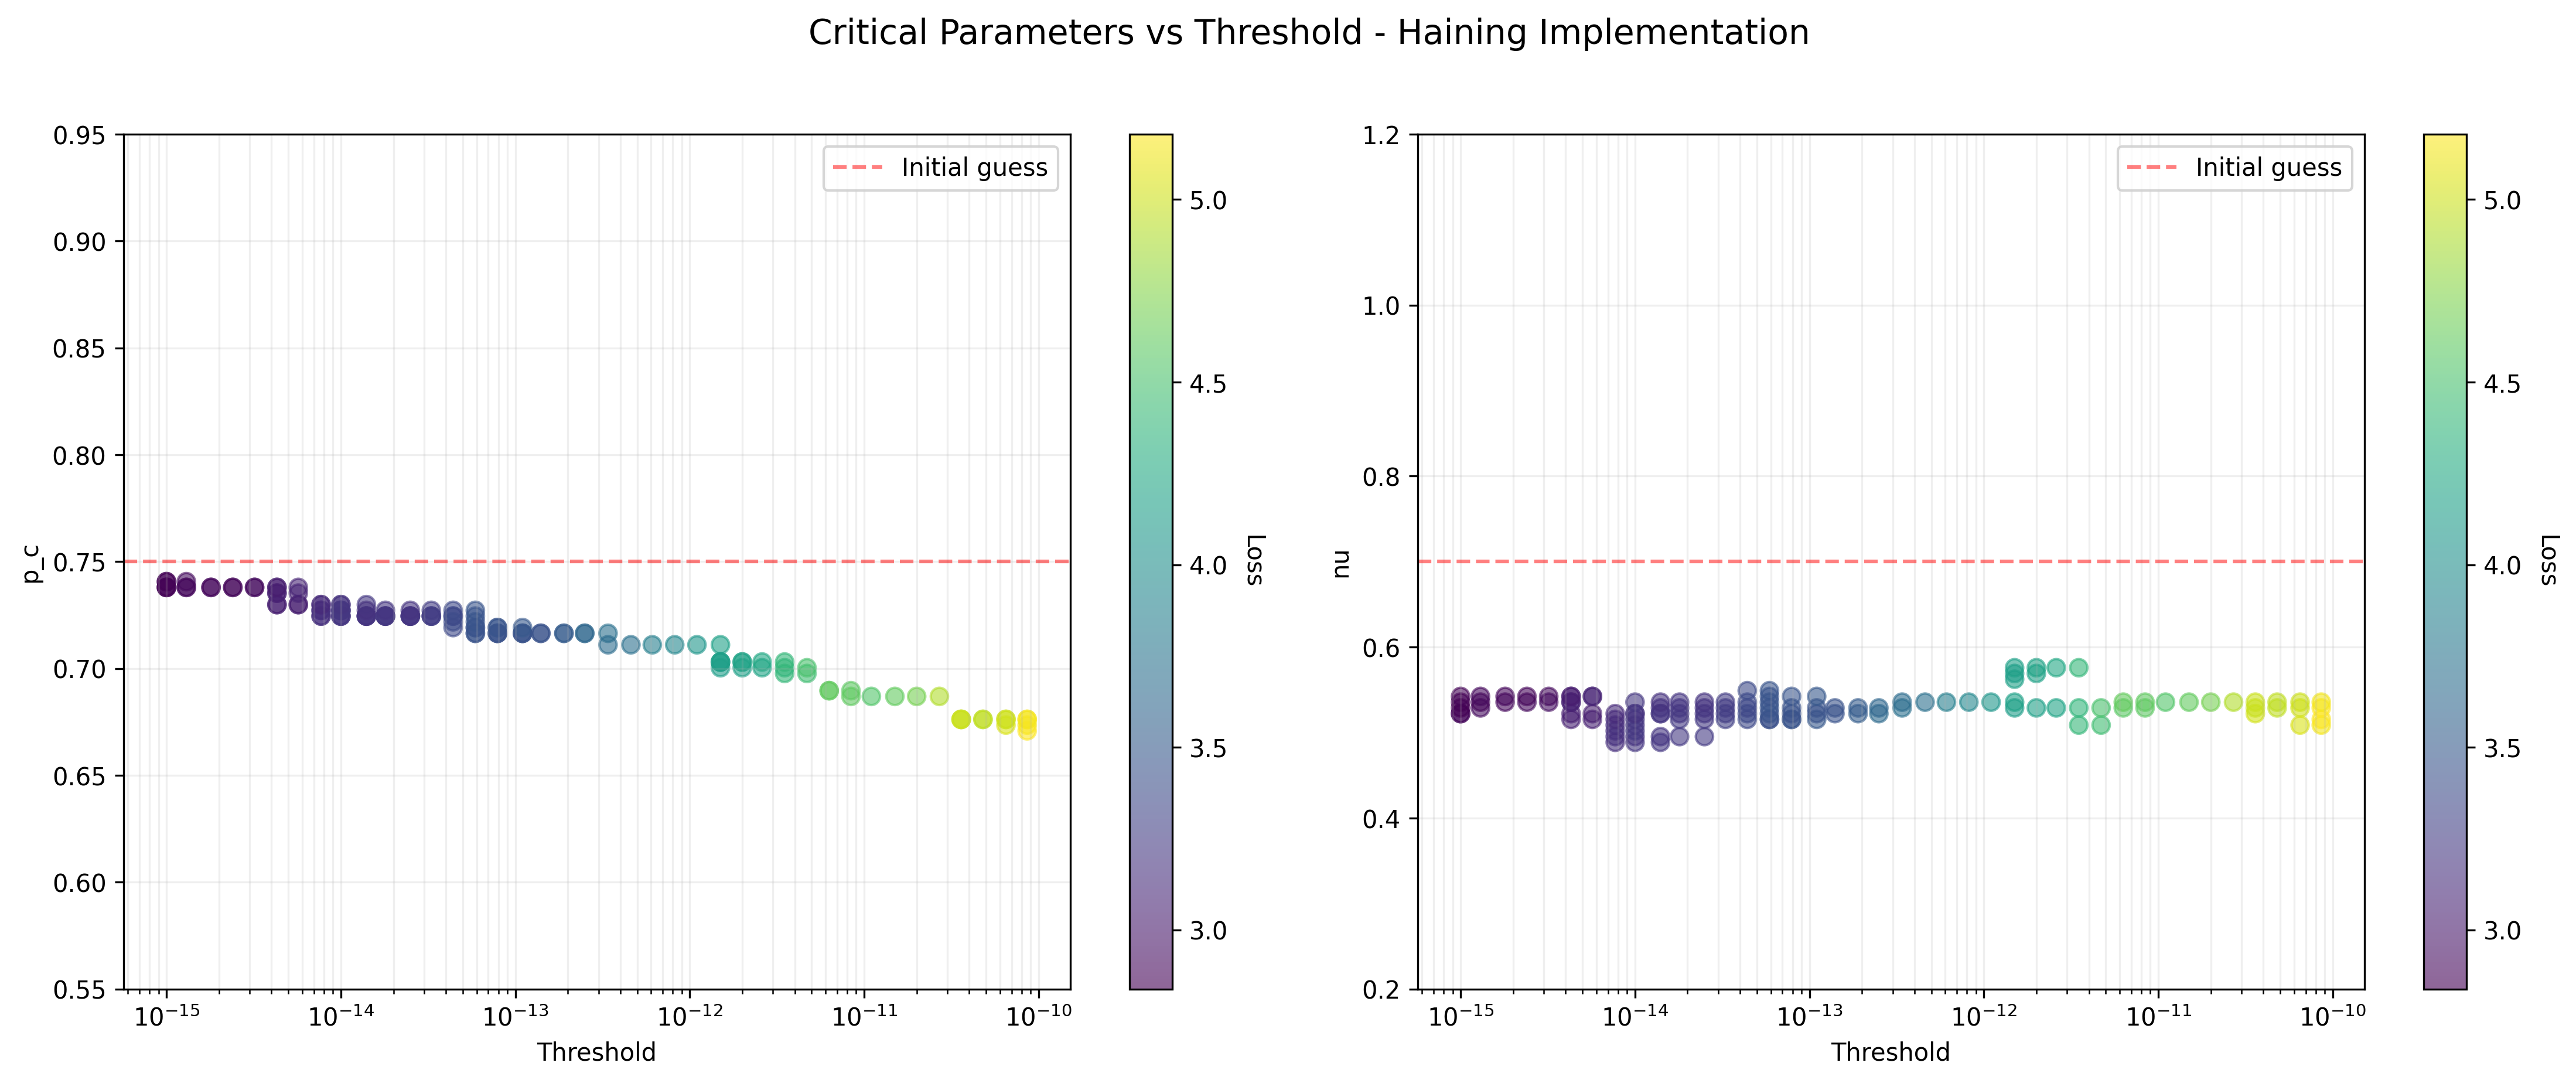
\includegraphics[width=\linewidth]{threshold_dependence_pctrl0.400_haining.png}
        \caption{Low loss points with Haining's codebase.}
    \end{subfigure}
    \caption{Low loss points from FSS analysis for $p_\text{ctrl}=0.4$.}
    \label{fig:low_loss_points_combined_pctrl0.400}
\end{figure}

\subsection{Initial Phase Summary}

The developed codebase successfully reproduces both critical points ($p_c$) and dynamical exponents ($\nu$) from published results. While numerical fluctuations exist in the analysis, they appear to be computational artifacts rather than fundamental physics implementation issues. The results demonstrate thorough understanding of the Bernoulli control transition, providing a solid foundation for advancing to the second phase: implementing the control transition using Matrix Product States (MPS). The MPS formalism will enable investigation of larger system sizes and significantly increased sample numbers, improving precision and enabling exploration of previously inaccessible parameter regimes.

\section{Question for Haining (April 20, 2025)}

A discrepancy has been identified between the theoretical paper and the codebase implementation regarding the order of operations for control and Bernoulli maps.

According to the paper, the control map operation sequence should be: measure and reset the last qubit, translate to the right, then apply the adder. For the Bernoulli map, the sequence should be: left translation first, then apply the random unitary.

However, the codebase implementation appears to follow a different sequence. For the control map: measure and reset the last qubit, apply the adder, then translate the lattice to the left (not right). For the Bernoulli map: apply the random unitary on the last two qubits, then translate to the right (not left).

If the codebase is correct, there must be an index shifting step that requires investigation. A detailed analysis of the function S! is needed to understand how the MPOs are applied to the MPS.

\begin{lstlisting}
if rand(ct.rng_C) < p_ctrl
    # control map
    if ct.xj in Set([Set([1 // 3, 2 // 3]),Set([0])])
        p_0= inner_prob(ct, [0], [i])
        n =  rand(ct.rng_m) < p_0 ?  0 : 1
        control_map(ct, [n], [i])
        push!(op_l,Dict("Type"=>"Control","Site"=>[i],"Outcome"=>[n]))
    end
    # Currently: Measure+reset -> adder -> LEFT translation (does the order not matter here?)
    i=mod(((i-1) - 1),(ct.L)) + 1  # LEFT translation
else
    # Bernoulli map
    Bernoulli_map!(ct, i)
    push!(op_l,Dict("Type"=>"Bernoulli","Site"=>[i,((i+1) - 1)%(ct.L) + 1],"Outcome"=>nothing))
    # Currently: Apply unitary -> RIGHT translation
    i=mod(((i+1) - 1),(ct.L) )+ 1  # RIGHT translation
\end{lstlisting}

\section{Task List (April 24, 2025)}

\begin{enumerate}
    \item Determine procedures for performing measurements on the cluster machine
    \item Learn GPU usage for local development
    \item Learn GPU usage on the cluster environment
\end{enumerate}

\section{Task List (April 28, 2025)}

\begin{enumerate}
    \item Perform von Neumann entropy calculations on the cluster. Since access to the OSG cluster is unavailable, new shell scripts must be created to run the code on Amarel through SLURM.
\end{enumerate}

\section{Task List (May 2, 2025)}

\begin{enumerate}
    \item Set up \texttt{run\_CT\_MPS} on the Amarel cluster using Singularity
\end{enumerate}

Singularity functions similarly to WSL2 by providing virtual operating systems that ensure software is installed with correct version dependencies. The strategy involves downloading .def files for Julia from DockerHub to establish appropriate Docker images on Amarel.

\section{Issue (May 21, 2025)}

File copy error encountered: \texttt{\%file cannot copy src CT.jl into /tmp/julia\_env/CT/}

\section{Issue (May 22, 2025)}

Investigation revealed that Julia packages are stored in \texttt{tmp/julia\_env/CT/} locally, which explains the persistent CT references in tmp. The primary issue is that tmp directories are not writable in Apptainer environments.

An additional complication was discovered: duplicate TOML files exist - one in CT (created by Haining) and another in \texttt{tmp/julia\_env/CT} (created by the user). After updating Haining's TOML project files for consistency with CT, testing was conducted to verify that example scripts can run in the Apptainer environment. Upon successful testing, the duplicate TOML files were deleted.

With duplicate TOML files removed and only working versions of CT remaining, the procedure for transferring to the Amarel cluster was established:
\begin{enumerate}
    \item Create a new folder on the server
    \item SCP the necessary folders ("CT" and .jl scripts) along with the .def files
    \item Set up Apptainer with the correct Julia version
    \item Instantiate the CT project using the TOML files
    \item Perform a test run using SLURM
    \item If successful, begin the parallelization process
\end{enumerate}

The Singularity container \texttt{julia\_itensor.sif} was successfully built with all packages precompiled, including CT. The next objectives are: (1) modify \texttt{run\_CT\_MPS\_1-3.jl} for late-time computation over many different realizations, and (2) write the parallelization shell script for execution with sbatch.

\section{Issue (May 23, 2025)}

Parallelization implementation has been completed. However, a significant performance issue has emerged: Julia execution times are excessively long, even for small systems such as L=8. Consultation with Haining is needed to determine if additional caching for optimization is required.

\section{Issue (May 25, 2025)}

Investigation into the Julia codebase performance issue has begun. Initial testing involves conducting a local run of L=8 to measure execution time, which should be compared against Haining's benchmark of 0.8 seconds.

\textbf{Performance Analysis:}

The main loop execution time is significantly longer than expected. The target time should be approximately 0.6-0.8 seconds, but current measurements show 26 seconds. During single-shot main loop testing, an interesting pattern emerged: the first two runs take abnormally long (~26s), but all subsequent runs execute extremely fast (~0.07s).

\textbf{Factors that can trigger recompilation:}
Changes in type parameters or function signatures, modifications to method definitions, changes in the dependency chain of functions, using different types as arguments than previously compiled, modifications to custom package code (such as the CT package), loading new packages that extend or modify existing methods, and changes in global constants that affect method specialization.

\textbf{Analysis of precompiled packages:}
The .sif container contains .ji Julia cache files for each package, representing shallow compilation that prepares the basic package structure. When Julia uses these files, packages load faster, but this does not mean the actual function code for specific types is utilized. Cached files in .sif containers serve as maps for Julia to create binaries faster, but the binaries are not directly present, resulting in overhead. This is why system images (.so or .dylib files) are also needed - they contain full binaries with compiled machine code (deep compilation).

\textbf{System image testing:}
Initial attempts to create system images to eliminate overhead before packaging into .sif were conducted. Using the existing system image, the main loop still required 17 seconds, suggesting that not all essential functions were precompiled into binary format.

The most recent attempt successfully built the system image. Testing L=8 with the system image reduced the first run time from 17 seconds to 2 seconds, with subsequent JIT runtime remaining at 0.08 seconds. The remaining time difference is attributed to runtime compilation that cannot be eliminated through precompilation.

The next steps involve: (1) including the system image building process within Apptainer to build the .sif file, (2) testing single-shot runs with the .sif file on the cluster to achieve the target 2-second performance, and (3) investigating further performance improvements through JIT warmup.

Container testing achieved the required ~2-second performance (with the minor issue of container size reaching 1.7GB). Uploading the new .sif file to the cluster for testing required the following files: \texttt{julia\_itensor.sif} and \texttt{run\_CT\_MPS\_1-3.jl}.

Cluster testing was successful: single-shot runs under .sif take approximately 4 seconds for the first execution and 0.1 seconds for subsequent runs. This performance can be improved by precompiling additional packages into the system image binary file.

\textbf{Precompilation Instructions:}

Julia can only precompile packages, not scripts directly. The recommended approach follows this example:

\begin{lstlisting}
# precompile.jl
using CT, ArgParse
include("run_CT_MPS_C_m_T.jl")
# do one dummy call so all methods get JIT'ed
main_interactive(10, 0.1, 0.2, 1, 1)
 
# To run the precompilation, use the following command:
# export JULIA_DEPOT_PATH=~/julia_depot
# export TMPDIR="/tmp" # (optional)
# using PackageCompiler; using Pkg; Pkg.activate("CT")
# create_sysimage(
#     [:CT, :ITensors, :ArgParse, :JSON, :MKL],
#     sysimage_path="ct_with_wrapper.so",
#     precompile_execution_file="precompile.jl"
#   )
 
 
# Then to start from the sysimage, use:
# julia --sysimage ct_with_wrapper.so --project=.
# > using Pkg
# > Pkg.activate("CT")
# > main_interactive(8, 0.1, 0.2, 1, 1)
#
# Or call the script directly:
# julia --sysimage ct_with_wrapper.so \
#       --project=. \
#       -p 4 \
#       run_CT_MPS_C_m_T_multiproc.jl \
#       --params "0.5,0.0,8,1,1,0.5,0.0,8,2,2"
 
 
For generic compilation
create_sysimage(
    [:CT, :ITensors, :ArgParse, :JSON, :MKL],
    sysimage_path="run_CT_MPS_evo_generic.so",
    precompile_execution_file="precompile_evo.jl",
    cpu_target="generic;skylake-avx512,clone_all;znver2,clone_all"
  )
\end{lstlisting}

The reference implementation \texttt{run\_CT\_MPS\_C\_m\_T\_multiproc.jl} can be found in the GitHub repository.

\textbf{Additional considerations:} Investigation into memory statistics and backend implementation could provide valuable insights into system structure.

\section{Issue (May 26, 2025)}

Testing with .sif files containing all precompiled packages still failed to achieve the target initial run time of 0.6 seconds. Potential causes include: (1) different calculation procedures between scripts, and (2) since CT was already precompiled in previous runs and the .jl script primarily uses CT, no significant speedup was observed.

Testing should be conducted with the same script (\texttt{run\_CT\_MPS\_C\_m\_T.jl}) before concluding whether precompilation was implemented correctly.

Results from testing with \texttt{run\_CT\_MPS\_C\_m\_T} still failed to achieve the 0.6-second target. The current best performance is 10 seconds initial and 1 second subsequent execution. Further investigation of Haining's code is required.

Modifications were made to the .def build process and \texttt{create\_sysimage\_ct} to include the entire \texttt{run\_CT\_MPS\_C\_m\_T} file and its \texttt{main\_interactive()} function to pursue performance improvements. Additionally, the reason for setting \texttt{num\_julia\_threads = 2} requires clarification.

Test results showed: local runtime of 7 seconds initial and 1.5 seconds subsequent. Interactive Singularity shell runs on the cluster demonstrated 1.4 seconds initial and 1 second for subsequent executions.

It may be worthwhile to examine Haining's codebase and test the \texttt{run\_CT\_MPS\_C\_m\_T\_multiproc} function to identify differences.

Before implementing parallel processing on the cluster, investigating whether precompilation is possible after container construction would be valuable.

\section{Issue (May 27, 2025)}

Difficulties were encountered while operating the container on macOS. During development of helper scripts to run Julia scripts with runtime JIT warmup in the Singularity container, compatibility issues arose with the macOS environment.

To address this, Lima (a macOS virtual environment for Linux) was installed, the entire workspace was migrated to the virtual environment, and Julia and Apptainer were installed within the virtual environment. After initial build difficulties, local testing confirmed that image creation functions properly.

An attempt was made to move the .so file to the appropriate location under .sif to resolve image creation issues. However, this approach failed because the container is a static system, and the content of \texttt{/opt/CT/sysimage} cannot be modified once built.

An alternative approach was adopted: the container contains only necessary packages (without embedded system images). Two options were identified for achieving image speedup:

\begin{enumerate}
    \item Manually specify the desired image using \texttt{julia --sysimage="path/to/sysimage"}
    \item Mount the Singularity container directly to the directory containing the image and run Julia without specifying the system image
\end{enumerate}

This approach allows creation of new .so system images for different .jl files, which can be uploaded and executed using either option.

Local testing confirmed that separating the container and image works effectively. Both components were then uploaded to the cluster for verification.

Cluster testing was successful, enabling implementation of parallelization. The first step involved creating the image file \texttt{run\_CT\_MPS\_ensemble.so}. A testing function \texttt{main\_interactive} was added to pass explicit arguments for JIT warmup and image creation.

The system image integration with the cluster container was successful, and SLURM script testing commenced.

Initial SLURM script execution appeared successful. While awaiting results, workflow documentation and GitHub commits were completed.

\textbf{Side project consideration:} Investigating the possibility of migrating the entire workspace through remote SSH connection via Cursor to the cluster, enabling complete cloud-based development where work sessions involve opening Cursor, SSH connection to the cluster, requesting interactive SLURM sessions, and conducting all editing and execution remotely.

\section{Issue (May 28, 2025)}

Parallel processing execution on Amarel revealed an unexpected behavior: despite allocating multiple nodes to the job, all tasks were assigned to a single node by SLURM while remaining nodes remained idle.

Debugging approaches include monitoring CPU load during job submission and testing with explicit task distribution using \texttt{\#SBATCH --tasks-per-node=20}.

A potential source of the issue may be the system image: since the system image was created on a single node, Julia execution within the system image might automatically limit operations to one node. If confirmed, system images may need to be created according to the number of nodes intended for use.

Verification using \texttt{scontrol show nodes} confirmed uneven task distribution. While SLURM correctly allocates the requested number of workers to the Julia distributed package, the issue stems from Julia's distributed package not treating workers equally.

The suspected cause relates to the system image: the system image for multiprocessing was created locally on a single node (when small jobs across 20 CPUs on a single node executed perfectly), but the script was not precompiled for multi-node computing. Consequently, Julia's distributed package attempts to concentrate all jobs on a single node, leaving others unused.

Testing without the system image was conducted to determine if the problem originated from system image usage.

Surprisingly, uneven distribution persisted even without the system image. Interactive mode testing with small 20-CPU jobs was conducted to monitor CPU load.

\section{Issue (May 29, 2025)}

Current objectives include improving plotting image quality and implementing save functionality. A new batch of calculations in the deep area law entanglement phase should be initiated, with testing of two specific parameter points: (1) fix $p_\text{ctrl}=0$ and scan across $p_\text{proj}=0.5$ for critical exponent of 4/3, and (2) fix $p_\text{ctrl} = 0.4$ scan across $p_\text{proj} = 0.75$ for critical exponent of 0.7. Previous trial run scanning across critical point $p_\text{ctrl} = 0.5$ fixing $p_\text{proj} = 0.0$ is shown in Figure \ref{fig:critical_scaling_pctrl05}.

\begin{figure}[H]
    \centering
    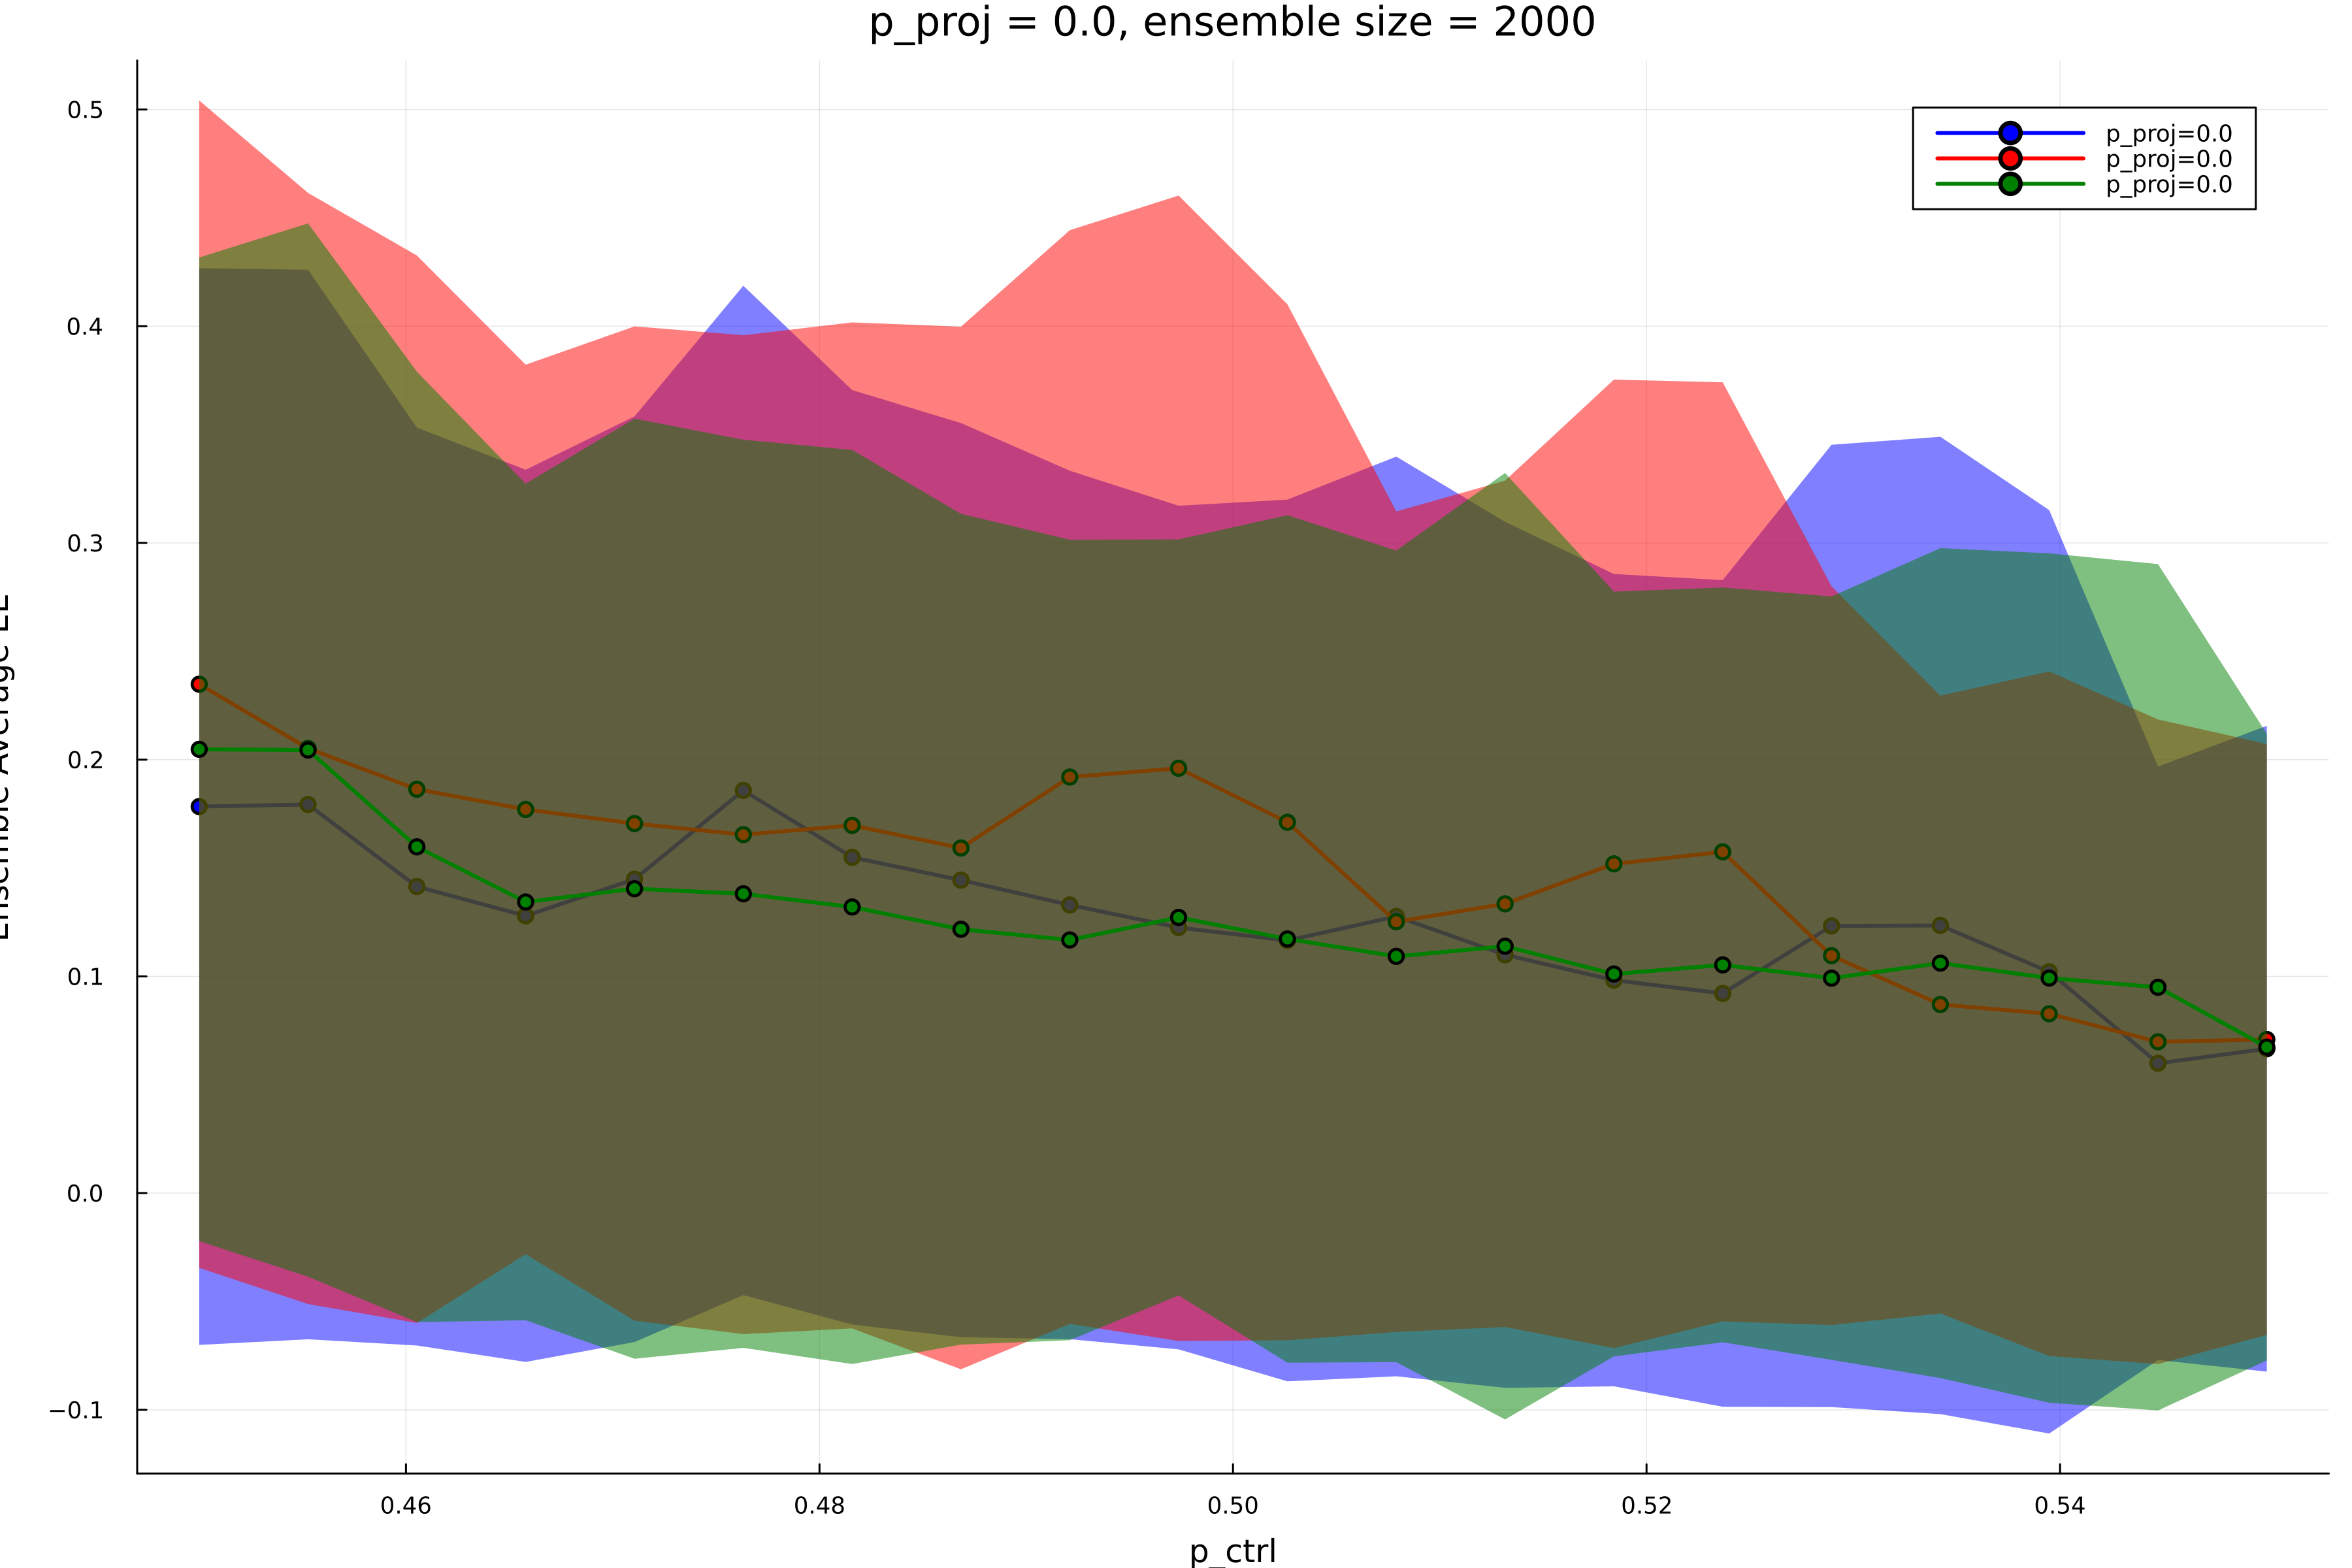
\includegraphics[width=0.8\linewidth]{p_ctrl0.5p_proj0.0.png}
    \caption{Critical scaling analysis at fixed $p_\text{ctrl}=0.5$ and $p_\text{proj}=0.0$, showing data collapse with critical exponent $\nu=4/3$.}
    \label{fig:critical_scaling_pctrl05}
\end{figure}


\section{Issue (May 30, 2025)}

The initial MPS entanglement entropy calculation on small system sizes (L=8,10,12,14) on the cluster came out for the two critical points for testing ($p_\text{ctrl}=0.5$, $p_\text{proj}=0.0$) and ($p_\text{ctrl}=0.4$, $p_\text{proj}=0.75$) with 2000 realizations.

The results are shown in Figure \ref{fig:pctrl0.0pproj0.5(1)} and \ref{fig:pctrl0.4pproj0.7(1)}.

\begin{figure}[H]
    \centering
    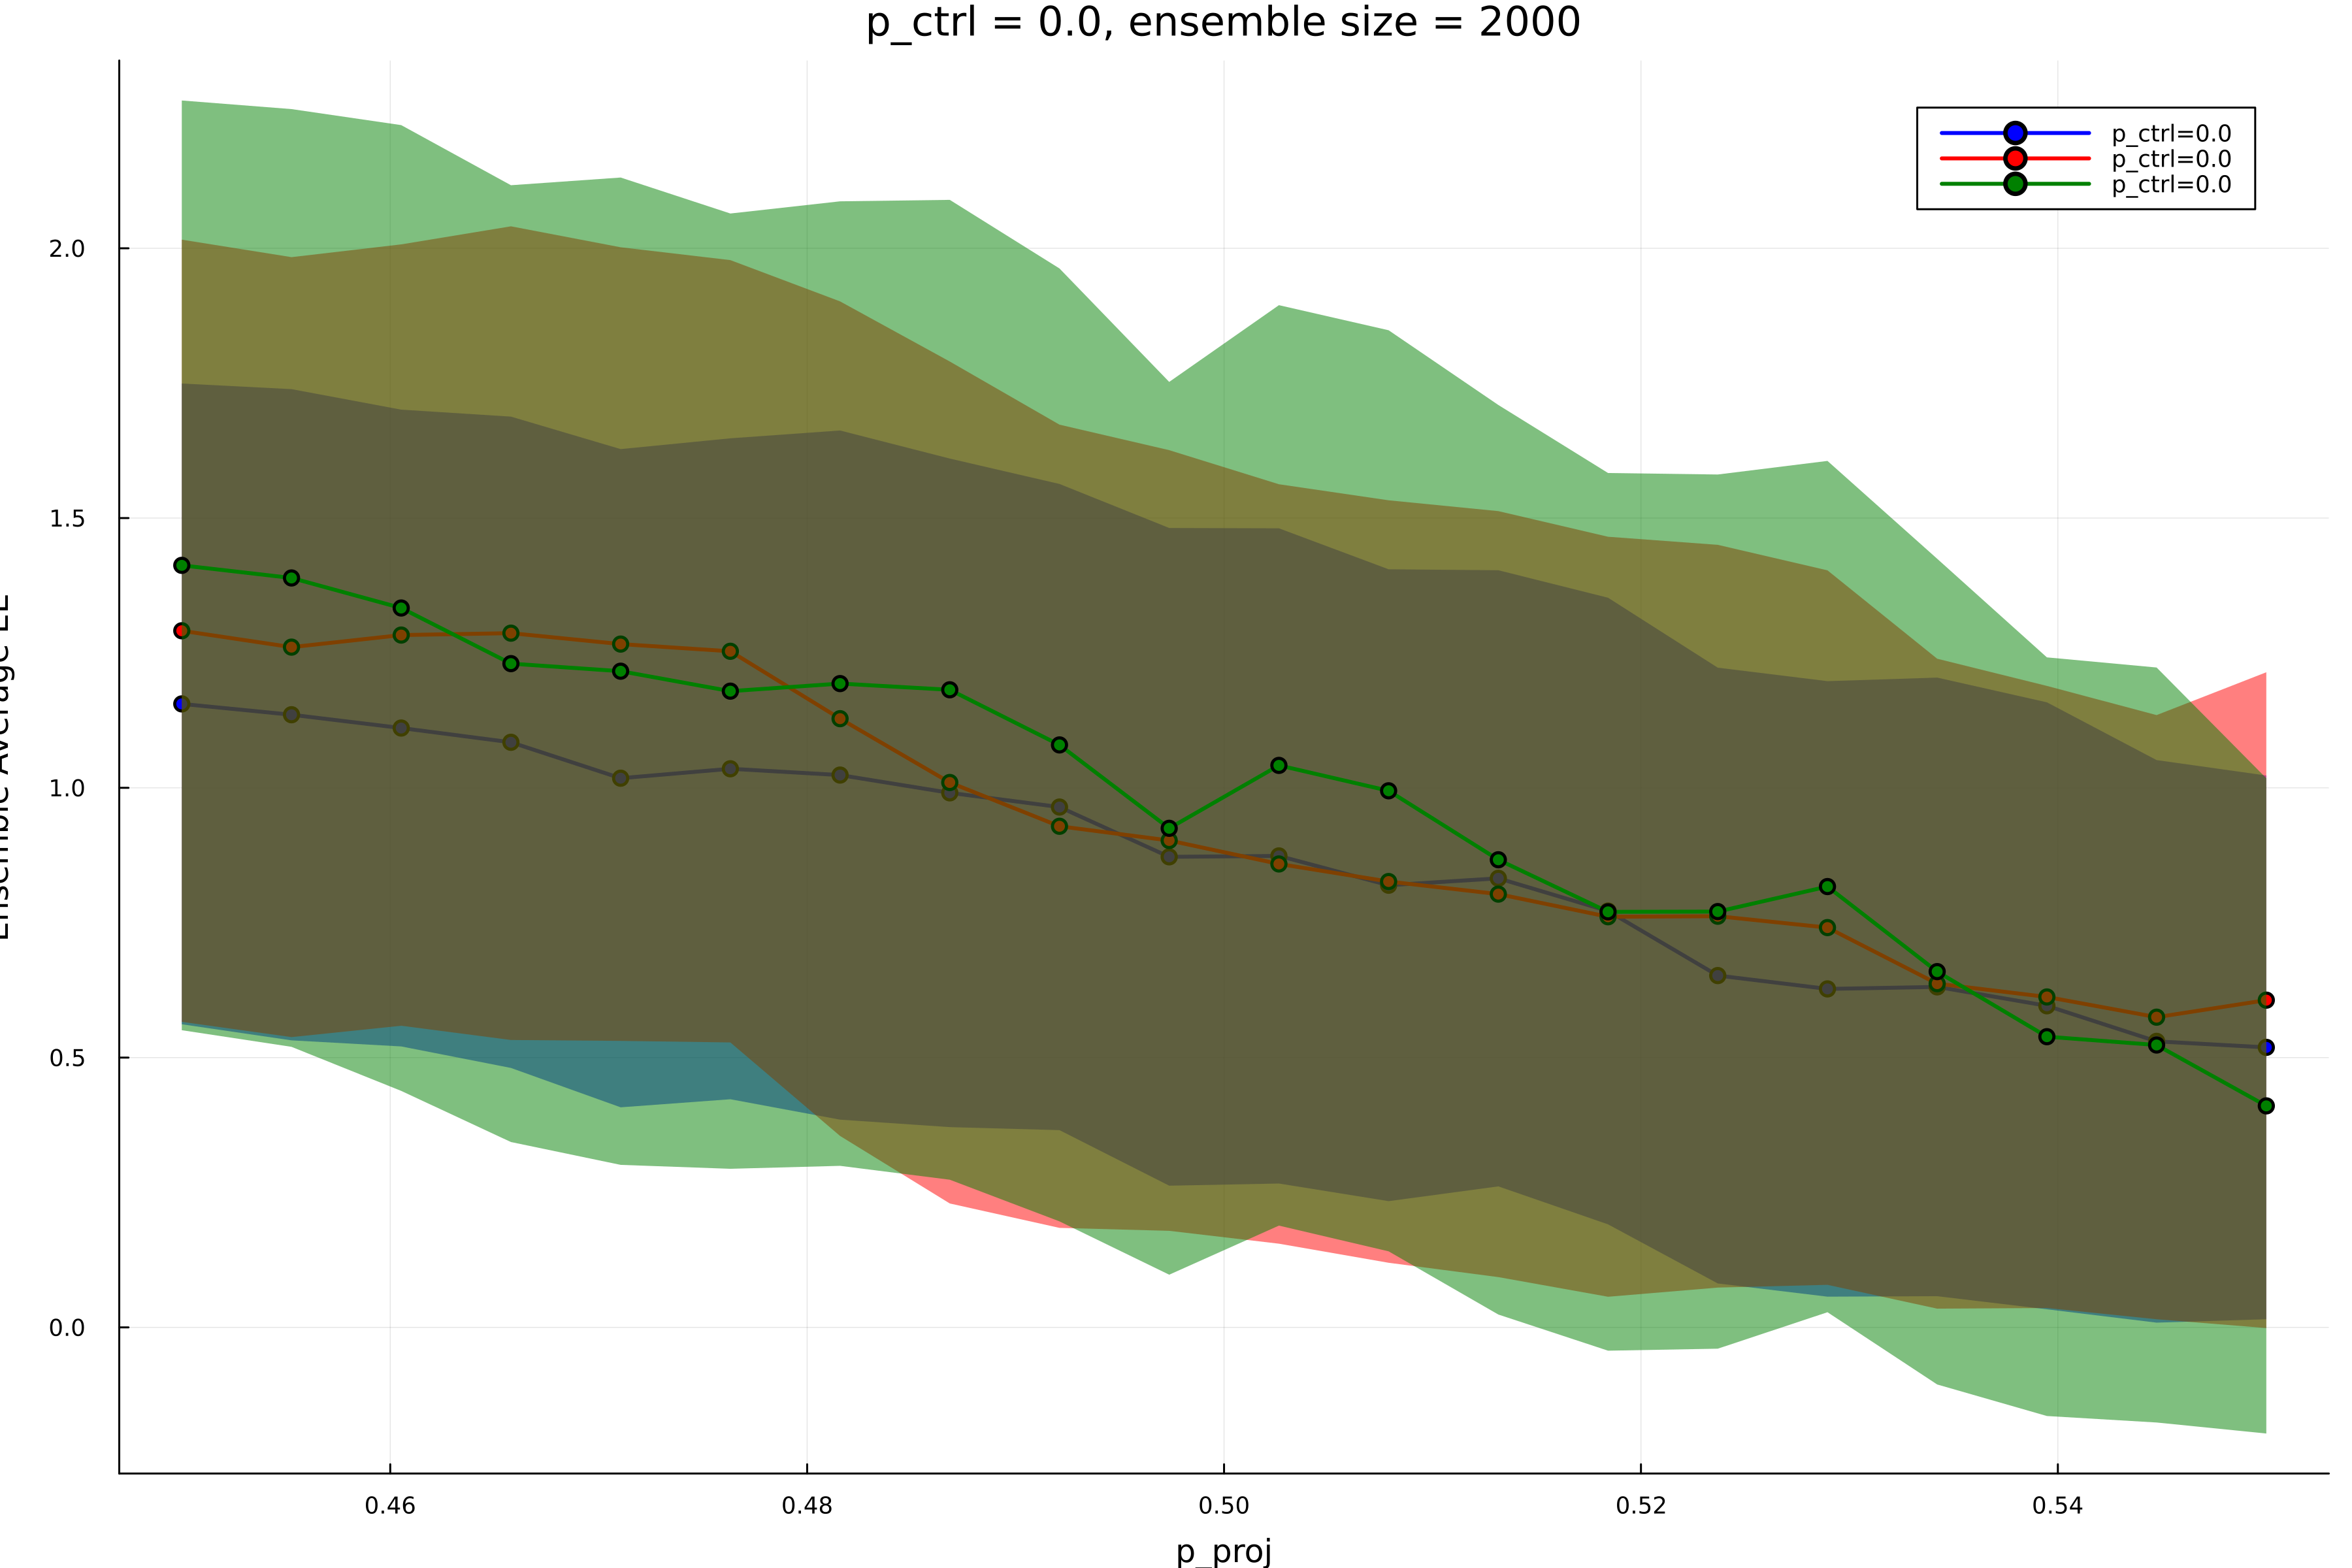
\includegraphics[width=0.8\linewidth]{p_ctrl0.0p_proj0.5(1).png}
    \caption{Entanglement entropy for $p_\text{ctrl}=0.0$ and $p_\text{proj}=0.5$ with L=8,10,12,14.}
    \label{fig:pctrl0.0pproj0.5(1)}
\end{figure}

\begin{figure}[H]
    \centering
    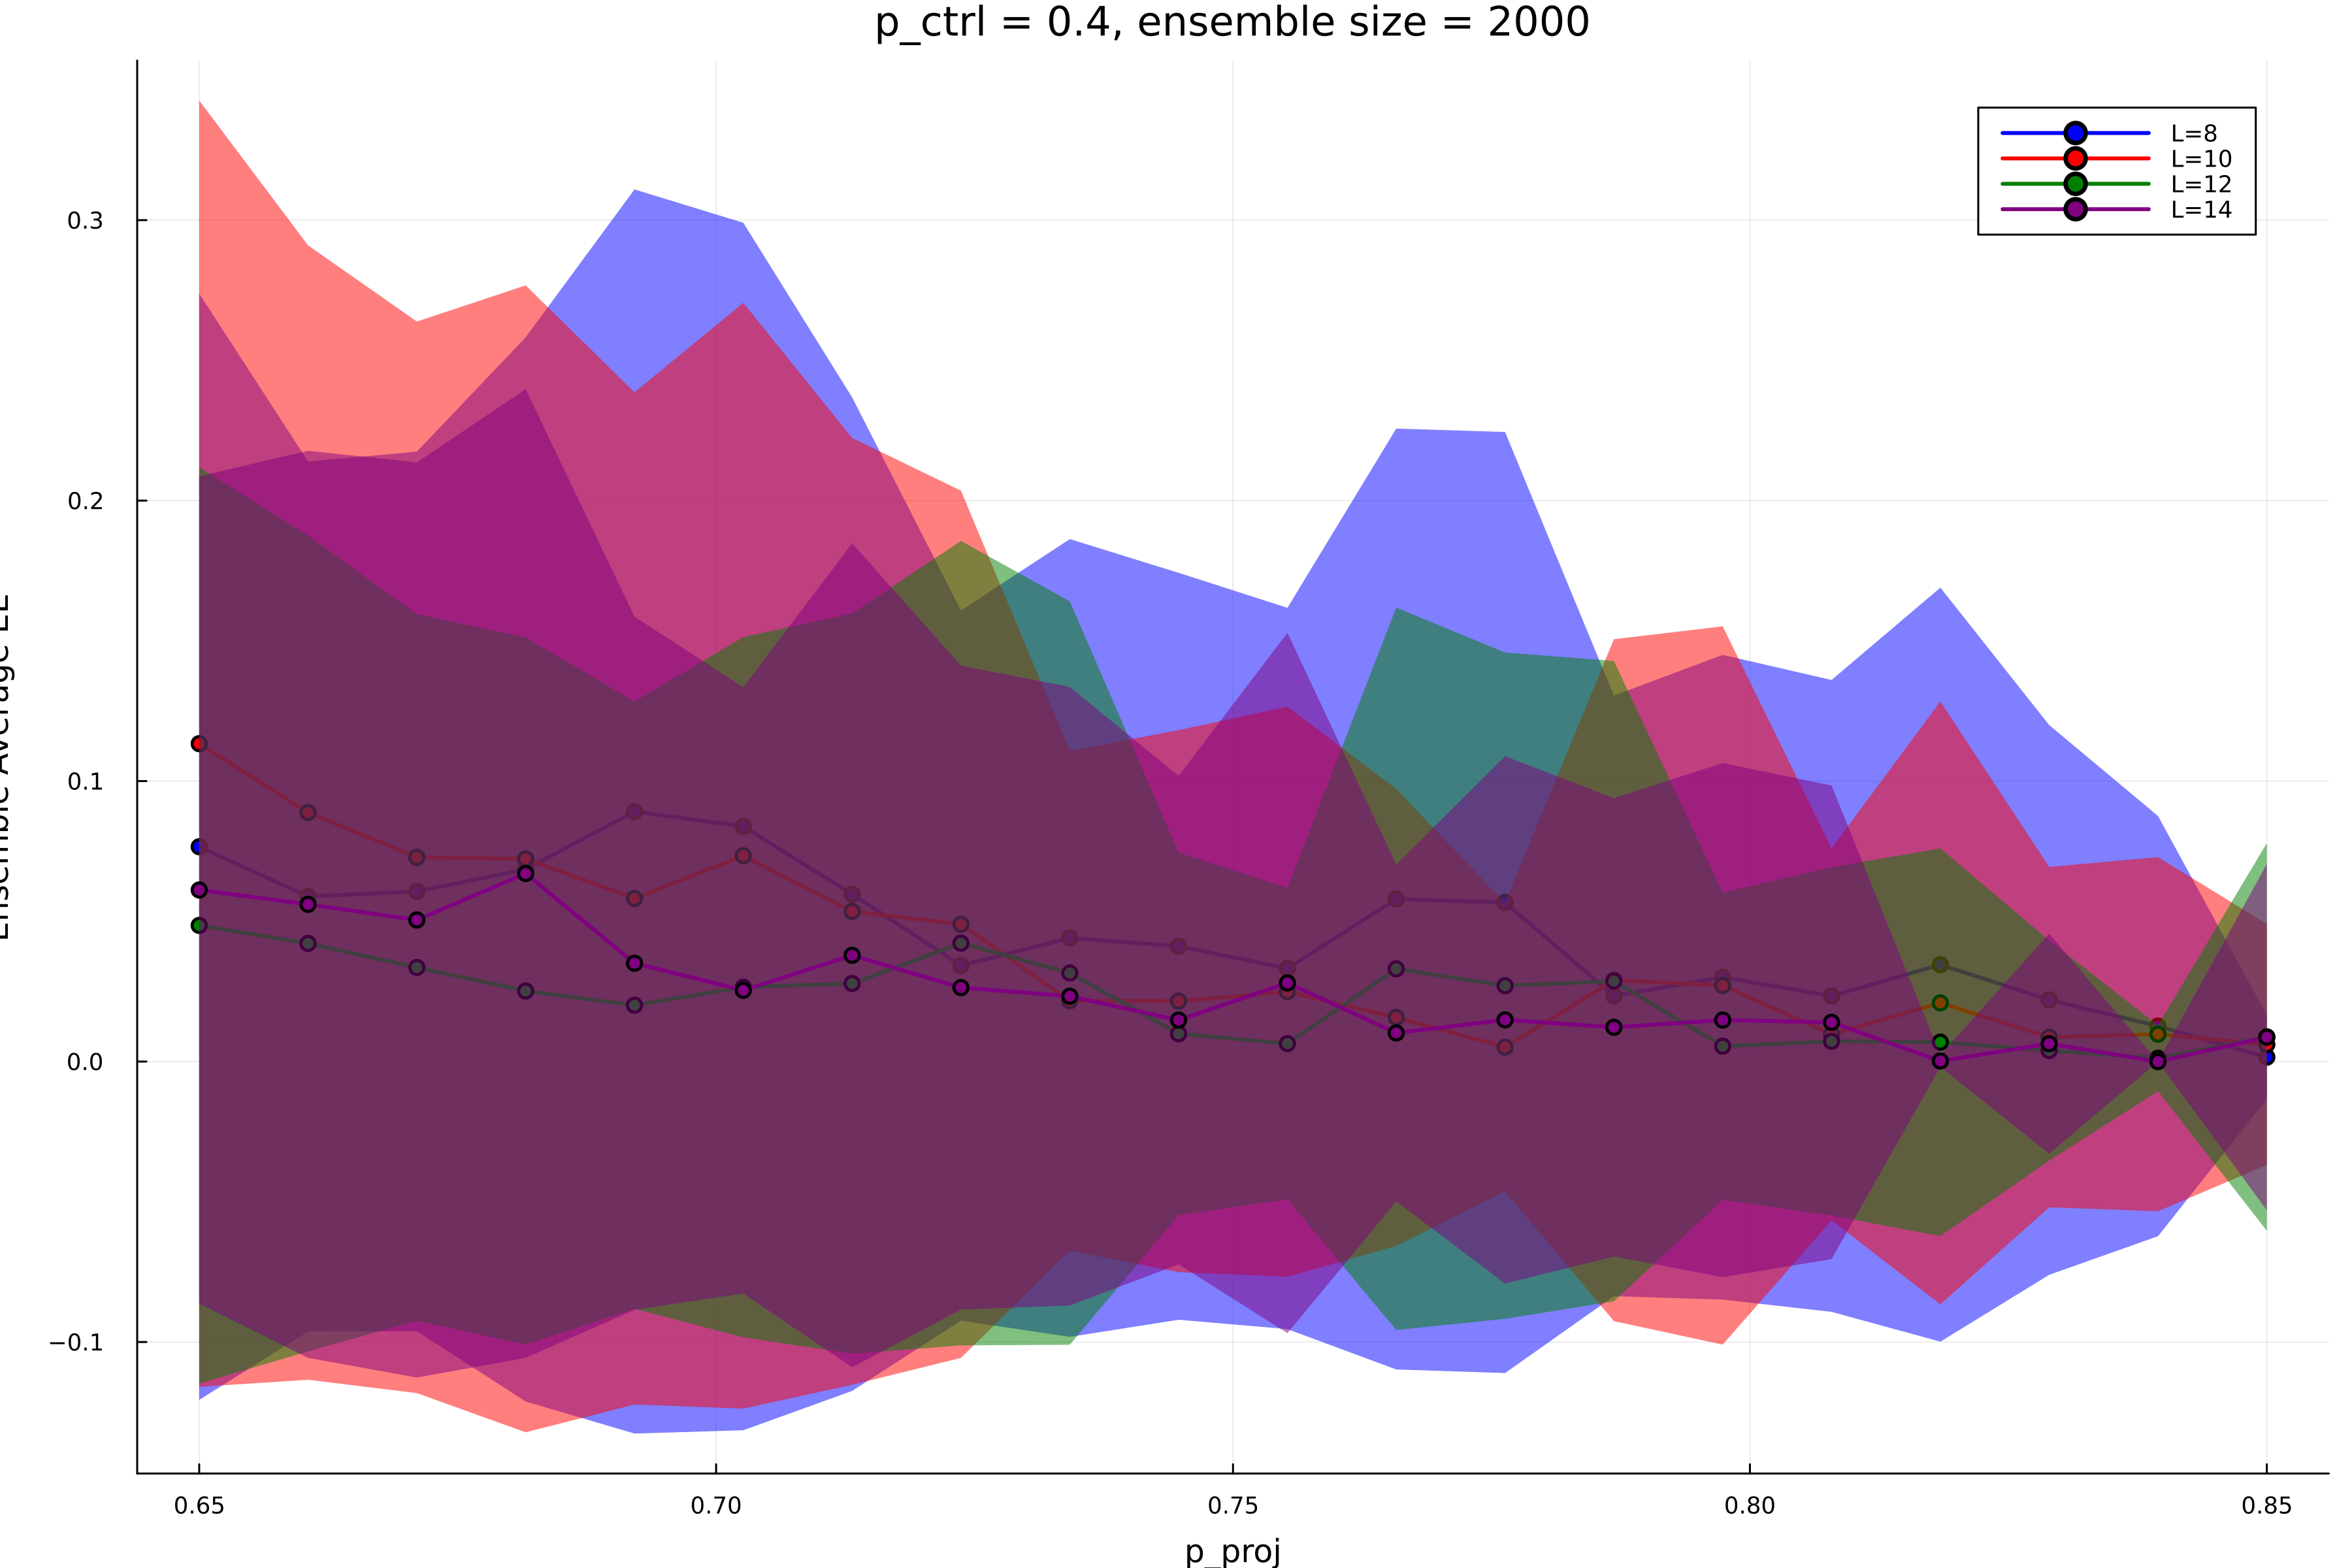
\includegraphics[width=0.8\linewidth]{p_ctrl0.4p_proj0.7(1).png}
    \caption{Entanglement entropy for $p_\text{ctrl}=0.4$ and $p_\text{proj}=0.75$ with L=8,10,12,14.}
    \label{fig:pctrl0.4pproj0.7(1)}
\end{figure}

and as one can see, the entanglement entropy data pretty much completely overlap with each other. This might be normal since we are tkaing a very fine grained scan across the critical points. What I should have done is to do a courser grained scan across the entire range of $p_\text{proj}$ to see whether there is obvious crossing around the expected critical value. Also the finite size effect might also be significant in this initial run.

\par Another minor issue is maybe we should figure out how much memory each run should approximately take. At max, each floating point number takes 8 bytes, for L=14, each statevector has length $2^L = 16384$, so each statevector takes $16384 \times 8 = 131072$ bytes $= 128$ MB. Since we are not storing trajectories, each run should take approximately 128 MB. 

\par On second thought, probably best to push this memory estimation for future: now we can just request a bit more memory per cpu. Going from 4GB to 6GB per cpu worked for L14 calculation. Waiting on the result.

\section{Issue (May 31, 2025)}

The result from previous calculation is in Figure \ref{fig:pctrl0.0pproj0.5coursesmallsize} and \ref{fig:pctrl0.4pproj0.7coursesmallsize}.

\begin{figure}[H]
    \centering
    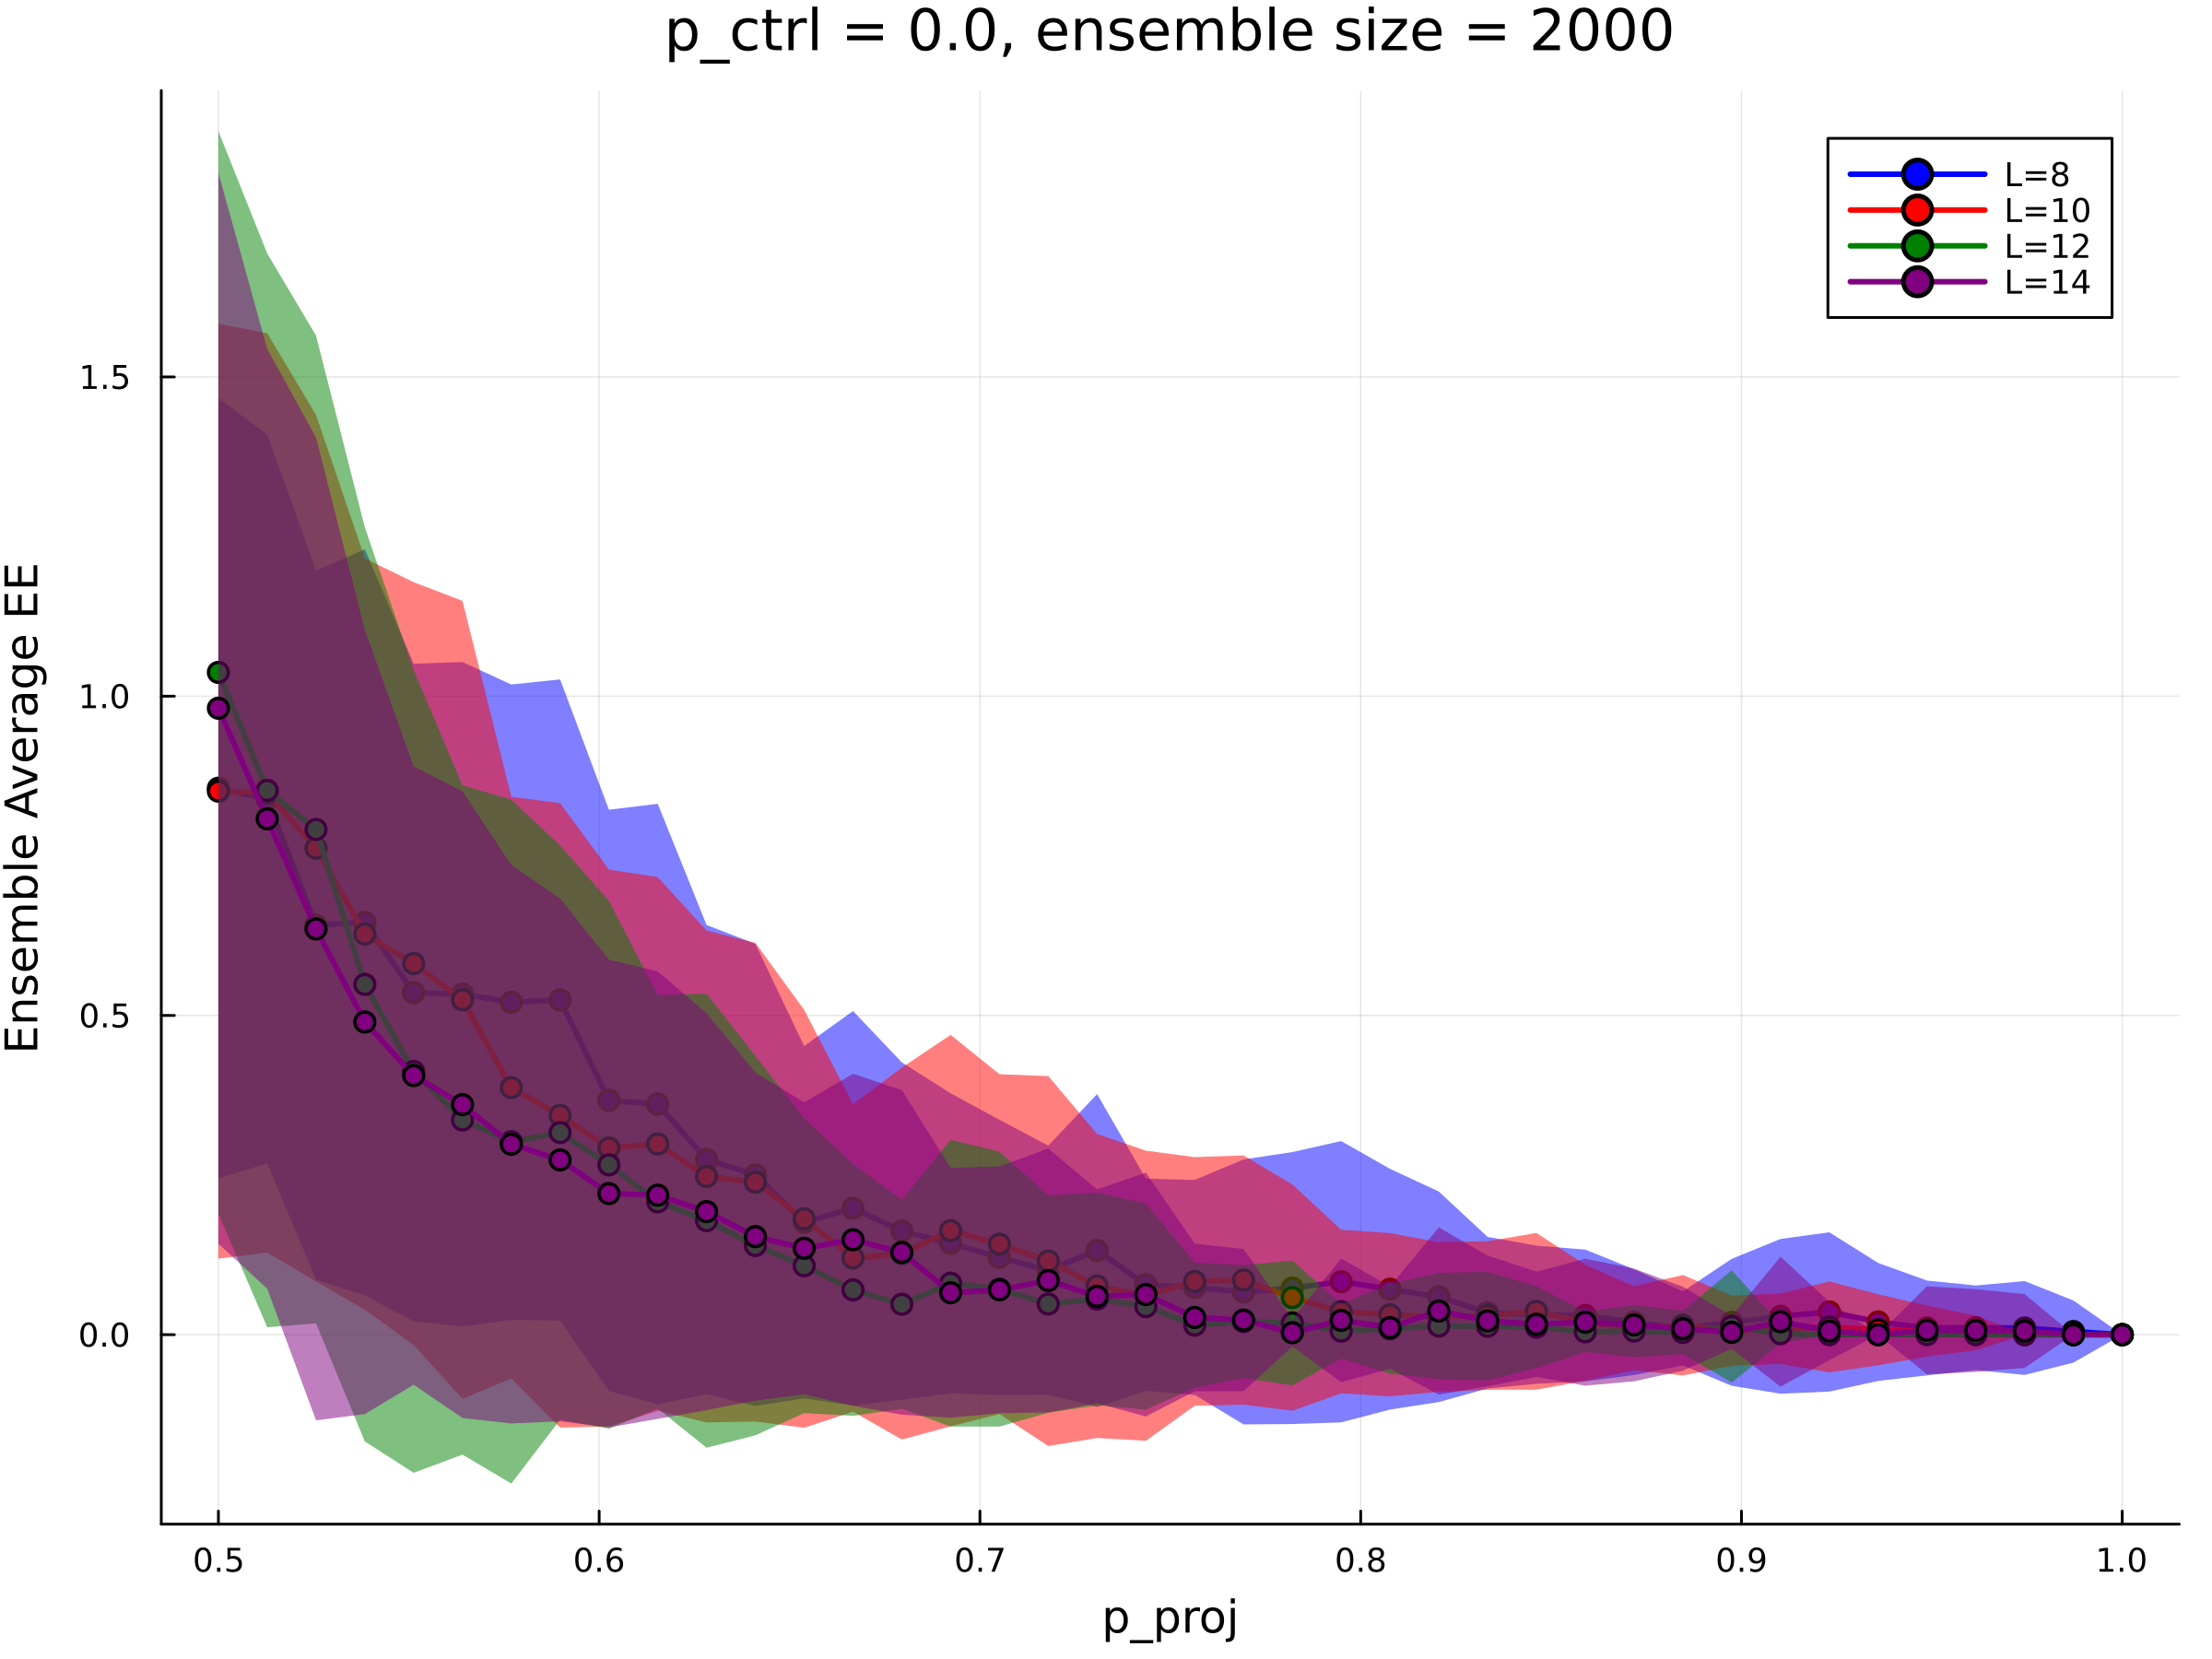
\includegraphics[width=0.8\linewidth]{pctrl0.0pproj0.5coursesmallsize.png}
    \caption{Entanglement entropy for $p_\text{ctrl}=0.0$ and $p_\text{proj}=0.5$ with L=8,10,12,14, with a coarser scan across $p_\text{proj}$.}
    \label{fig:pctrl0.0pproj0.5coursesmallsize}
\end{figure}

\begin{figure}[H]
    \centering
    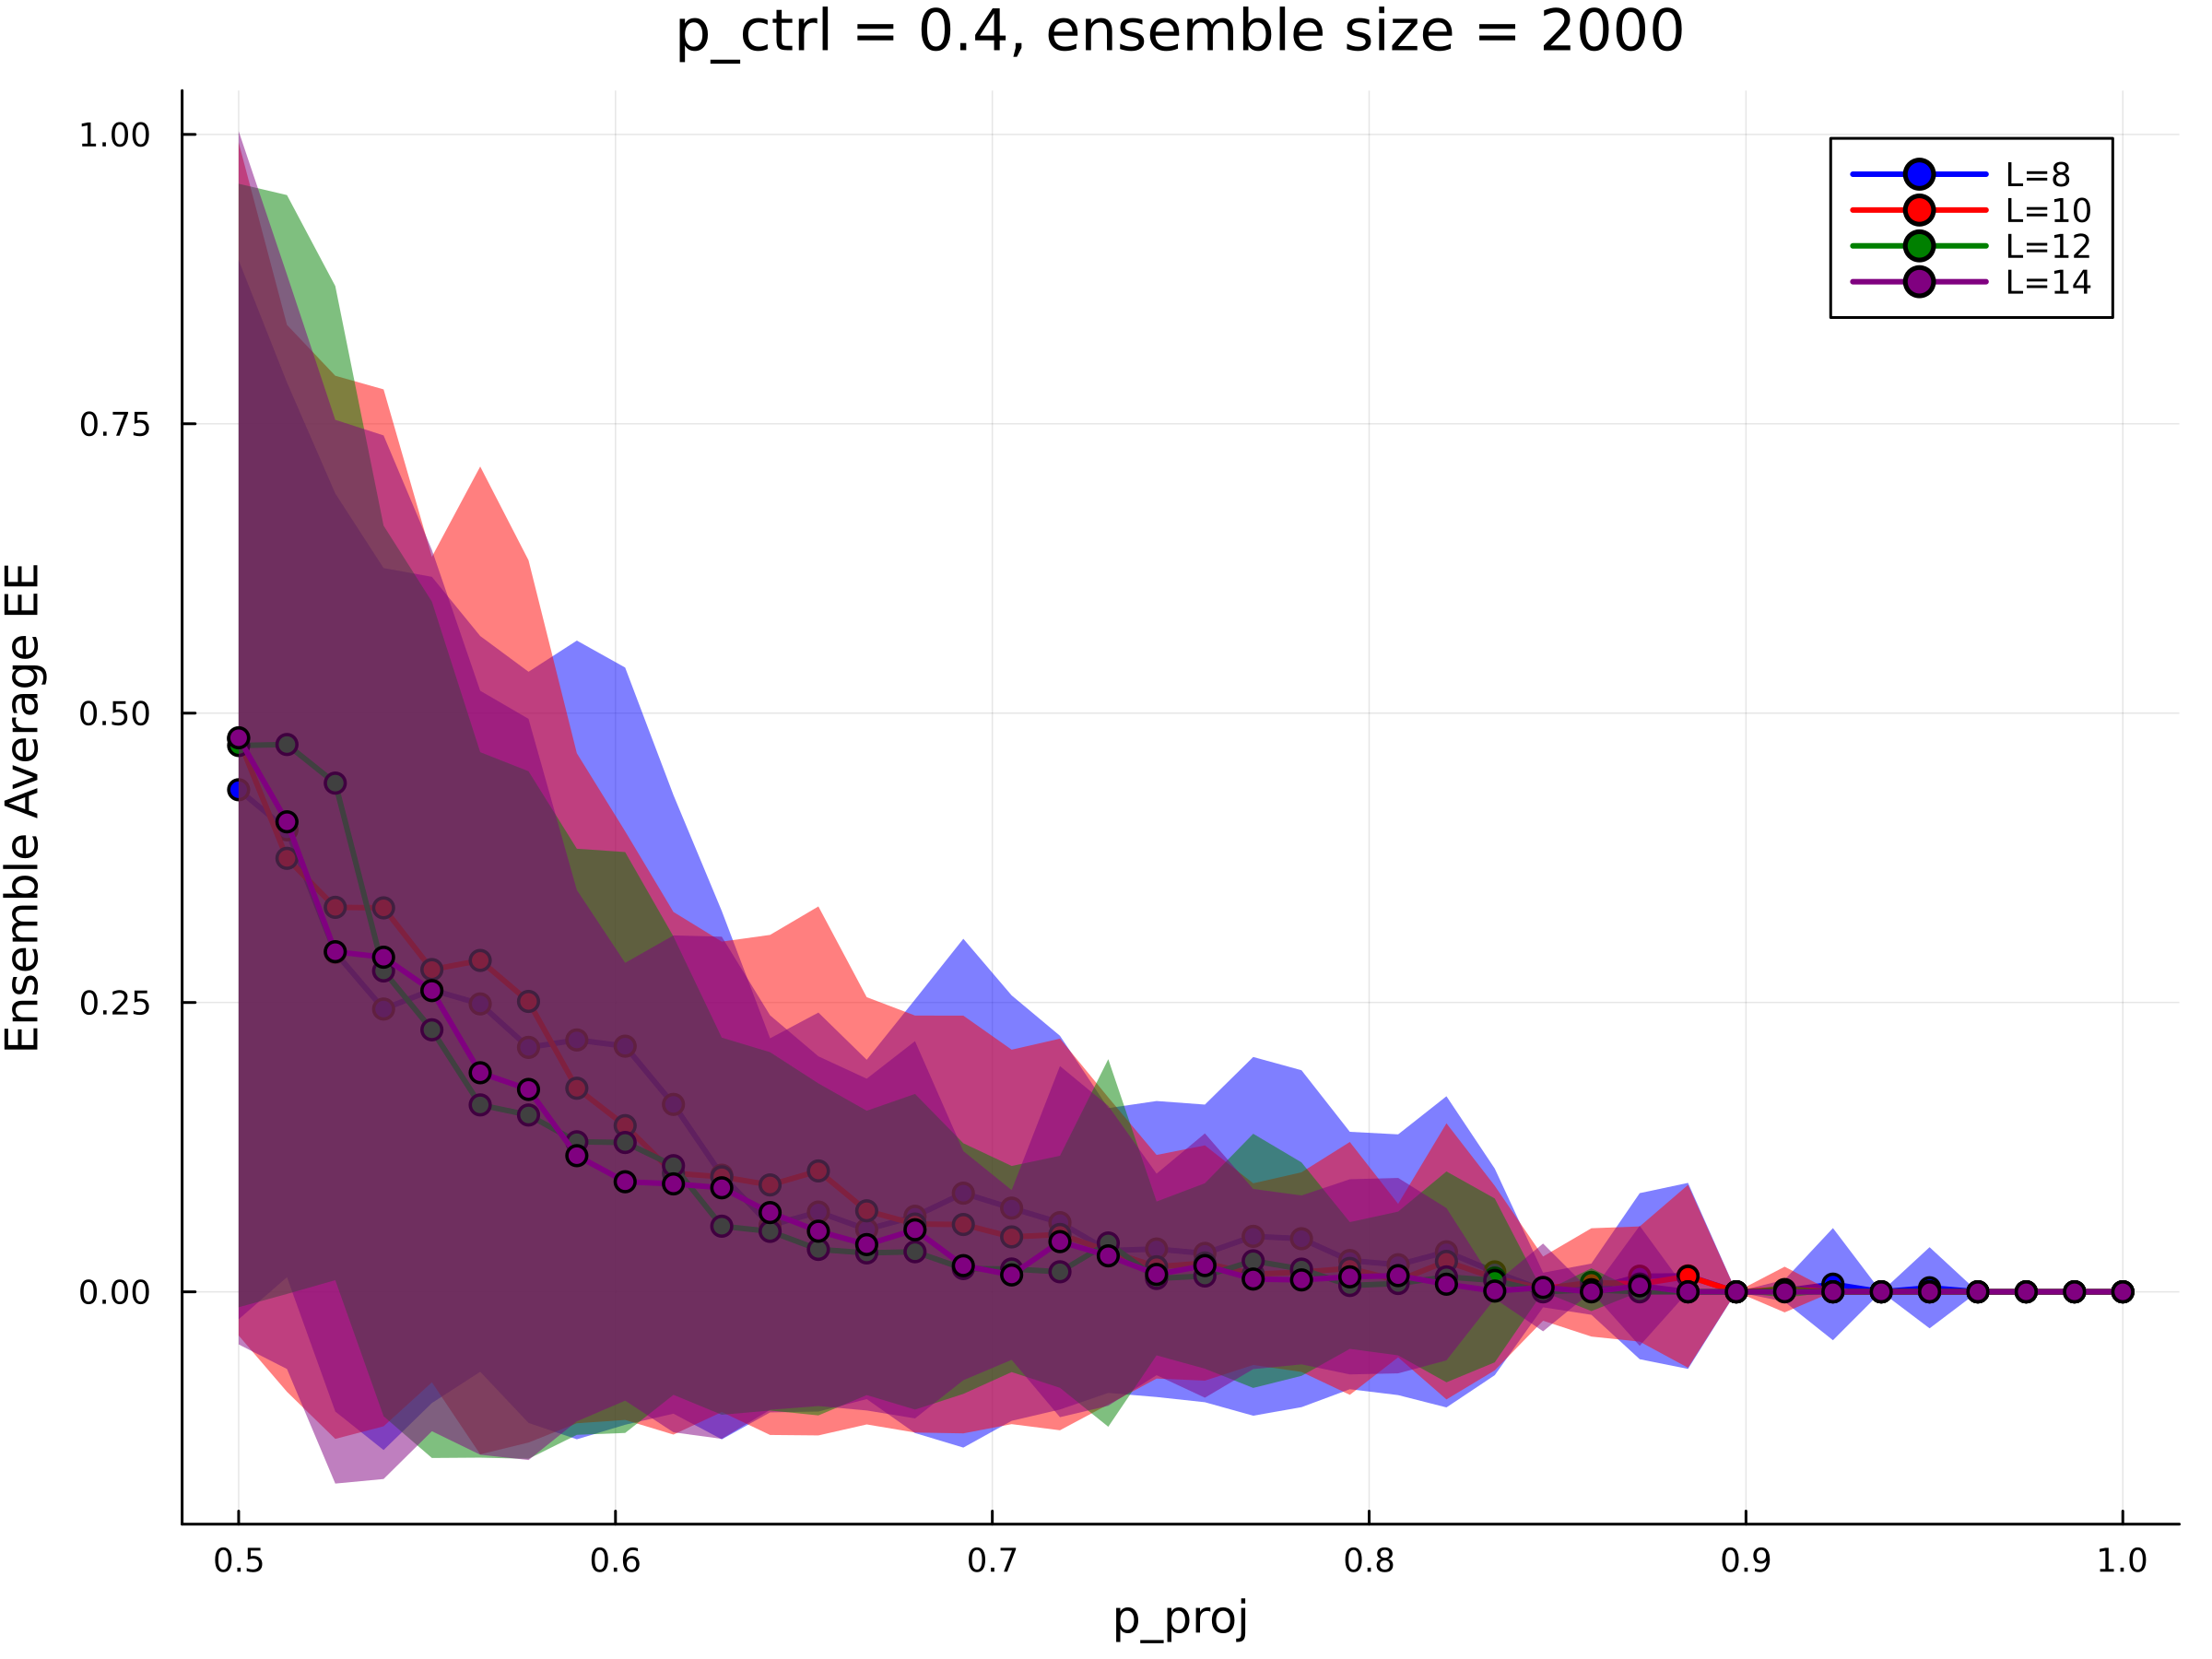
\includegraphics[width=0.8\linewidth]{pctrl0.4pproj0.7coursesmallsize.png}
    \caption{Entanglement entropy for $p_\text{ctrl}=0.4$ and $p_\text{proj}=0.75$ with L=8,10,12,14, with a coarser scan across $p_\text{proj}$.}
    \label{fig:pctrl0.4pproj0.7coursesmallsize}
\end{figure}

As one can see, the ensemble-averaged late-time half-cut entanglement entropy for both critical points overlap almost completely with each other even for a course scan. I don't think a simple finite size effect suffices to explain this. The next step is to first send this result to Haining for his opinion. For me, I think the next step is to try computing ensemble-averaged half-cut entangelment entropy as a function of time and see if I can replicated the published result in Figure 5 of \cite{Pan_2024}. Another worthwhile effort might be to look into how to compute the tripartite mutual information using tensorcrossinterpolation.

\section{Issue (June 3, 2025)}

Upon consulting with Haining, there seems to be several issues with the previous calculation

\begin{itemize}
    \item The crossing of entanglement entropy should only be at $p_\text{ctrl}=0.5$ corresponding to the CIPT. It scales with log L at criticality.
    \item We should use larger L. The small size effect of entanglement entropy is indeed very significant.
    \item The errorbar seems too large: make sure to divide the standard deviation by the square root of the number of realizations to obtain the standard error.
\end{itemize}

Here are the solution efforts:

\begin{itemize}
    \item The crossing of entanglement entropy should only be at $p_\text{ctrl}=0.5$ corresponding to the CIPT. It scales with log L at criticality.

    \textbf{Solution:}

    Submitted new calculations scanning across $p_\text{proj}$ from 0.0 to 1.0 with $p_\text{ctrl}=0.5$. Waiting on the result.

    \item We should use larger L. The small size effect of entanglement entropy is indeed very significant.

    \textbf{Solution:}

    Submitted new calculations with larger system sizes for L = 16, 18, 20. Waiting on the result.

    \item The errorbar seems too large: make sure to divide the standard deviation by the square root of the number of realizations to obtain the standard error.

    \textbf{Solution:}

    Indeed I forgot to divide the standard deviation by the square root of the number of realizations to obtain the standard error. I have fixed this in the codebase.
\end{itemize}

In addition, since oftetimes communication between nodes for a julia job can cause too much computing overhead, and for some of the larger jobs we want to use more CPUs, this means that for computation on larger system sizes we might want to submit multiple jobs for a single system size (for example L=24) and then string them back up together. So we must write a function that takes the number of partitions as input and sends an ensemble size of say 2000 realizations to 5 different nodes each has 20 worker cpus to compute say 400 realizations. Modify \texttt{submit\_multiple\_jobs.sh} for the computation and storage of partitioned data and add a post-data-processing .jl script which averages the partition data.

Finished implementing the partitioned data computation, but I suspect something is not correct. The test for L=16 is way too slow. Since we are using 5 nodes and 20 cpu's per node, the computation for each node should be 400 realizations which should take only around one hour but the total job is now taking more than 5 hours. 


\section{Issue (June 6, 2025)}

Computation with the current codebase has several issues, and below each of them I note their respective solutions.

\begin{itemize}
    \item The most immediate issue is the memory usage. For L=16, the memory per cpu usage is 12GB. If we try to request 20 CPUs on a single node, the total memory usage is 240GB, making it very low priority for slurm to schedule this. For larger system sizes, we will not even a node equipped with so much memory.

    \textbf{Solution:}

    Although we cannot request something like 20 CPUs per node, we can request as many jobs as we want. So for L=16 for example, 20 p values and 2000 realizations, we can request 200 jobs and each job consisting of computing 20 p values over 20 realizations. We limit one worker cpu per job but does not limit which node the job is scheduled on. This takes the maximal advantage of the ``embarassing parallelization'' of the cluster. 

    \item Another important question is what bond dimension we should choose.

    \textbf{Solution:}
    
    This deserves a systematic investigation for whatever p fixed value we choose. I think there are two ways of doing this: 

    \begin{itemize}
        \item We can compute the ensemble-averaged late-time half-cut entanglement entropy for different bond dimensions vs p scan value for a fixed p fixed value. The behavior of the curve should approach a limit as the bond dimension goes to its maximal value $2^{L/2}$. 
        \item We can also for a fixed point on the phase diagram (fixing both $p_\text{ctrl}$ and $p_\text{proj}$ values), compute the time-evolution of the ensemble-averaged half-cut entanglement entropy for different bond dimensions. This should also approach a plateau as the bond dimension goes to its maximal value $2^{L/2}$.
    \end{itemize}

    The first method is Haining's method, so let's try that first.

    \par In addition, I also need to figure out how much memory per cpu different size computations need. 
\end{itemize}

\section{Issue (June 9, 2025)}

Fixed and improved the memory benchmarking code to provide more reliable measurements. The updated code now:
\begin{itemize}
    \item Reliably extracts maximum memory consumption
    \item Calculates average time per realization
    \item Automatically generates a summary.txt file in each experiment's data folder
\end{itemize}

\section{Issue (June 10, 2025)}

Investigation focused on memory requirements for specific parameter regions:
\begin{itemize}
    \item Discovered significant variation in memory usage depending on p-fixed values
    \item When p\_proj is fixed to 0.5, scanning through p\_ctrl from 0.45 to 0.55 requires 8G per CPU for maxdim 100 and L18
    \item This unexpected memory usage pattern suggests parameter-dependent computational complexity
\end{itemize}

\section{Issue (June 11, 2025)}

Developed a systematic workflow for memory and time estimation:

\textbf{Workflow Steps:}
\begin{enumerate}
    \item Request interactive session on compute node (1 CPU, 40G memory, 1 hour)
    \item Execute sequence:
    \begin{itemize}
        \item Load singularity module
        \item Run Julia with system image and optimization flags
        \item Monitor process memory usage with timestamps
        \item Extract max/min memory requirements from logs
    \end{itemize}
\end{enumerate}

\textbf{Implementation Details:}
\begin{itemize}
    \item Identified issue with memory measurement units in 'top' output
    \item Fixed memory calculation to properly handle unit conversions
    \item Implemented automatic logging of memory statistics to summary.txt
\end{itemize}

\section{Technical Journal Entries}

\subsection{June 11, 2023}
\begin{itemize}
    \item \textbf{Objective:} Developed workflow for memory and runtime testing
    \item \textbf{Workflow Implementation:}
    \begin{enumerate}
        \item Request interactive session: 1 CPU, 40GB memory, 1 hour
        \item Load singularity module
        \item Execute Julia script with specific parameters:
            \begin{itemize}
                \item Using sysimage for optimization
                \item Parameters: scan\_type=p\_ctrl, p\_fixed=0.5, L=18
                \item Maximum bond dimension: 500
            \end{itemize}
        \item Implemented memory logging system
        \item Fixed memory benchmark code to correctly measure memory consumption
        \item Added functionality to generate summary.txt with max memory and avg time metrics
    \end{enumerate}
\end{itemize}

\subsection{June 12, 2023}
\begin{itemize}
    \item \textbf{Key Observations:}
    \begin{itemize}
        \item Proposed using ensemble-averaged late-time half-cut entanglement entropy for bond dimension selection
        \item Identified need to verify p\_proj=0.5 as appropriate boundary
        \item Noted memory usage concerns: observed 3GB usage for single initial random MPS
        \item Hypothesized excessive package precompilation causing memory overhead
    \end{itemize}
\end{itemize}

\subsection{June 13, 2023}
\begin{itemize}
    \item \textbf{Performance Analysis:}
    \begin{itemize}
        \item Tested new sysimage performance
        \item Investigated non-terminating Julia processes
        \item Memory allocation analysis:
            \begin{itemize}
                \item L8: 1.5GB allocation, 81\% compilation time
                \item L16: 14GB allocation, 40\% compilation time
            \end{itemize}
        \item Memory scaling with T\_max:
            \begin{itemize}
                \item T\_max = 1: 655,792 maxresident
                \item T\_max = 2: 811,144 maxresident
                \item T\_max = 3: 931,348 maxresident
                \item T\_max = 4: 962,452 maxresident
                \item T\_max = 2L^2: 2,444,668 maxresident \(L=16\)
            \end{itemize}
    \end{itemize}
\end{itemize}

\subsection{June 23-24, 2023}
\begin{itemize}
    \item \textbf{Performance Evaluation:}
    \begin{itemize}
        \item Initial success with run\_CT\_MPS\_1-3.jl script
        \item Discovered performance parity with run\_CT\_MPS\_ensemble.jl
        \item Identified potential source of memory discrepancy:
            \begin{itemize}
                \item Different ITensor versions (v0.6 vs newer version)
                \item Additional package compilation overhead
            \end{itemize}
    \end{itemize}
\end{itemize}

\subsection{July 1, 2023}
\begin{itemize}
    \item \textbf{Progress Report:}
    \begin{itemize}
        \item Successfully replicated Haining's codebase
        \item Implemented parallelization: result seems promising (see Figure \ref{fig:average_EE_vs_p_ctrl})
        \item Achieved computation for L=18 and L=20 with improved memory efficiency
        \item Created new GitHub repository: CT\_MPS\_mini
        \item Key finding: ITensor version impact on memory usage
            \begin{itemize}
                \item Old version (0.6): More compact
                \item New version: Extended functionality but higher memory overhead
            \end{itemize}
    \end{itemize}
    \item \textbf{Next Steps:}
    \begin{itemize}
        \item Conduct bond dimension study
        \item Analyze memory usage patterns
    \end{itemize}
\end{itemize}

\begin{figure}[H]
    \centering
    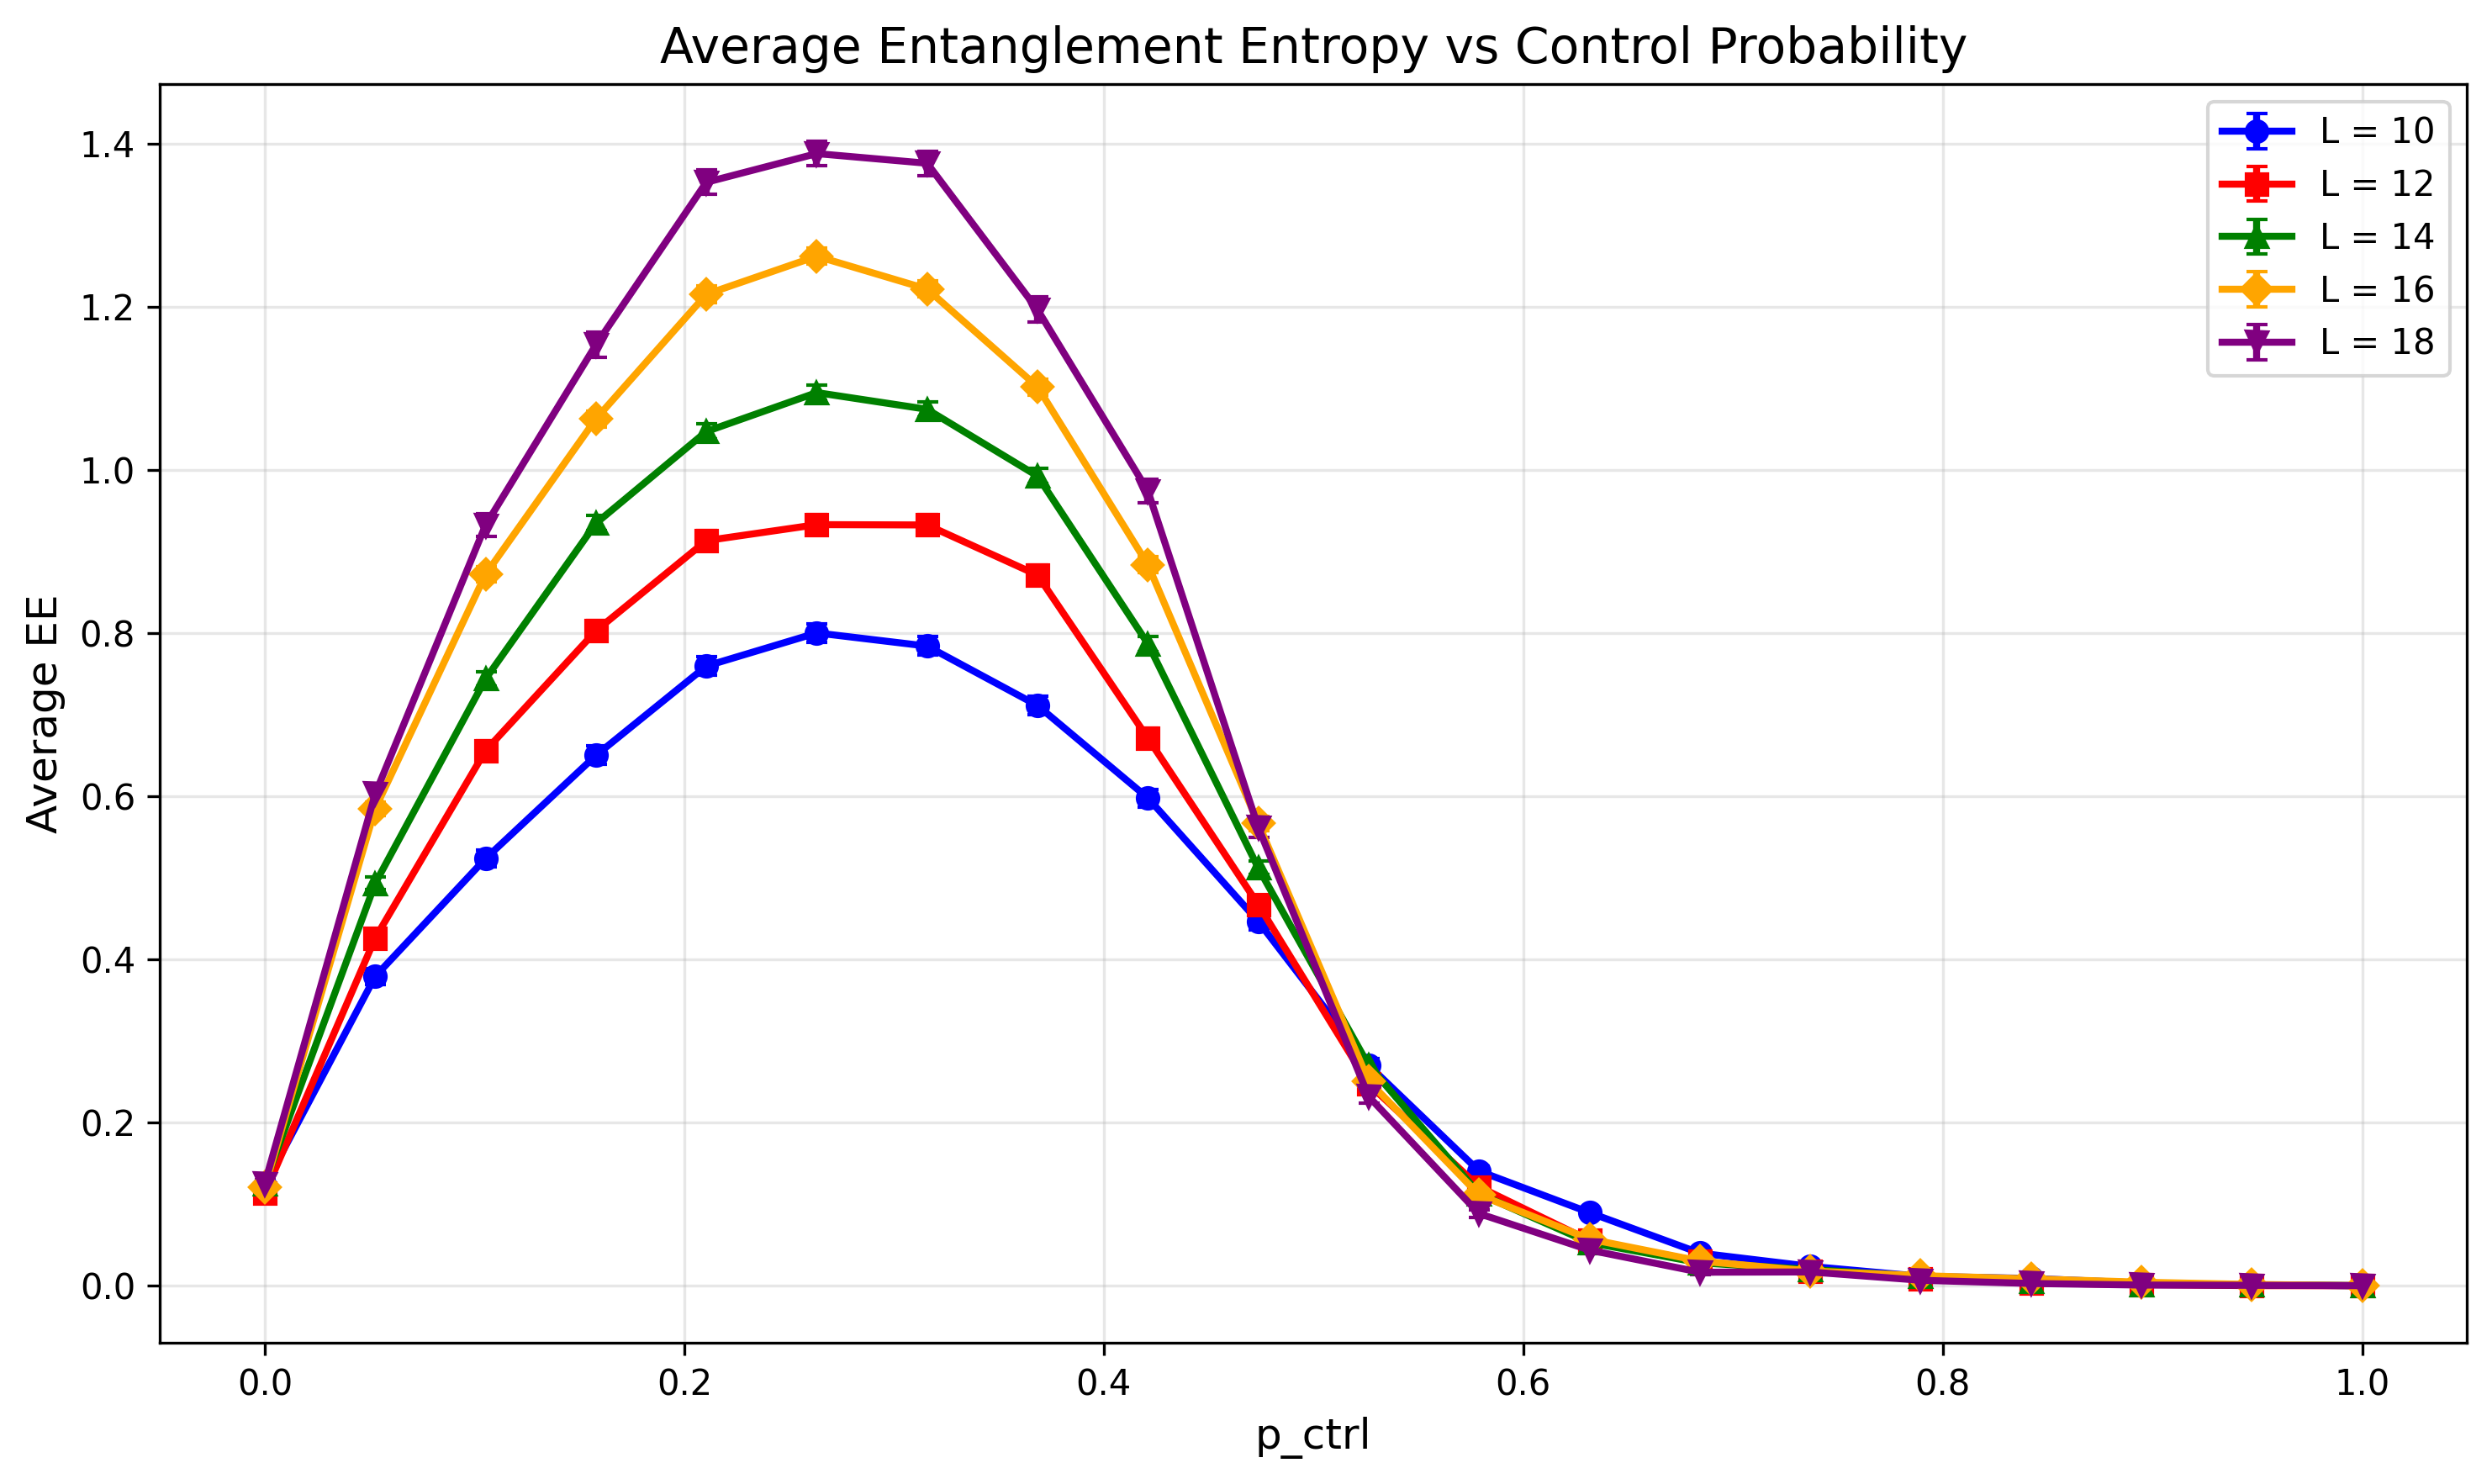
\includegraphics[width=0.8\linewidth]{average_EE_vs_p_ctrl.png}
    \caption{Average EE vs p\_ctrl for L=18 and L=20.}
    \label{fig:average_EE_vs_p_ctrl}
\end{figure}

\bibliographystyle{plainnat}
\bibliography{references}

\end{document} 